\documentclass[parskip, twoside, accentcolor=tud9b, colorback, breaklinks, noresetcounter, noheadingspace, pdfencoding=unicode, 11pt, bigchapter, numbersubsubsec, numbers=noenddot, linedtoc, longdoc]{tudreport}

%%% ============ Package Section ============


%% main packages
\usepackage[utf8]{inputenc}  			% file encoding: UTF-8
\usepackage[ngerman]{babel}			    % language selection
\usepackage{microtype} 					% typographic refinements

%% tables
\usepackage{booktabs}					% alternative table style
\usepackage{multirow}					% support tabular cells spanning multiple rows
\usepackage{longtable}					% multi-page tables
\usepackage{tabularx}					% tables with adjustable cell width

%% figures / placement
\usepackage{multicol}					% support for multi-column sections
\usepackage{subfig}
% \usepackage{subcaption}					% support multiple figures within one figure
\usepackage{float}						% support forced "here" placement
\usepackage{wrapfig}					% support figures with text wrapped around

%% graphics
\usepackage{graphicx}					% enhanced graphics support
\usepackage{xcolor}		% color support (already loaded by "pgf")
\usepackage{soul}
%\usepackage{pgf}						% graphics creation environment backend

\usepackage{tikz}						% graphics creation environment frontend
\usepackage{tikz-cd}
\usepackage{import}
\usepackage{multicol}
% 
\usepackage{pgfplots}					% graph plotting for pgf/tikz
\pgfplotsset{compat=1.12, grid style={gray,dotted}}

\usetikzlibrary{external} %% comment out to stop externalization of tikz pictures
\tikzexternalize[optimize=false, prefix=tikz-external/] % path to store the externalized stuff in
%\tikzset{external/system call={lualatex \tikzexternalcheckshellescape -halt-on-error-interaction=batchmode -jobname "\image" "\texsource"}, force remake = false}
% \tikzset{external/force remake = false}
\tikzexternalize

%% mathematics
\usepackage{amsmath}					% enhanced mathematics support
\usepackage{nicefrac}					% nice inline fractions
\usepackage{icomma}						% support comma as decimal separator

%% source code
%\usepackage{listings}					% support for source code listings
\usepackage[many]{tcolorbox}
\tcbuselibrary{listings}

%% misc
\usepackage{paralist}					% enhanced list styles and environments
\usepackage{textcomp} 					% additional symbols
\usepackage[nottoc, numbib]{tocbibind}	% ToC modification: do not include ToC, number bibliography heading
\usepackage{enumerate}					% simplified enumeration formatting (counter style)
\usepackage{enumitem}					% enhanced enumeration manipulation
\usepackage[stable]{footmisc}			% support footnotes in section titles
% \usepackage{makeidx}					% support for makeindex
\usepackage{xstring}					% support for string manipulation
\usepackage{xkeyval}					% extended key-value decoder
%\usepackage{soul}						% enhanced highlighing support
\usepackage[super]{nth}					% superscript 1st, 2nd ...
\usepackage[english=american]{csquotes}	% automatic quotation marks
\usepackage{datetime}					% date and time formatting
\usepackage{etoolbox}					% LaTeX programming toolbox
\usepackage{xpatch}						% enhanced latex patching support
\usepackage{xspace}						% support for content-dependent spacing
\usepackage[binary-units=true,exponent-product=\cdot]{siunitx}	% support values with SI units and binary units
\usepackage{ifdraft}					% allow commands that depend on the draft/final option
\usepackage{framed}						% environmant drawing a frame around the text
\usepackage{comment}					% selectively include / exclude text
\usepackage{verbatim}					% use reimplemented verbatim environment
\usepackage{outlines}					% support for simplified lists
\usepackage{rotating}					% support for rotated floating environments
%\usepackage{circuitikz}					% add circuit symbols for tikz/pgf
\usepackage[percent]{overpic}			% suppoerr image overlays
\usepackage{pict2e}						% allow graphical vector with floating point units
\usepackage[section]{placeins}					% provide \FloatBarrier command
\usepackage[normalem]{ulem}				% support for underlining in text mode (withough breaking \em)
\usepackage[version=4]{mhchem}			% support for chemistry stuff
\usepackage{chngcntr}					% commands for influencing counters
\usepackage{varwidth}					% variable width minipages
\usepackage[referable,flushleft]{threeparttablex}	% table with footnotes, reqired for own hypertabular environment
\usepackage{afterpage}					% support for delayed commands (invoked on next page)
\usepackage{calc}						% latex arithmetics
%\usepackage{tikz-timing}				% timing diagrams for tikz/pgf
\usepackage{xparse}						% enhanced commands interface
%\usepackage{todonotes}
\usepackage[disable]{todonotes}					% support for todo notes
% \usepackage[list=true, listformat=simple]{subcaption}					% subfigure support
\usepackage{cellspace}					% enhanced spacing in tables
\usepackage{blindtext}
%\usepackage{rotfloat}
%\usepackage{lscape}
\usepackage{titlesec}					% title format manipulation

%% referencing (do not change package order!)
\usepackage{varioref}					% improved referencing
\usepackage[american, breaklinks]{hyperref} 	% cross-referencing and PDF metadata (direct loading in non-PDF/A mode only)
\usepackage{hyperxmp}
\usepackage[sort,compress,noabbrev,nameinlink]{cleveref}	% simplified referencing
\usepackage[numbers]{natbib}
\bibliographystyle{unsrt}

%% hacks
\usepackage{scrhack}					% fixes some latex interoperability issues

%% others
% \usepackage{array}
% \newcolumntype{M}[1]{>{\centering\let\newline\\\arraybackslash\hspace{0pt}}p{#1}}

%%% ============ Configuration and Refinements ============

%% Load special configuration (flags)

%% ============== Configuration flags ============== 

\def\outputstyledraft{} 		% enables draft style if active

\DeclareFontFamily{OT1}{pzc}{}
\DeclareFontShape{OT1}{pzc}{m}{it}{<-> s * [0.900] pzcmi7t}{}
\DeclareMathAlphabet{\mathpzc}{OT1}{pzc}{m}{it}

%% ============== Hacks ============== 

%% apply \textbf to math mode as well (via \boldmath)
\let\oldtextbf=\textbf
\renewcommand\textbf[1]{{\boldmath\oldtextbf{#1}}}


\renewcommand{\textrightarrow}{\ensuremath{\rightarrow}\xspace}

\renewcommand\plparsep{1ex}									% vertical list item spacing

%% calculate longtable width
\newlength{\longtablewidth}
\setlength{\longtablewidth}{0.7\linewidth}
\addtolength{\longtablewidth}{-\marginparsep}
\addtolength{\longtablewidth}{-\marginparwidth}

%% marginalia (side node) configuration
\newif\ifTUDmargin\TUDmarginfalse
	% \TUDmargintrue 					% uncommenting the line below will enable marginalia
	\ifTUDmargin\makeatletter
	\TUD@setmarginpar{2}
\makeatother\fi

%% automatic quotation mark adjustment settings
\MakeInnerQuote{|}						% define character for inner quotation marks (to be replaced by correct quotation marks by csquotes)
\MakeOuterQuote{"}						% define character for outer quotation marks (to be replaced by correct quotation marks by csquotes)

%% configuration of enumerations
%\setlist{noitemsep}					% disable whitespace in enumerations

%% xspace exceptions
\xspaceaddexceptions{"}					% remove whitespace in front of quotation marks if \xspace command is used

%% change format for subfigures (style 'simple'): Add small space in between
\makeatletter
\g@addto@macro\p@subfigure{\,}
\makeatother

%\pgfplotsset{compat=newest}

\addparagraphcolumntypes{X}				% Register tabularx column type for use with celltypes package

%\titleclass{\chapter}{straight}			%% start new chapter on same page by default

%% listings style for plain text reports
\lstdefinestyle{report}{
	language={},
	captionpos=b,
	frame=single,
	keepspaces=true,
	breakatwhitespace=false,
	breaklines=true,
	captionpos=t,
	literate={\-}{}{0\discretionary{-}{}{-}},
	basicstyle=\tiny
}


%%% ============ Color Definitions ============

\definecolor{optionalcolor}{named}{lightgray}				% define color to be used for optional parts
\definecolor{shadecolor}{named}{optionalcolor}		% define color to be used for optional parts using the "optionalbox" environment


%%% ============  Other Hacks ============

%%% ------------  URL Hacks ------------

\urlstyle{rm}													% use \rmfamily instead of default \ttfamily style for URL links


%%% ============ Commands and Environments ============

%% Chapter without pagebreak
\makeatletter
\newcommand\Chapter{\par\vspace{2cm}
                    \global\@topnum\z@
                    \@afterindentfalse
                    \secdef\@chapter\@schapter}

%% Bring book-type's frontmatter/mainmatter/backmatter commands to tudreport
\newcommand\frontmatter{\cleardoublepage\pagenumbering{roman}}
\newcommand\mainmatter{\cleardoublepage\pagenumbering{arabic}}
\newcommand\backmatter{\if@openright\cleardoublepage\else\clearpage\fi}



\makeatother

%%% ============ Document Information ============

%% Thesis date definitions
\newdate{reportdate}{\the\day}{\the\month}{\the\year}
\newdate{topicdate}{13}{11}{2017}

%% Thesis information
\newcommand{\reportauthor}{Rainer Stellnberger, \\Julian Buschbaum, Benjamin Lars Northe}
%\newcommand{\reportgroup}{1}
%\newcommand{\reportsubsubtitle}{Subsubtitle}
\newcommand{\reporttitle}{Seminarausarbeitung Projektseminar Beschleunigertechnik}
\newcommand{\reporttopic}{Parameteranalyse Impedanz Rinkern-Kurzschluss}
\newcommand{\reportkeywords}{-}



\hypersetup{%
	pdftitle={\reporttitle},
	pdfauthor={\reportauthor},
	pdfsubject={\reporttitle},
	pdfkeywords={\reportkeywords},
	pdfview=FitH,
	pdfstartview=FitV,
	pdfcopyright={\copyright 2018 by \reportauthor.  All rights reserved.},
	pdfinfo={
				Copyright={\copyright Date by \reportauthor.  All rights reserved.}
			},
	}



%%% ============ Title Page Setup ============

%%% Title page configuration
%\title{\fontsize{31}{31}\selectfont\reporttitle} % unmodified font-size (32,32?) would introduce an ugly line break
%\subtitle{\reporttopic\vspace{0.5em}}
%\subsubtitle{Autor: \reportauthor\\Datum: \displaydate{reportdate}}
%\setinstitutionlogo{../Material/logo/ies_logo_vectorized}

%% Title page from IES Template
\title{\reporttopic}
\subtitle{\reporttitle\ von \reportauthor}
\subsubtitle{%
    Betreuer: Jens Harzheim\\
    Start: 15.04.2018 \textbar\ Ende: 27.09.2018\\
    Fachgebiet Beschleunigertechnik\hfill\textbar\hfill Prof.\,Dr.-Ing.\, Harald Klingbeil}
%\uppertitleback{(\textaccent{\textbackslash uppertitleback})}
%\lowertitleback{(\textaccent{\textbackslash lowertitleback})\hfill\today}
\institution{}
\setinstitutionlogo{../Inputfiles/Graphics/Logo/temf.png}

%%% ============ Custom Commands ============

%% Remove whitespace in front of this commands
\newcommand{\erasewhitespacebefore}{\leavevmode\unskip}

%% Comment to print arrow (workaround for the missing \textrightarrow in TUD design fonts)
\newcommand{\arrowright}{$\rightarrow$\xspace}

%% Add \tocless in front of \section to omit adding section to ToC, without affecting numbering
\newcommand{\nocontentsline}[3]{}
\newcommand{\tocless}[2]{\bgroup\let\addcontentsline=\nocontentsline#1{#2}\egroup}

%% Rotate content 90° on odd and 270° on even pages
\newcommand{\sidewaysbox}[1]{\ifthispageodd{\rotatebox{90}{#1}}{\rotatebox{270}{#1}}}

%% Captions that include references at the end that should not be shown in the list of figures / tables
%% #1:	The caption, without references
%% #2:	The references
\newcommand{\capref}[2]{\caption[#1]{#1 #2}}

%% Print something rotated by 90 degrees
%% #1:	The part to print rotated
\newcommand\tabrotate[1]{\rotatebox{90}{{~#1}}}

\newcommand{\bitstyle}[1]{#1}
\newcommand{\bytestyle}[1]{\textbf{#1}}

%% Format for assembler operations
\newcommand{\op}[1]{\texttt{\MakeUppercase{#1}}}

%%% ============ Document ============

\begin{document}

%% Title Page %%%%%%%%%%%%%%%%%%%%%%%%%%%%%%%%%%%%%%%%%%%%%%%%%%%%%%%%%%%%%%%%%%
\frontmatter
\hypersetup{pageanchor=false}
\maketitle
\hypersetup{pageanchor=true}
\cleardoublepage

%% Erklärung
%%%%%%%%%%%%%%%%%%%%%%%%%%%%%%%%%%%%%%%%%%%%%%%%%%%%%%%%%%%%%%%
%\pagestyle{empty}
%\pagenumbering{roman} .
%\chapter*{Erklärung}

Ich versichere hiermit, die vorliegende Arbeit selbstständig und ohne
fremde Hilfe angefertigt zu haben. Die verwendete Literatur und
sonstige Hilfsmittel sind vollständig angegeben.\\
Ich versichere, dass die Abgaben der digitalen und gedruckten Fassung identisch sind. \vspace{8ex}

%\noindent
\begin{tabularx}{\textwidth}{@{}lp{.3cm}p{3cm}p{.3cm}X@{}}
  \multicolumn{4}{@{}r}{Darmstadt, 13.~November~2017} & \dotfill \\[-.7ex]
                  &&    && \small\ Unterschrift
\end{tabularx}

%\vspace{\fill}
\vspace*{4cm}

%\section*{Erklärung}

%\noindent 
%Mit der Veröffentlichung der Diplomarbeit durch das Fachgebiet
%Rechnersysteme erklären wir uns einverstanden: \vspace{8ex}
%
%%\noindent
%\begin{tabularx}{\textwidth}{@{}lp{3cm}X@{}}
%  Diplomarbeiter & \dotfill & \dotfill \\[-.7ex]
%                  & \small\ Datum    & \small\ Unterschrift \\[8ex]
%  Betreuender Professor & \dotfill & \dotfill \\[-.7ex]
%                  & \small\ Datum    & \small\ Unterschrift \\[8ex]
%  Betreuender Assistent & \dotfill & \dotfill \\[-.7ex]
%                  & \small\ Datum    & \small\ Unterschrift \\[10ex]
%                  &            & \ Fachgebietsstempel
%\end{tabularx}
%
%\cleardoublepage

%\end{document}

%%% Local Variables: 
%%% mode: latex
%%% TeX-master: t
%%% End: 


%% Table of Contents %%%%%%%%%%%%%%%%%%%%%%%%%%%%%%%%%%%%%%%%%%%%%%%%%%%%%%%%%%%
\cleardoublepage
\pagestyle{plain}
\pdfbookmark{\contentsname}{contents}
\tableofcontents
\cleardoublepage

%% Tabellen und Abbildungen %%%%%%%%%%%%%%%%%%%%%%%%%%%%%%%%%%%%%%%%%%%%%%%%
% List of figures:
\listoffigures
\cleardoublepage
% % List of tables:
% \listoftables
% \cleardoublepage

%% Abk\"urzungsverzeichnis und Symbolverzeichnis %%%%%%%%%%%%%%%%%%%%%%%%%%%%
\chapter*{Abk\"urzungsverzeichnis}
\begin{tabular}{p{0.2\textwidth} p{0.7\textwidth}}
\textbf{Abk\"urzung} & \textbf{Beschreibung} \\
 & \\
MA & magnetic alloy \\
RK & Ringkern \\
<<<<<<< HEAD
GSI & GSI Helmholtzzentrum f\"ur Schwerionenforschung GmbH\\
=======
GSI & Gesellschaft f\"ur Schwerionenforschung \\
NA & Network Analyzer\\
>>>>>>> 699c838b2c1928b020b3f7dfead72a908fac4304
KS & Kurzschluss \\
BNC & Bayonet Neill Concelman: F\"ur Oszilloskope verwendeter Koaxialstecker \\
CST & Computer Simulation Technology \\
PE & Polyethylen \\
RLC & Netzwerk aus Widerstand, Induktivit\"at und Kapazit\"at \\
ESB & Ersatzschaltbild\\
\end{tabular}

\cleardoublepage

\chapter*{Symbolverzeichnis}

\begin{tabular}{p{0.2\textwidth} p{0.7\textwidth}}
\textbf{Symbol} & \textbf{Beschreibung und Einheit}\\
 & \\
$\omega$ & Kreisfrequenz \\

$Z_{rk}$ & Impedanz des MA-Ringkerns \\
$L_{rk}$ & Induktivit\"at des MA-Ringkerns \\
$R_{rk}$ & Wirkwiderstand des MA-Ringkerns \\
$\underline{\mu}_r$ & Komplexe, dissipative Permeabilit\"atskonstante\\
% $\mu^{\prime}$ & \\
% $\mu^{\prime\prime}$ & \\
$N$ & Anzahl der Ringkerne\\
$d$ & Ringkerndicke\\
$r_i$ & Innendurchmesser eines Ringkerns \\
$r_o$ & Au\ss{}endurchmesser eines Ringkerns \\
$\underline{\varepsilon}_r$ & Komplexe, dissipative Dielektrizit\"atskonstante\\
$\underline{Z}_{ges}$ & Gemessene Impedanz an der Testbox \\
$R_{box}$ & Wirkwiderstand des RLC-Modells der Testbox \\
$L_{box}$ & Induktivit\"at des RLC-Modells der Testbox \\
$C_{box}$ & Kapazit\"at des RLC-Modells der Testbox \\
$a_{max}$ & Maximale relative Abweichung eines Messparameters \\
$a_{percent}$ & Maximale relative Abweichung eines Messparameters(Prozent) \\


\end{tabular}





%% Main Part %%%%%%%%%%%%%%%%%%%%%%%%%%%%%%%%%%%%%%%%%%%%%%%%%%%%%%%%%%%%%%%
%\mainmatter
\pagestyle{headings}
\pagenumbering{arabic}

\chapter{Einleitung}\label{chap:einleitung}
	\section{Theorie}

Bei der Gesellschaft für Schwerionenforschung(GSI) werden in der Gruppe Ring-RF Systems unter anderem  Barrier Bucket Systeme entwickelt, welche zur Modifikation der longitudinalen Strahldynamik, wie etwa zum Zusammenf\"uhren oder Verdichten eines oder mehrerer Strahl-Bunches verwendet werden k\"onnen. 
Das Grundprizip der Barrier Bucket Systeme besteht darin, Teilchen zwischen zwei Potentialbarrieren zu begrenzen. Diese Potentialbarrieren k\"onnen verschiedene Formen aufweisen, h\"aufig werden einzelne Sinus-Pulse verwendet~\citep{harzheim2016modeling}~\citep{lee1997particle}. Durch \"Anderung der Barrieren, wie etwa der Variation des Abstandes zwischen einzelnen Barrieren, k\"onnen somit die Teilchen verdichtet oder verteilt werden.
Die Barrier Bucket Systeme Systeme verwenden unter anderem magnetische Ringkerne als Last. Vorteil ist, dass mit diesem Aufbau ein Tuning der Resonanzfrequenz m\"oglich ist (siehe Kapitel 4 in \citep{Klingbeil2015} bzw. Kapitel 2 in \citep{bast2017ba}).
\par
Die MA(magnetic alloy)-Ringkerne weisen dabei eine charakteristische Impedanz auf, welche nicht einer idealen Spule entspricht, sondern vielmehr ein dissipatives Verhalten zeigt. Eine genauere Herleitung kann in \citep{Klingbeil2015} gefunden werden und liefert folgenden Zusammenhang. 


\begin{align}
Z_{rk} = R_{rk} + j\omega L_{rk}\label{eq_01}\\
L_{rk} = \frac{Nd\mu^\prime}{2\pi}\cdot ln(\frac{r_o}{r_i})\label{eq_02}\\
R_{rk} = \omega L_{rk} \frac{\mu^{\prime\prime}}{\mu^{\prime}}\label{eq_03}
\end{align}




	\section{Aufgabenstellung}
%     \begin{enumerate}
%         \item Untersuchung verschiedener Parameter von Kurzschlüssen um Ringkerne und deren Einfluss auf die Impedanz
%     \end{enumerate}
Die Impedanz der Ringkerne wirkt sich auf den Teilchenstrahl im Beschleuniger aus. Diese Auswirkung soll möglichst reduziert werden, wenn keine Beschleunigung vorliegen soll.
\par
Die Aufgabe des Projektseminars besteht deshalb darin, zu analysieren, in wie weit das Kurzschlie\ss{}en der MA-Ringkerne innerhalb der Kavit\"at die Impedanz dieser verringern kann. Dazu sind mehrere Parameter der Kurzschl\"usse, sowie deren Anzahl zu untersuchen.
\par
\textcolor{blue}{
Damit die Ergebnisse auch mit anderen Parametern untersucht werden k\"onnen, wird der gesamte Aufbau samt der Halterung f\"ur den Ringkern, sowie der Kurzschl\"usse, ausgehend von dem bereits bestehenden Modell aus der Bachelorarbeit von Denys Bast~\citep{bast2017ba}, in CST modelliert.}
\par
\textcolor{blue}{
Abschlie\ss{}end werden sowohl die Simulationsergebnisse, als auch die Messergebnisse unter \"Anderung der Paramter gegen\"ubergestellt. Dadurch kann eine pr\"aferierte Anordnung zum Kurzschlie\ss{}en der MA-Ringkerne bestimmt werden. Diese Schritte werden in den folgenden Kapiteln erl\"autert.}
\par 
\textcolor{red}{Alternativ:}

 
	
\chapter{Messaufbau}\label{chap:messaufbau}
	\section{Testbox}
Der f\"ur Messungen verwendete Testaufbau wurde aus einem vorangegangenen Projekt an der GSI \"ubernommen~\cite{harzheim2016modeling}. Ziel des Testaufbaus war es, eine reproduzierbare Vermessung des Einflusses der Magnetic-Alloy-Ringkerne auf die Impedanz einer Einkopplung zu erreichen. Dadurch soll eine Absch\"atzung des Einfluss auf die Strahlimpedanz in der Kavit\"at erm\"oglicht werden. Im Rahmen der Bachelorarbeit von Denys Bast am Fachgebiet Beschleunigertechnik~\cite{bast2017ba} wurde f\"ur diese Testbox auch ein Simulationsmodell erstellt. Dieses wird in Abschnitt~\ref{ch:sim} behandelt. 
\par
Ausgehend von den bestehenden Aufbauten und Modellen wird im folgenden Analysiert, inwiefern ein oder mehrere Sekund\"are Kurzschl\"usse die Feldimpedanz\"anderung des Ringkerns annulieren k\"onnen. 

\subsection{Anfangsmessung}
Um eine Grobe Tendenz und ein Gef\"uhl f\"ur den Messaufbau zu erreichen wurden zun\"acht einige Messungen an der unmodifizierten Testbox ausgef\"uhrt. Die Testbox selbst besteht aus einem auf Rollen gelagerten Holzrahmen. Dieser ist von innen komplett mit Kupferblech der Dicke $\SI{1}{\milli\meter}$ \"uberzogen. Dieser Überzug schirmt die Messungen in der Testbox von \"au\ss{}eren Einfl\"ussen ab. Au\ss{}erdem wird damit f\"ur alle Messungen eine gleiche Umgebung geschaffen, womit diese am Ende vergleichbar bleiben. Um sp\"ater Ringkerne einbringen zu k\"onnen, befindet sich eine Konstruktion aus Holz in der Box, welche als Halterung dient. Diese besteht aus einem Quer und einem senkrechten Balken, an dem die Eigentliche Halterung angeschraubt werden kann. Diese Halterung ist Rund und entspricht dem Innendurchmesser der Ringkerne. Diese k\"onnen dadurch passgenau eingeh\"angt werden. Etwas versetzt zur Mitte der Halterung ist durch ein Loch das Einkopplungsrohr gef\"uhrt, welches mit einem Network-Analyser verbunden werden kann, um die Feldimpedanz zu bestimmen. Abbildung~\ref{fig:leereBox} zeigt das Innere der Testbox mit eingeh\"angtem Ringkern.
\par
\begin{figure}[htb]
		\centering
		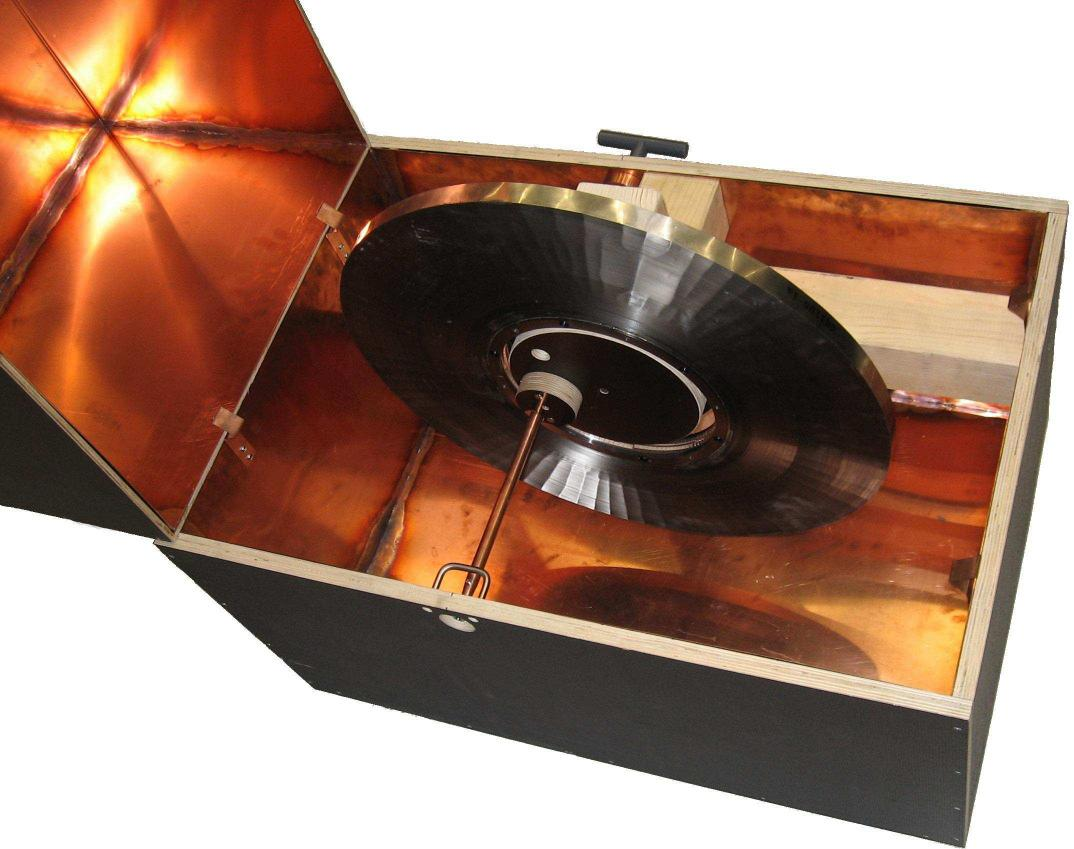
\includegraphics[width=0.5\textwidth]{BoxMitRKCite}
		\caption{Ge\"offnete Testbox mit eingeh\"angtem Ringkern.~\cite{harzheim2016modeling}}
		\label{fig:leereBox}
\end{figure}
F\"ur die ersten Kurzschlussversuche wurden im Test einfache Kupferdr\"ahte mit L\"usterklemmen verwendet. Die Kupferdr\"ahte sind isoliert, sodass diese keinen Kontakt zum Ringkern herstellen. Lediglich die Enden in den Klemmen wurden abgeschliffen, um einen Kontakt herzustellen. Diese Kupferdr\"ahte lassen sich problemlos durch die Bohrungen an der Innenseite des Ringkerns (siehe Abbildung~\ref{fig:innenKern}) f\"uhren, was in Position zumindest an der Innenseite fixiert.
\par
\begin{figure}[htb]
		\centering
		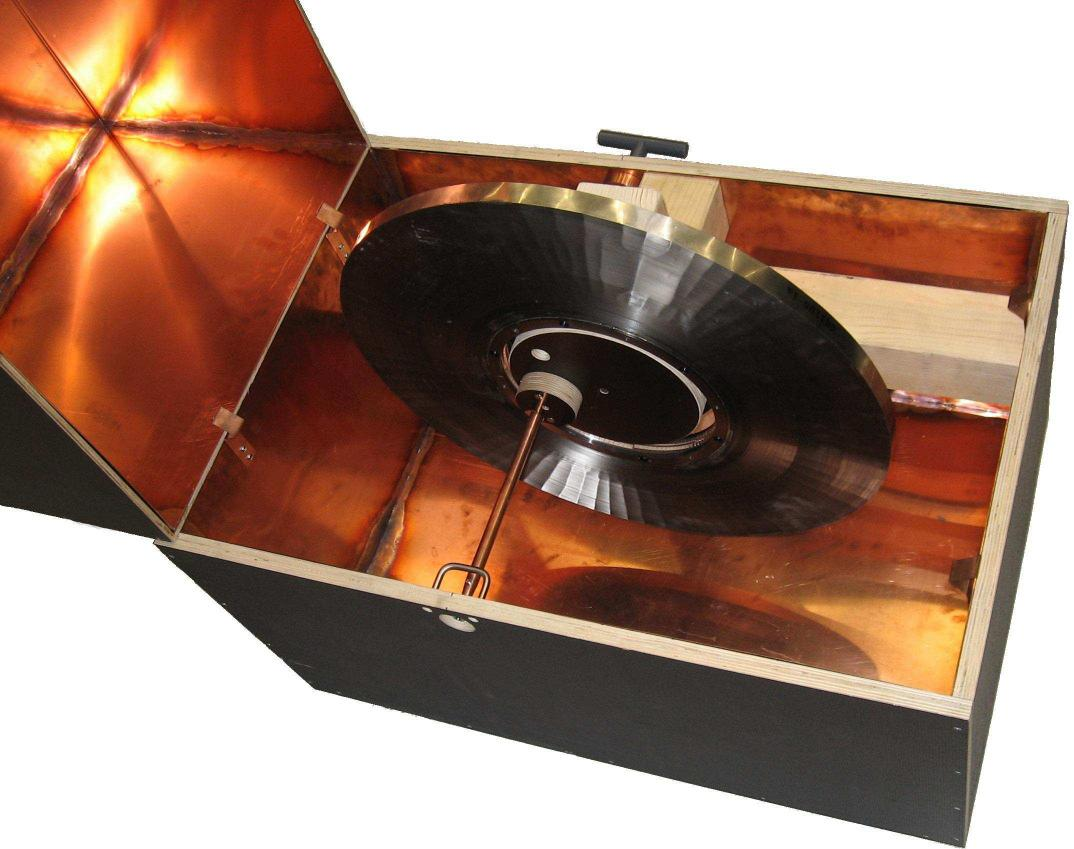
\includegraphics[width=0.5\textwidth]{BoxMitRKCite}
		\caption{Kurzschlusswicklung um den Ringekern mittels eines Drahtes, dessen Enden mit einer L\"usterklemme verbunden sind.}
		\label{fig:innenKern}
\end{figure}
\textbf{???BILD HIER EINFÜGEN}


% \newpage



\subsection{Modifikation}
Um reproduzierbare Messungen durchf\"uhren zu k\"onnen sind mehrere Anforderungen an den Aufbau der Testbox zu stellen. Zun\"achst muss die M\"oglichkeit bestehen, den Magnetic Alloy Ringkern in die Testbox einzubringen, sodass sich dieser bei jeder Messung an der gleichen Position befindet. Des weiteren ist eine M\"oglichkeit zu schaffen, bei der die Kurzschl\"usse an festgelegten  Stellen um den Ringkern zu f\"uhren sind, ohne dass diese den Kern dabei ber\"uhren. Um das zu erreichen wurden mehrere \"Uberlegungen angestellt.
\par
Zum einen Muss eine Ma\ss{}genaue Halterung f\"ur den Ringkern angebracht werden. Dar\"uber hinaus sollte die Halterung einen Anschlag besitzen, um die Position sicher zu stellen. Abbildung~\ref{fig:BoxKreuzPolygon} zeigt die \"Uberarbeitete Halterung. Das Holzkreuz im hinteren Teil der Halterung ragt einige Millimeter \"uber den Rand des Polygon-Rings hinaus, sodass dort ein sicherer Anschlag entsteht. Der Polygon-Ring entspricht mit dem Aus\ss{}enradius von $\SI{129}{\milli\meter}$ mit leichter Toleranz zur besseren Montage dem ben\"otigten Innenradius des Ringkerns von $\SI{130}{\milli\meter}$.


\newpage


\begin{figure}[htb]
	\centering
	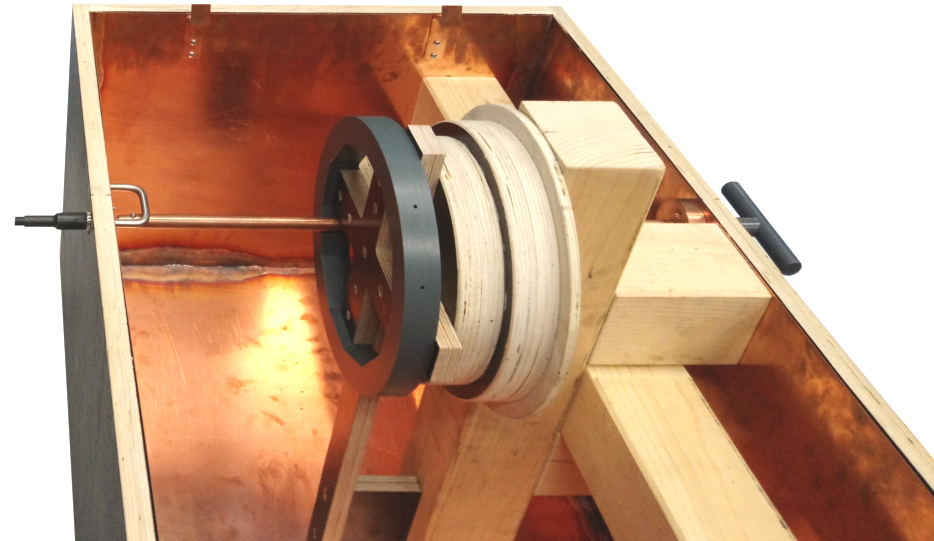
\includegraphics[width=0.65\textwidth]{BoxKreuzPolygon}
	\caption{Halterung aus einem Polygon, welches auf ein Holzkreuz aufgesetzt wurde mit sichtbarem Anschlag.}
	\label{fig:BoxKreuzPolygon}
\end{figure}
\par
Wie erw\"ahnt besitzt die Halterung auf der Innenseite einen Polygonzug. Durch diesen Polygonzug k\"onnen Kurzschlussb\"ugel reproduzierbar an immer gleichen Positionen platziert werden. Dazu wurden an den Fl\"achenmittelpunkten der inneren Polygonfl\"achen Bohrungen mit einem M4 Gewinde vorgesehen, an dem Kurzschl\"usse montiert werden k\"onnen. Abbildung~\ref{fig:BoxKreuzPolygonRK} zeigt den Polygonzug mit montiertem Ringkern.



% \newpage



\begin{figure}[htb]
	\centering
	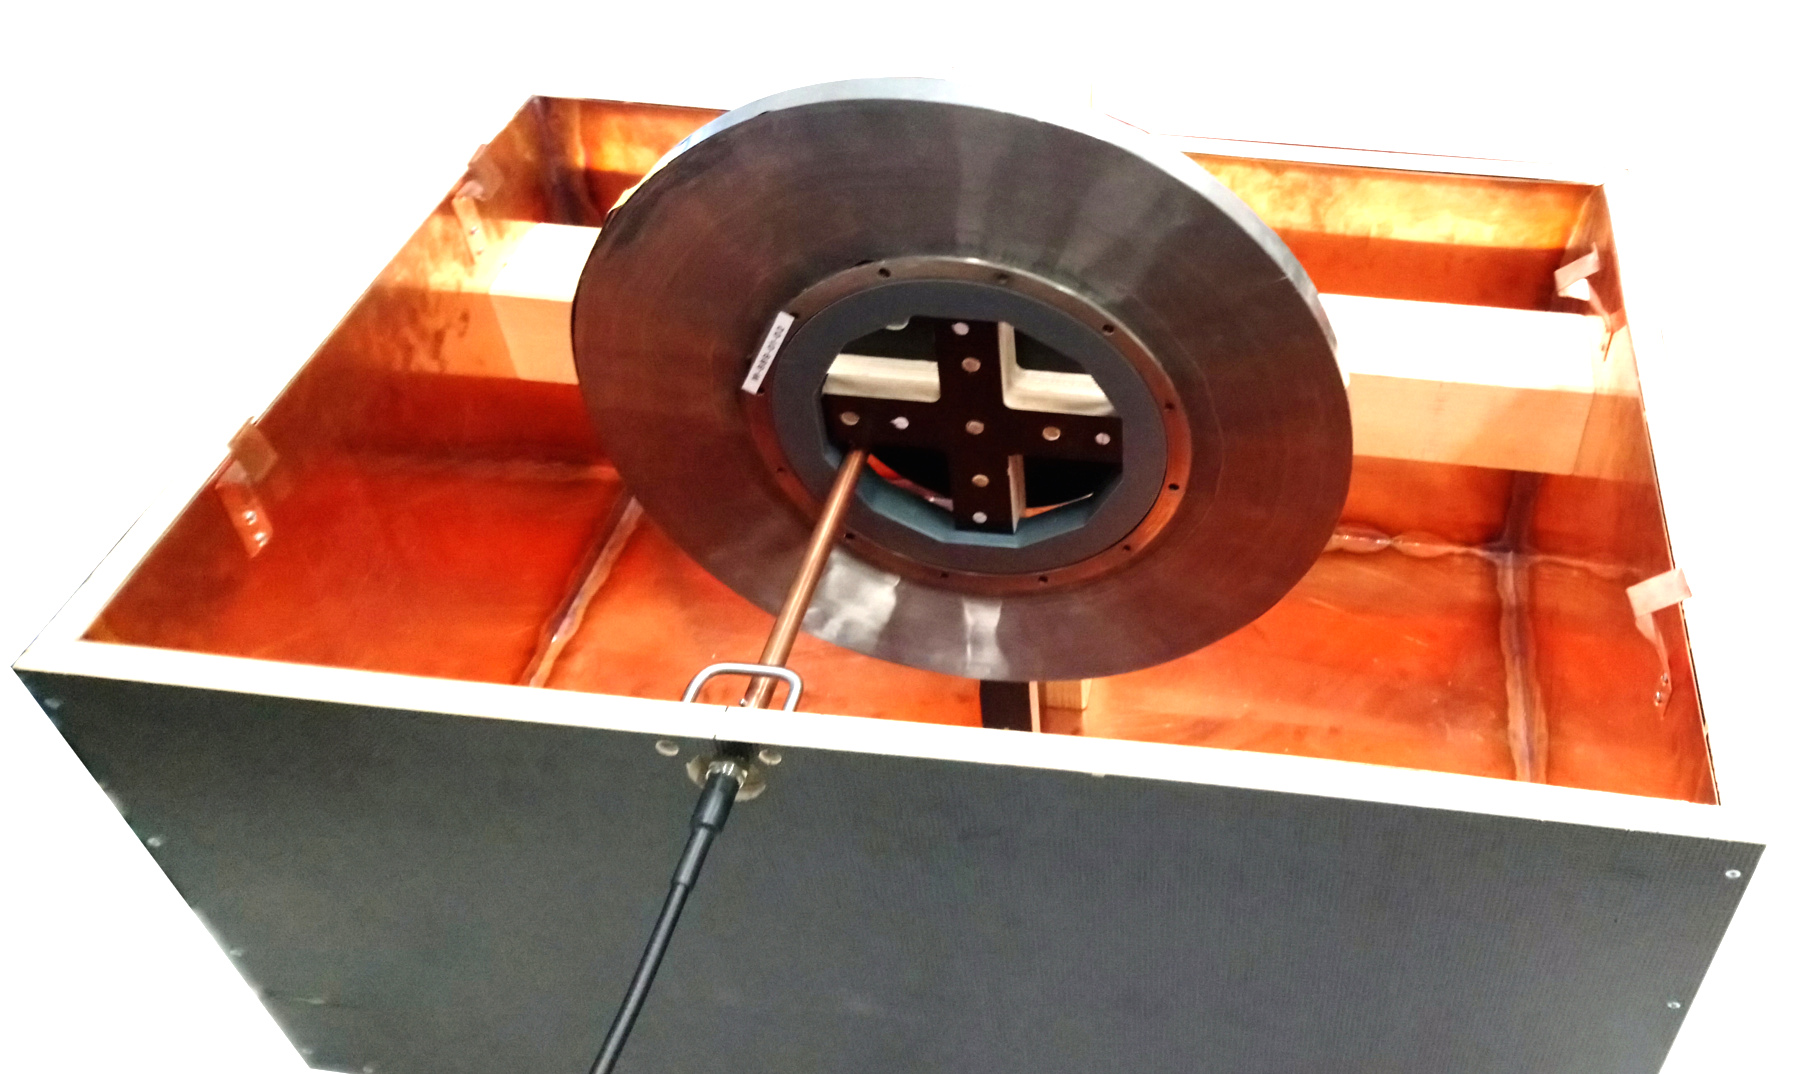
\includegraphics[width=0.85\textwidth]{BoxKreuzPolygonRK}
	\caption{Eingebrachter Ringkern auf der Halterung bestehend aus einem Polygon, welches auf ein Holzkreuz aufgesetzt wird.}
	\label{fig:BoxKreuzPolygonRK}
\end{figure}


\newpage


Durch die Schraubungen im Polygon wird sicher gestellt, dass Kurzschl\"usse stets an der gleichen Position angebracht werden, unabh\"angig der genauen Form der Kurzschl\"usse. Abbildung~\ref{fig:TZKS} zeigt eine Beispielhafte Kurzschlussschiene.
\par
\begin{figure}[htb]
	\centering
	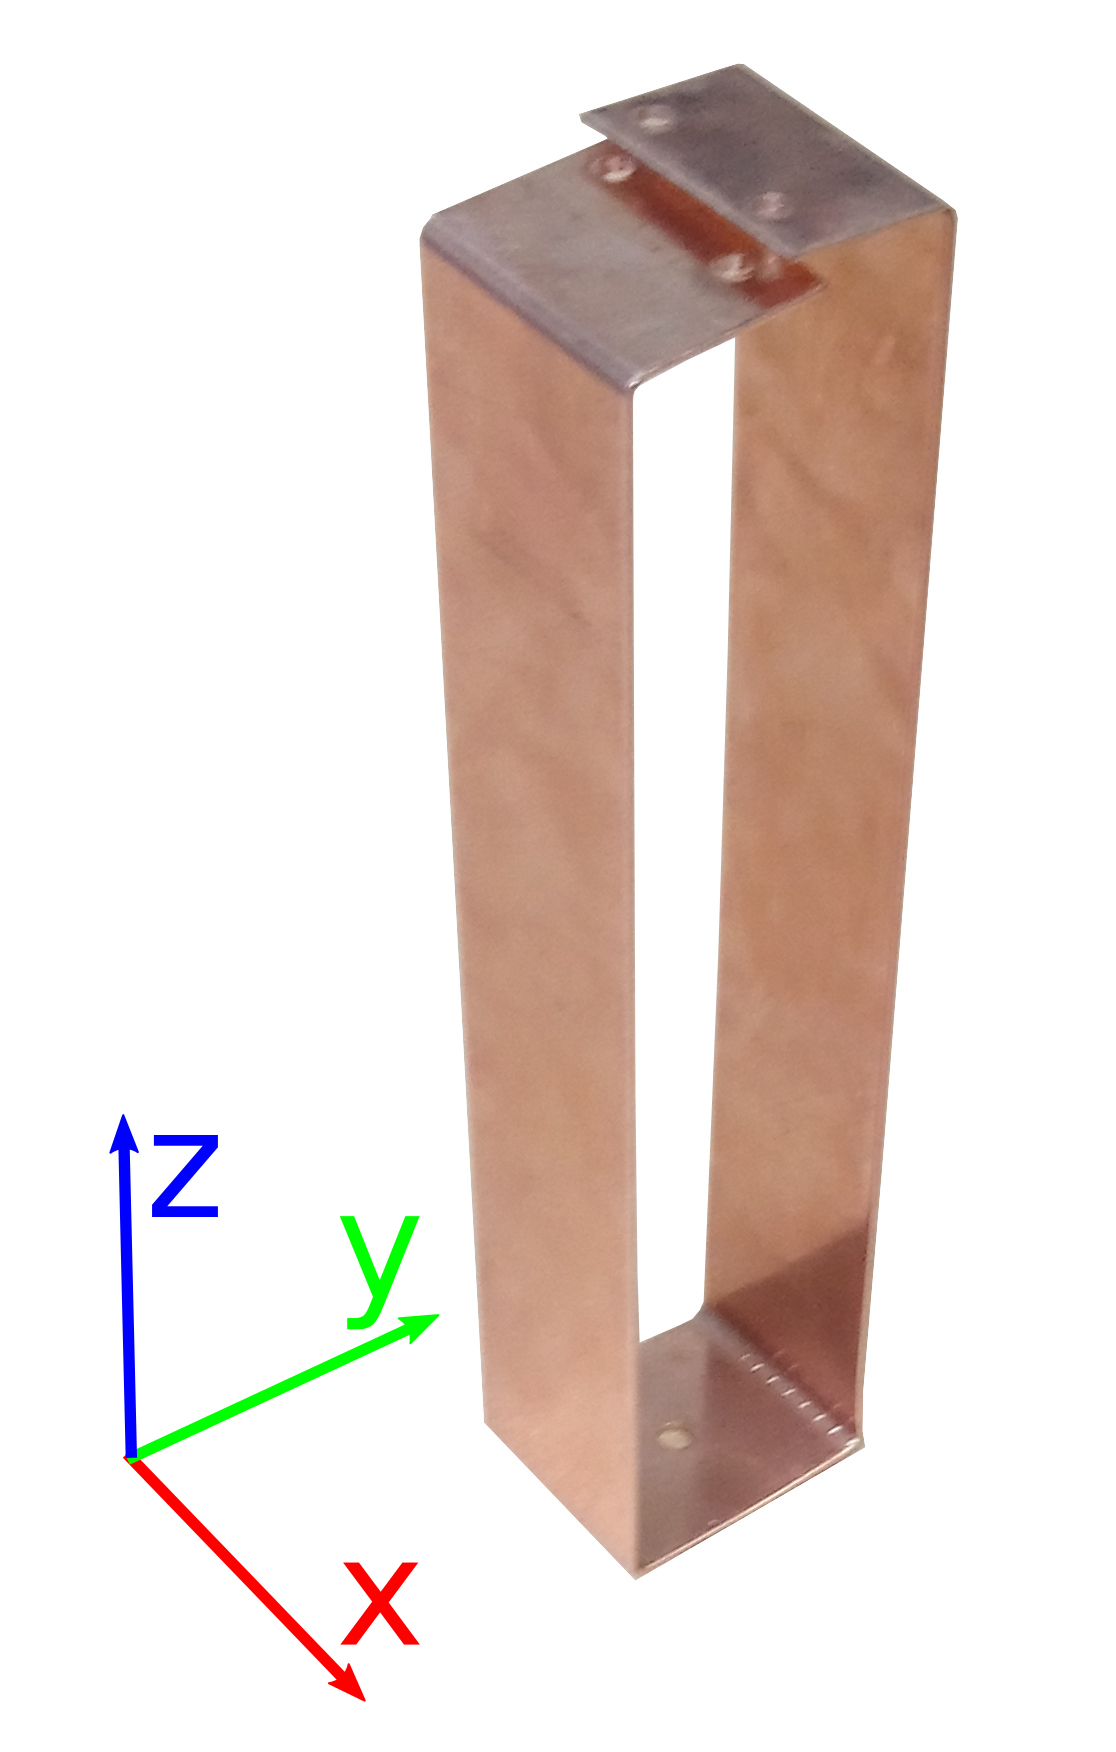
\includegraphics[height=0.4\textwidth]{KS}
	\caption{Kurzschlussschiene mit einer H\"ohe in z-Richtung von $\SI{160}{\milli\meter}$ einer Breite in x-Richtung von $\SI{30}{\milli\meter}$ und einer Blechdicke von $\SI{1}{\milli\meter}$.}
	\label{fig:TZKS}
\end{figure}
Die getesteten Formen der Kurzschl\"usse sind in mehrere Variationsparameter unterteilt:
\begin{itemize}
	\item H\"ohe der Kurzschl\"usse in z-Richtung
	\item Breite der Kurzschl\"usse in x-Richtung
	\item Blechdicke der K\"urzschl\"usse
\end{itemize}
\par
F\"ur die Messung wurde daher eine ganze Reihe an Kurzschlussschienen angefertigt, damit f\"ur jede Form der Schienen unterschiedliche Anzahlen an Kurzschl\"ussen gemessen werden k\"onnen und mehrere Stufen f\"ur jeden Variationsparameter vorhanden sind. Ein Bild aller Kurzschlussschienen ist in Abbildung~\ref{fig:AlleKs} zu sehen.
\par
\begin{figure}[htb]
	\centering
	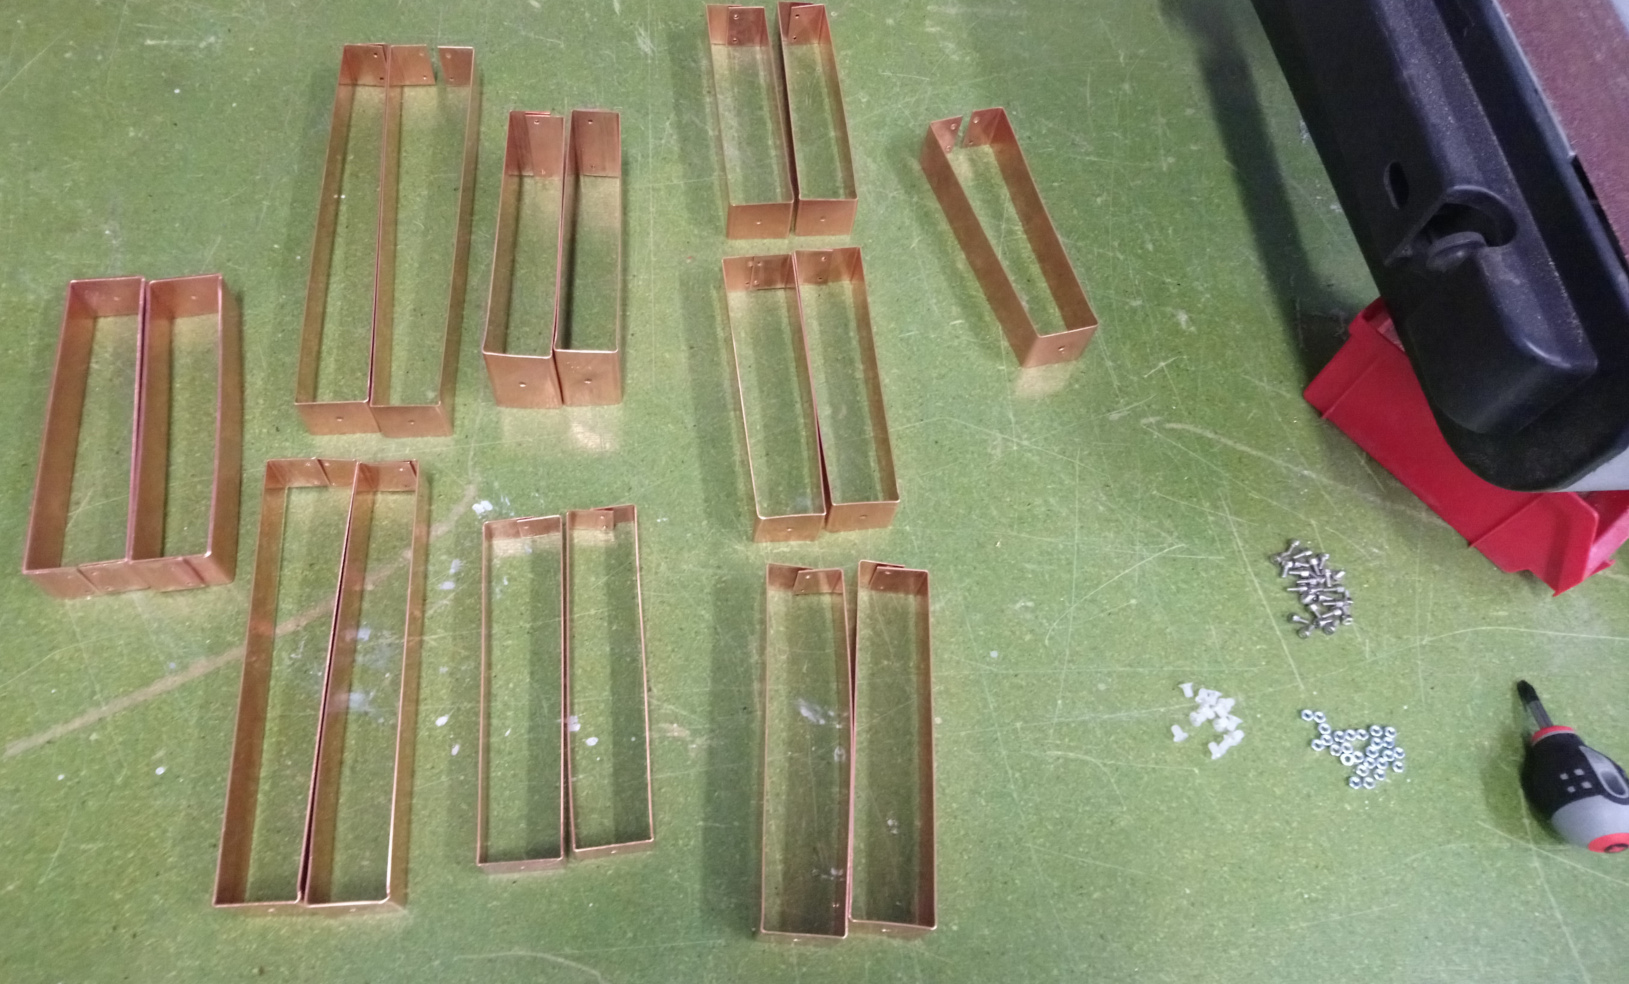
\includegraphics[width=0.65\textwidth]{AlleKs}
	\caption{Alle f\"ur Messungen angefertigte Kurzschlussschienen.}
	\label{fig:AlleKs}
\end{figure}
Insgesamt wurden folgende Kurzschl\"usse angefertigt:
\par
\begin{itemize}
	\item 8x $\SI{160}{\milli\meter}$ H\"ohe in z-Richtung, $\SI{30}{\milli\meter}$ Breite in x-Richtung und $\SI{1}{\milli\meter}$ Blechdicke
	\item 2x $\SI{200}{\milli\meter}$ H\"ohe in z-Richtung, $\SI{30}{\milli\meter}$ Breite in x-Richtung und $\SI{1}{\milli\meter}$ Blechdicke
	\item 2x $\SI{250}{\milli\meter}$ H\"ohe in z-Richtung, $\SI{30}{\milli\meter}$ Breite in x-Richtung und $\SI{1}{\milli\meter}$ Blechdicke
	\item 2x $\SI{160}{\milli\meter}$ H\"ohe in z-Richtung, $\SI{20}{\milli\meter}$ Breite in x-Richtung und $\SI{1}{\milli\meter}$ Blechdicke
	\item 2x $\SI{160}{\milli\meter}$ H\"ohe in z-Richtung, $\SI{50}{\milli\meter}$ Breite in x-Richtung und $\SI{1}{\milli\meter}$ Blechdicke
	\item 2x $\SI{160}{\milli\meter}$ H\"ohe in z-Richtung, $\SI{30}{\milli\meter}$ Breite in x-Richtung und $\SI{2}{\milli\meter}$ Blechdicke
\end{itemize}
Daraus lie\ss{} sich folglich eine Gesamtzahl von 18 Messungen durchf\"uhren. Die Schienen selbst wurden jeweils aus einem l\"anglichen St\"uck Kupferblech gefertigt. Dieses wurde in die vorgesehene Dimension gebogen. Zum schlie\ss{}en der Schienen befinden sich an beiden Enden des Kupferblechs jeweils 2 L\"ocher, welche nach dem Biegen mit Schrauben und Muttern verbunden werden k\"onnen. In der Mitte des Kupferblechs, welche nach dem Biegen auf der Innenseite des Polygons liegt, befindet sich ein Loch mit dem Durchmesser $\SI{4}{\milli\meter}$. Dadurch k\"onnen werden die Schienen dann mittels einer Schraube positionsgenau auf die vorgesehenen Gewinde an den Polygonfl\"achen montiert.
	
\chapter{Simulation}\label{chap:simulation}
	\label{ch:sim}
        \section{Motivation}
    Um die Einflüsse verschiedener Kurzschlussanordnungen und -ausführungen schon im Vorfeld abschätzen zu können und ein erstes Gefühl für den Einfluss der Kurzschlüsse zu bekommen, wurde die Testanordnung zunächst ausgiebig mit der Simulationssoftware CST simuliert.\\
    Die Simulationen dienten als Vorbereitung, um bei den Messungen präziser vorgehen zu können und gezielt Messungen durchzuführen. Zuletzt wurden die Simulationsergebnisse dann mit den Messergebnissen gegenübergestellt und verglichen, um deren Richtigkeit zu überprüfen.
    
    \section{Modellierung}
        \subsection{Bestehendes Testbox- und Ringkernmodell}
        Als Grundlage für die Simulation der Testbox und des Ringkerns dient das Simulationsmodell von Testbox inklusive Ringkern aus der Bachelorarbeit von Denys Bast \citep{bast2017ba}.\\
        Die Außenwände der Testbox sind geometrisch sehr genau den Abmessungen des realen Teststandes entsprechend modelliert, als Material wird hierfür reines Kupfer verwendet, wie es in der Datenbank von CST zu finden ist. Die leere Box ist in Abbildung~\ref{fig:BoxCST} dargestellt.
        
            \begin{figure}[htb]
                \centering
                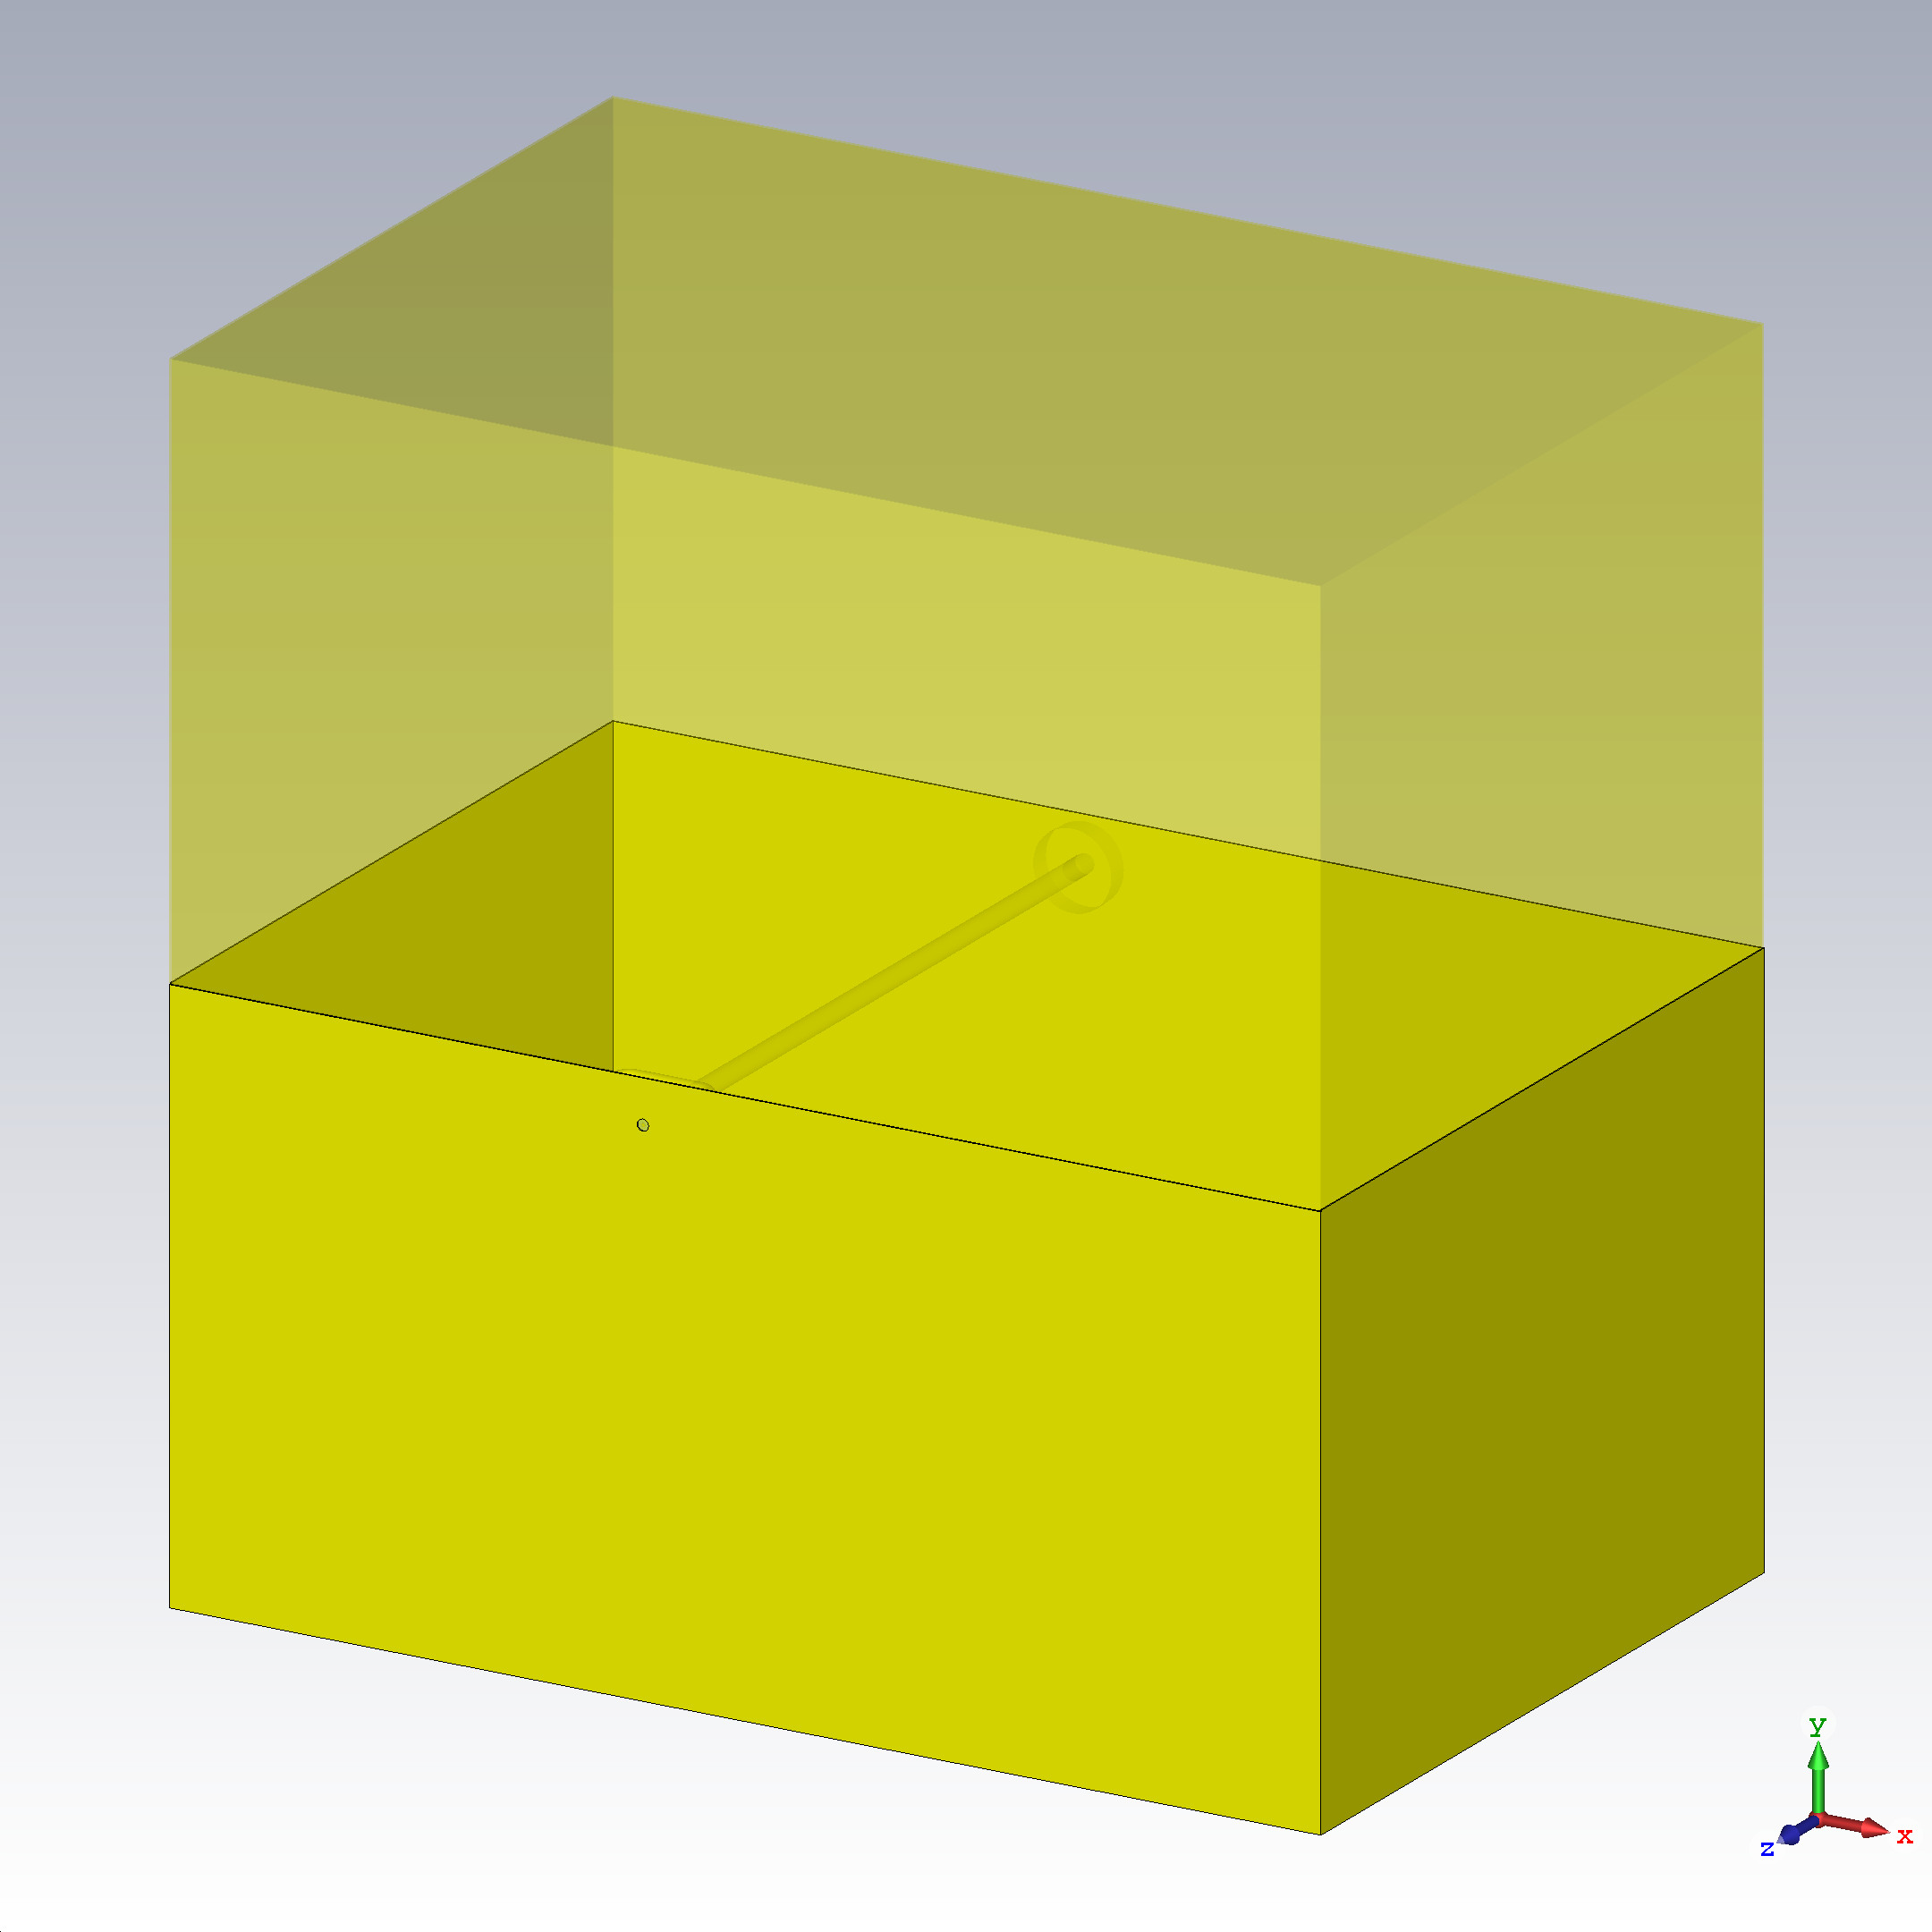
\includegraphics[height=0.4\textwidth]{./Simulation/BoxWaende2.png}
                \caption{Modell der Testbox in CST}
                \label{fig:BoxCST}
            \end{figure}
        In Abbildung~\ref{fig:InnenleiterCST} ist die Signaleinkopplung der Testbox zu sehen.
        Diese ist als Hohlzylinder aus Kupfer modelliert und geometrisch genau am realen Vorbild orientiert. Die Stange ist an der hinteren Wand elektrisch mit der Box verbunden und an der Vorderseite durch einen elektrisch nicht leitfähigen Ring aus Polyethylen (PE, CST Datenbank) von der Box isoliert. Hierdurch wird erreicht, dass die Stange als Hin- und die Boxaußenwände als Rückleiter für Signale dienen. Der Übergang zwischen Testbox, PE und Stange ist planar ausgeführt, um einen Signalport für die Simulation darzustellen.
        
            \begin{figure}[htb]
                \centering
                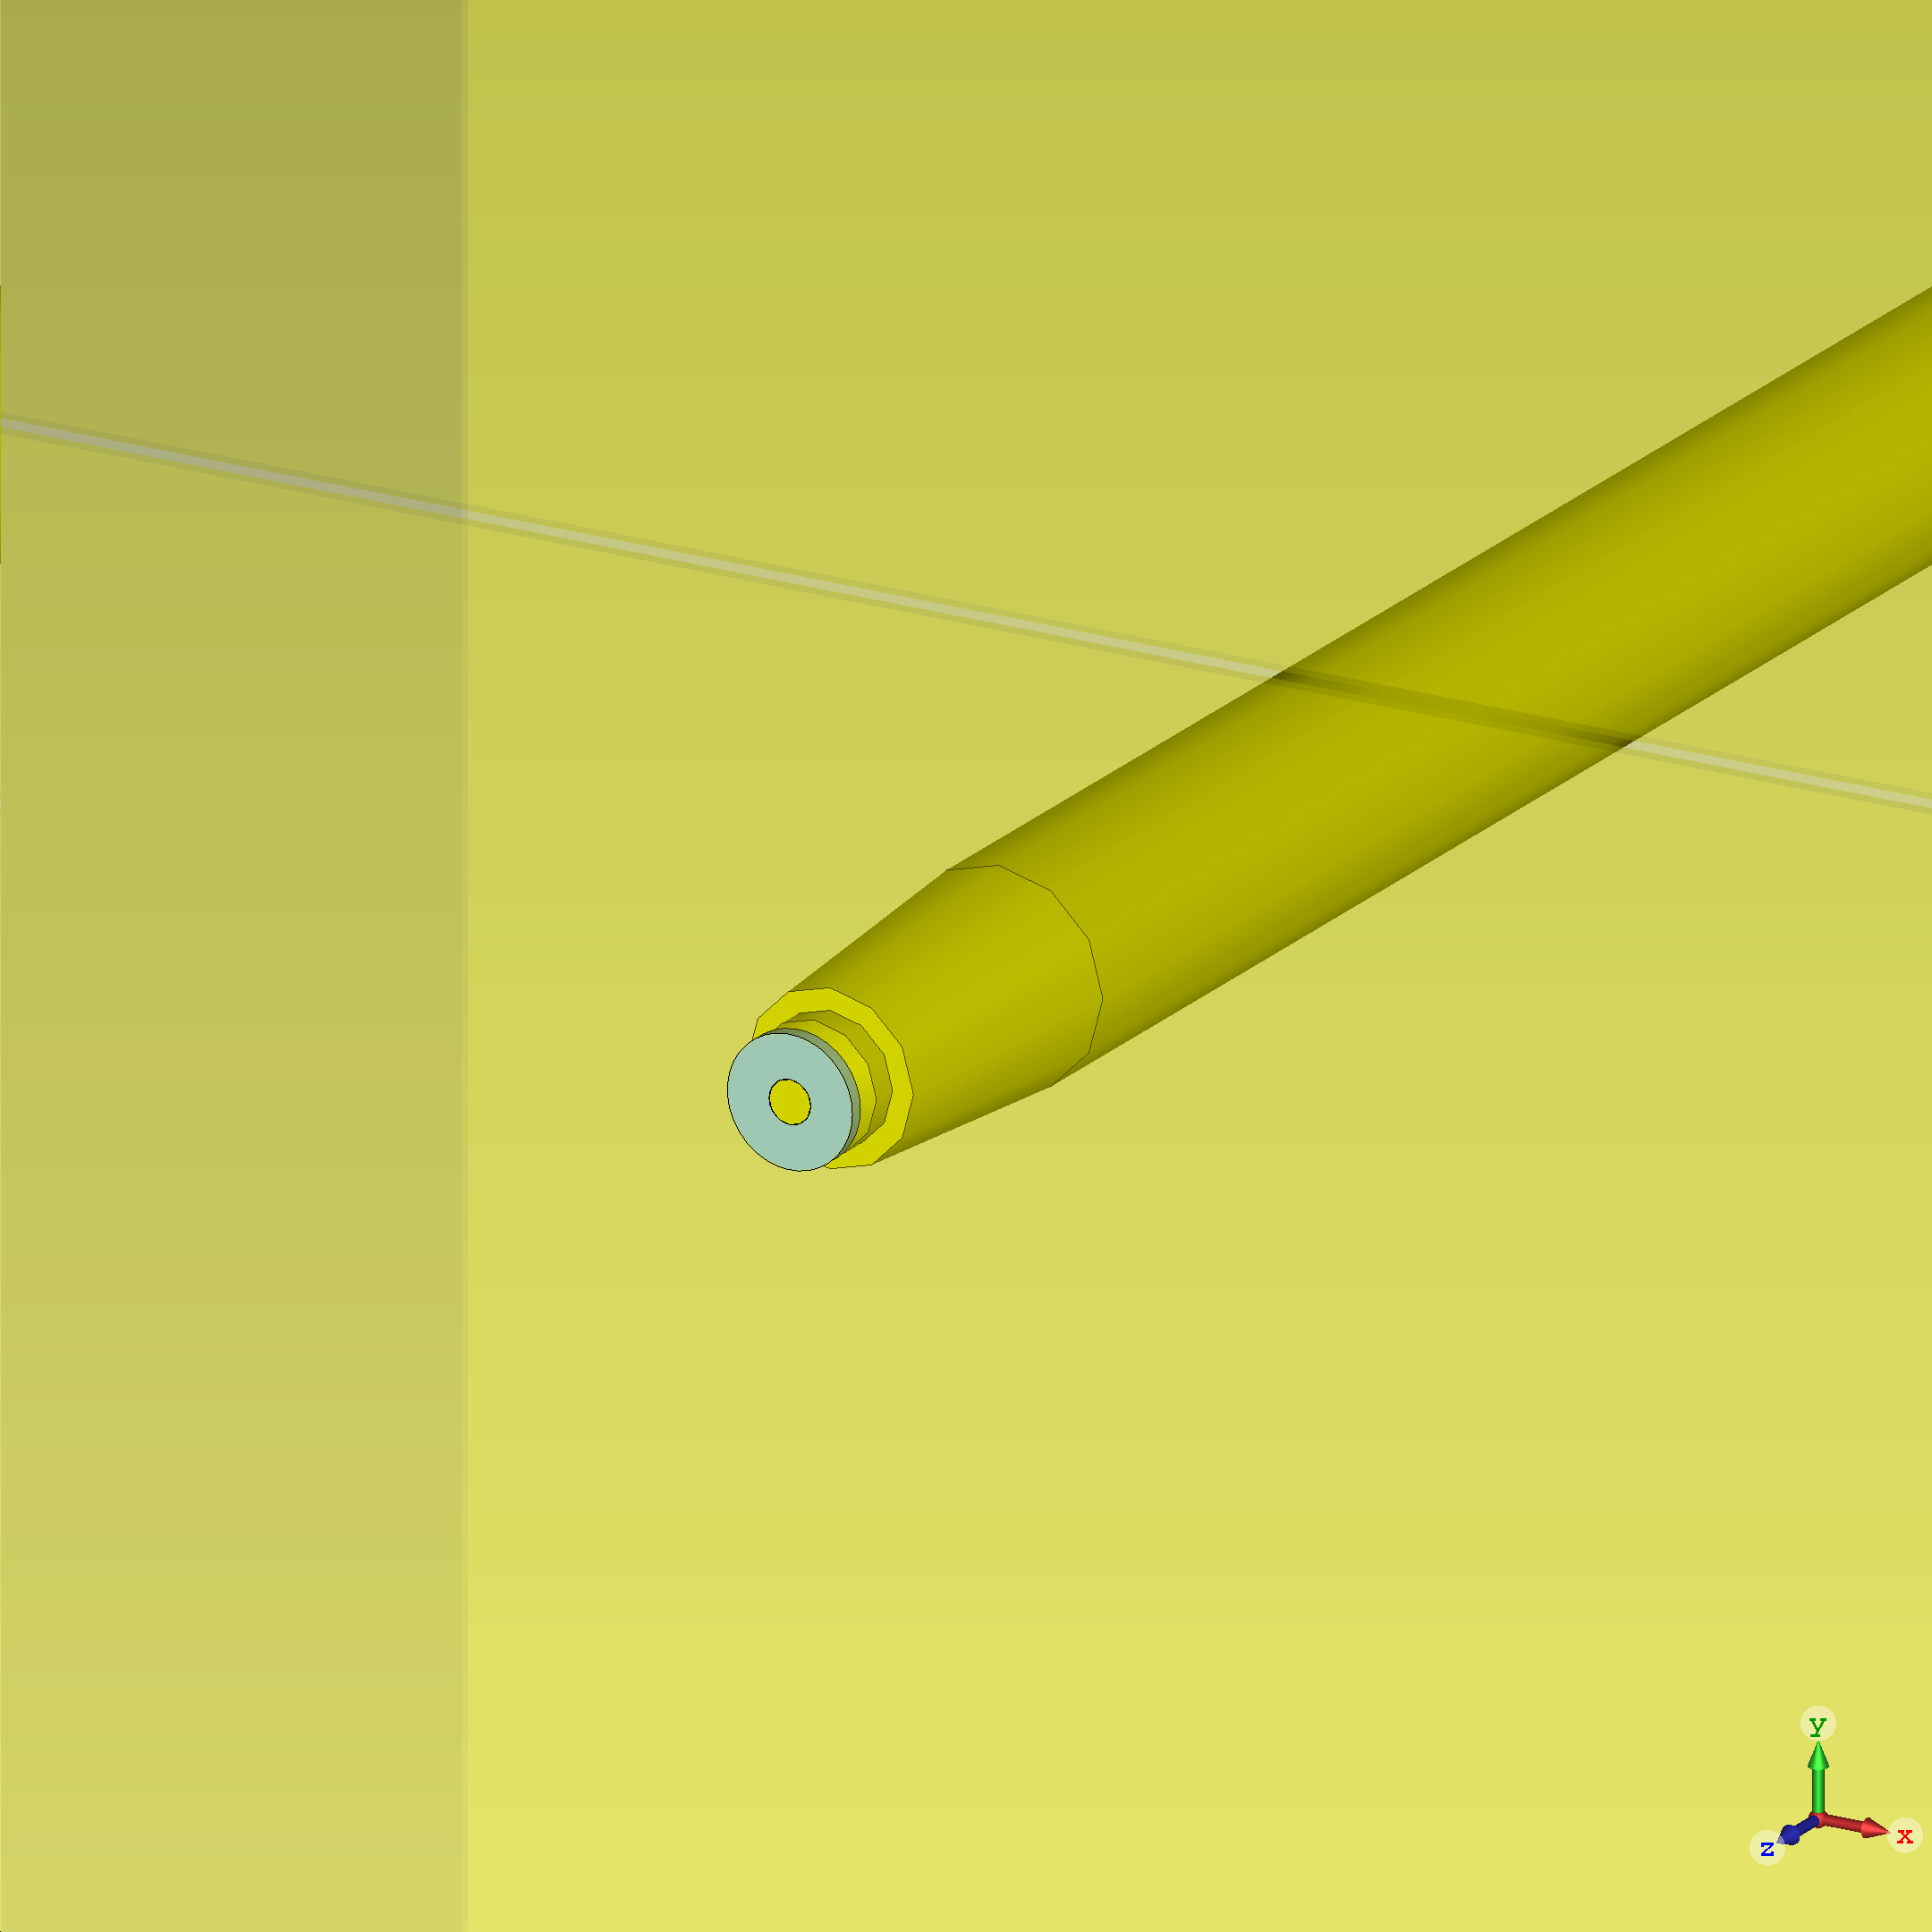
\includegraphics[height=0.4\textwidth]{./Simulation/InnenleiterPE.png}
                \caption{Modell der Einkopplungsstange mit elektrischer Isolation}
                \label{fig:InnenleiterCST}
            \end{figure}
        
        Der Ringkern ist als einfacher Hohlzylinder mit den geometrischen Abmessungen seines realen Vorbild modelliert. Dem realen Aufbau entsprechend ist er zentral im Testboxmodell, allerdings freischwebend, ohne die hölzerne Halterung, modelliert.\\
        Ein grundlegender Aspekt der Arbeit von Denys Bast~\citep{bast2017ba} ist, die magnetische Permeabilität des Ringkernmaterials in der Simulation mit dem realen Material in Übereinstimmung zu bringen. Die dabei gewonnenen Daten wurden übernommen.
        
            \begin{figure}[htb]
                \centering
                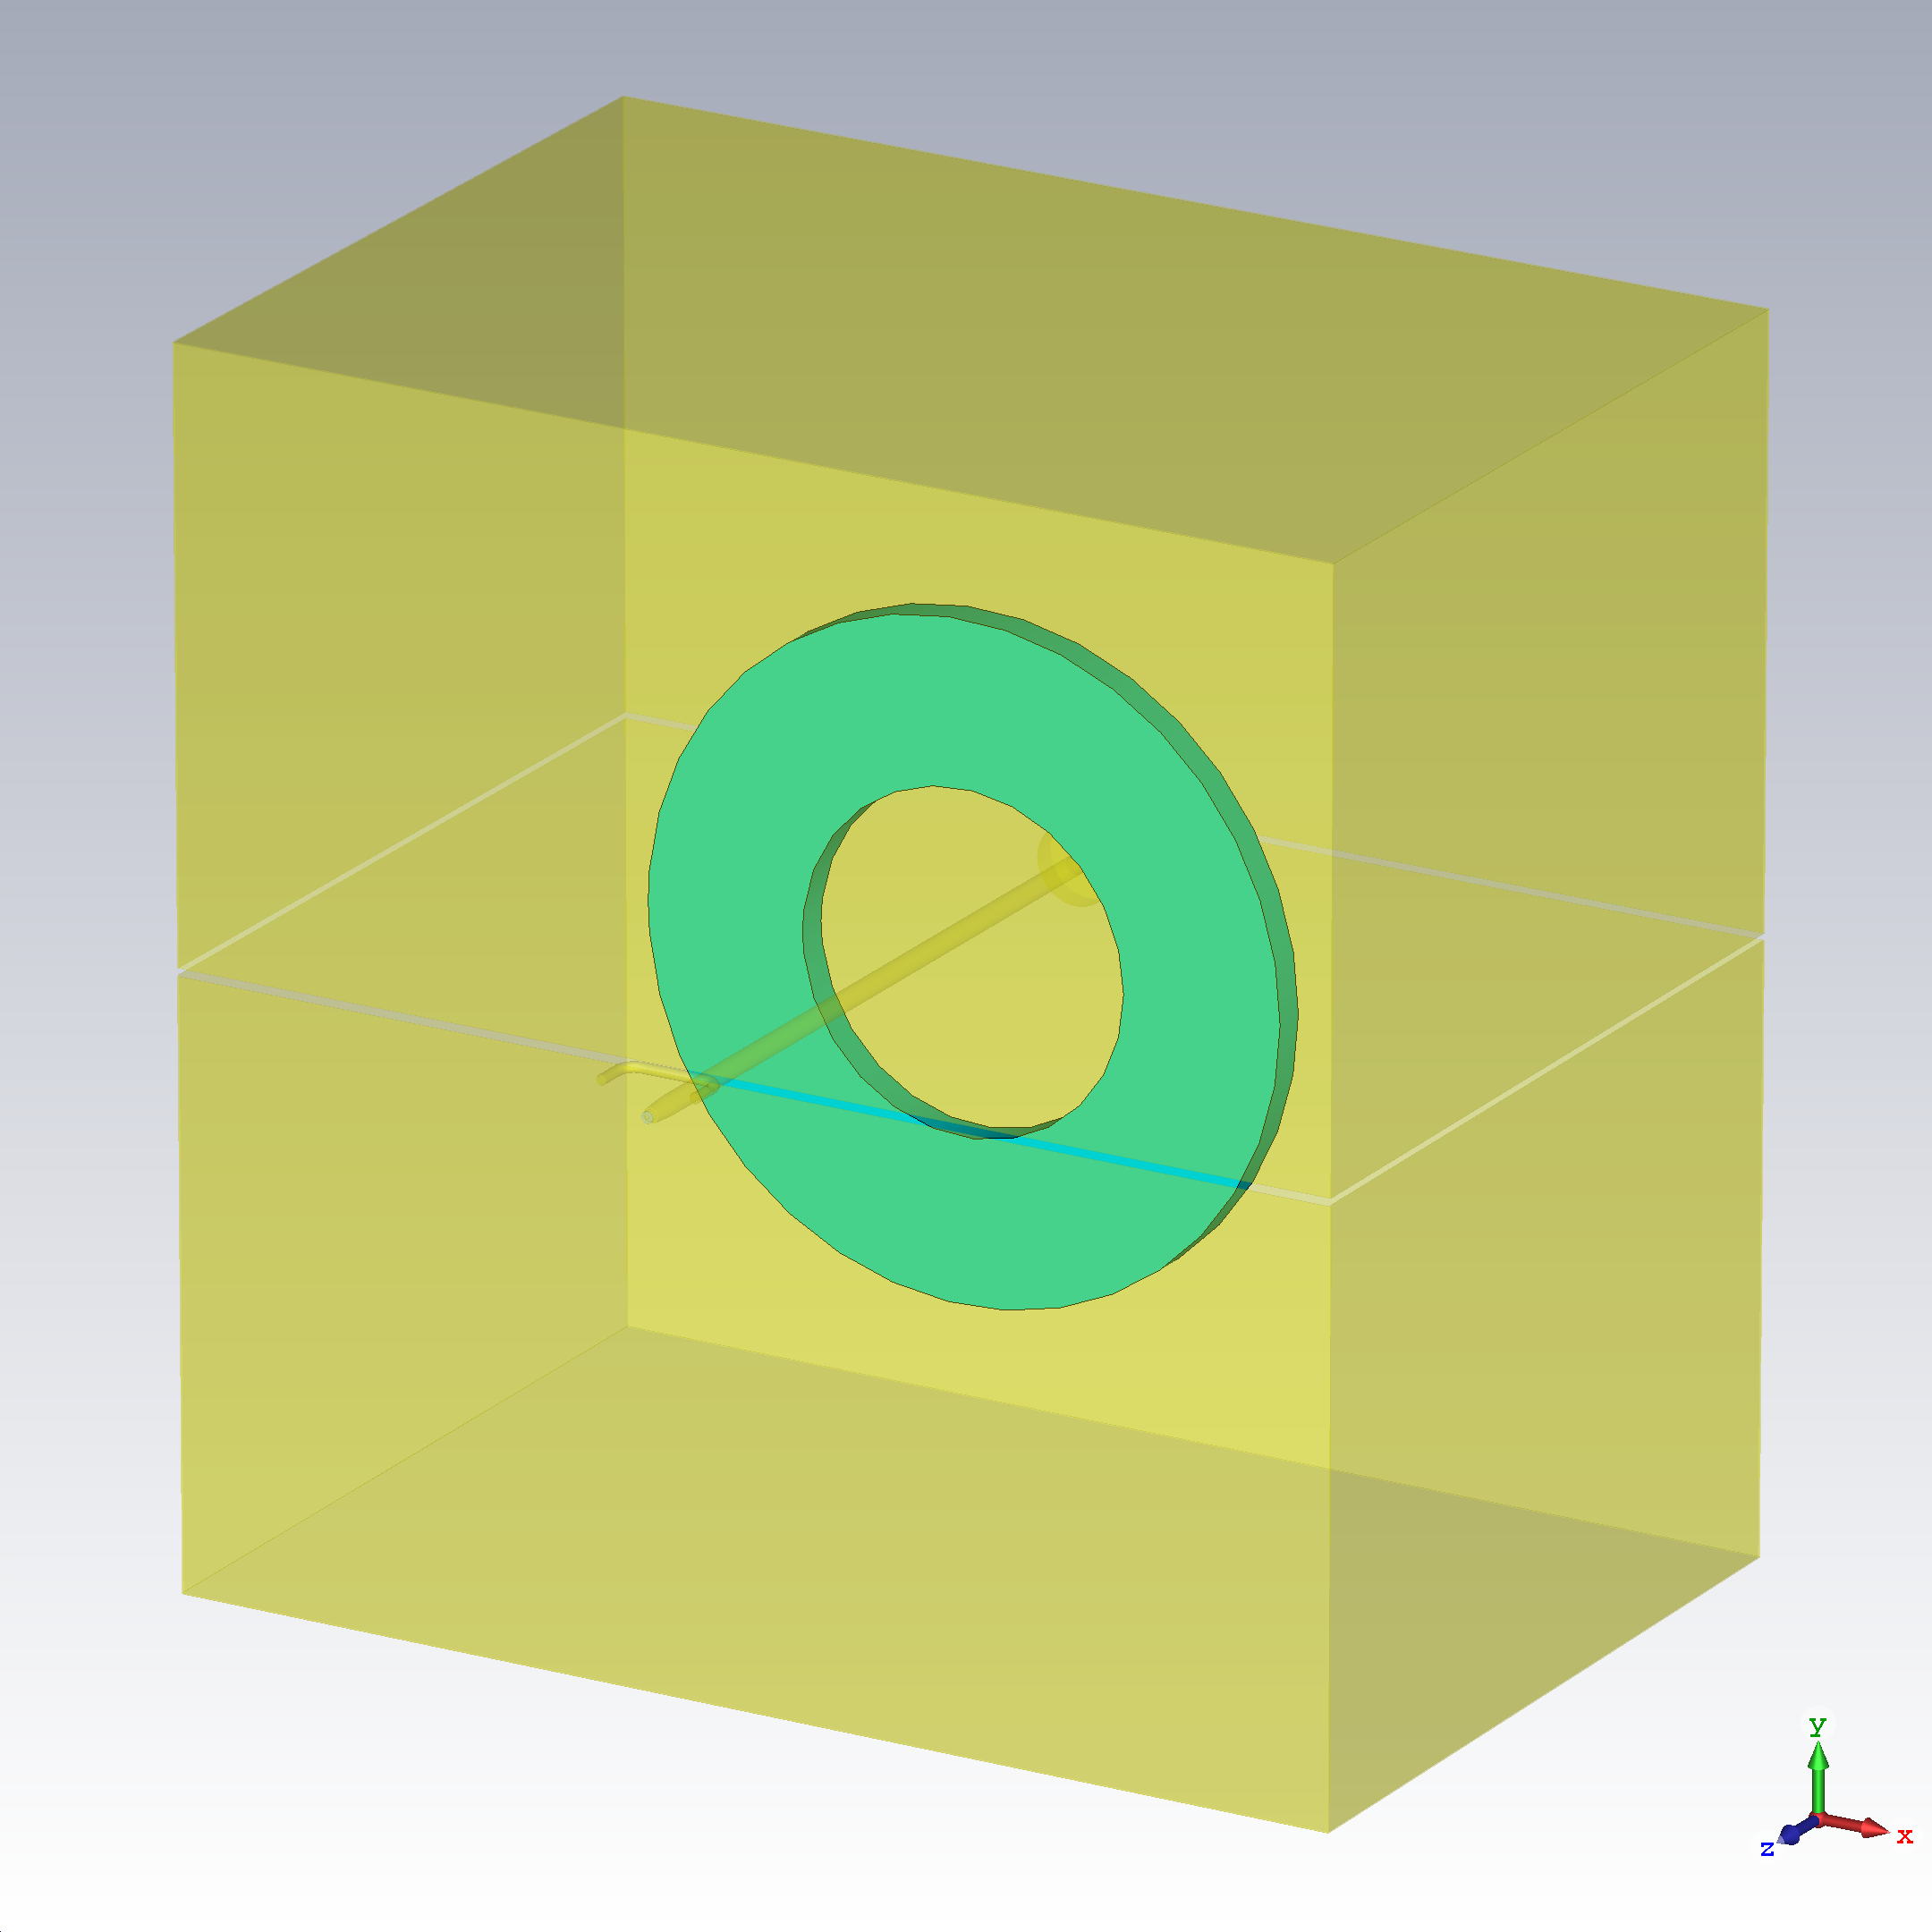
\includegraphics[height=0.4\textwidth]{./Simulation/BoxRK.png}
                \caption{Gesamtdarstellung der Modellierung von Testbox und Ringkern nach Denys Bast~\citep{bast2017ba}}
                \label{fig:BoxRKCST}
            \end{figure}
        
        Abbildung~\ref{fig:BoxRKCST} bildet den modellierten Aufbau der Testbox mit Ringkern ab, wie er in \citep{bast2017ba} beschrieben wird.

        \subsection{Kurzschlüsse}
        Die für die Parameteranalyse dieser Arbeit benötigten Kurzschlüsse sind in CST in verschiedenen, komplexen Ausführungen modelliert.\\
        Die erste Version stellt ein einfacher, ellipsenförmiger Torus dar, wie er in Abbildung~\ref{fig:KSCST}\subref{subfig:V1} abgebildet ist. Als Material für die Simulation wird Kupfer aus der Datenbank von CST verwendet.\\
        Die in Kapitel~\ref{sec:testbox} beschriebenen Verbesserungen der Kurzschlüsse für eine erhöhte Reproduzierbarkeit der Messungen, sind so in CST modelliert. Abbildung~\ref{fig:KSCST}\subref{subfig:V2} zeigt die Umformung des einfachen Torus zu einem schienenförmigen Kurzschluss. Die finale Version, die letztlich für die Messungen benutzt wurde, ist in Abbildung~\ref{fig:KSCST}\subref{subfig:V3} zu sehen. Die einfache Kupferschiene ist geometrisch an die verwendeten Kurzschlüsse angepasst und um die Verbindungsschrauben erweitert.
        
            \begin{figure}[htb]
                \centering
                \subfloat[Version 1]{
                    \label{subfig:V1}
                    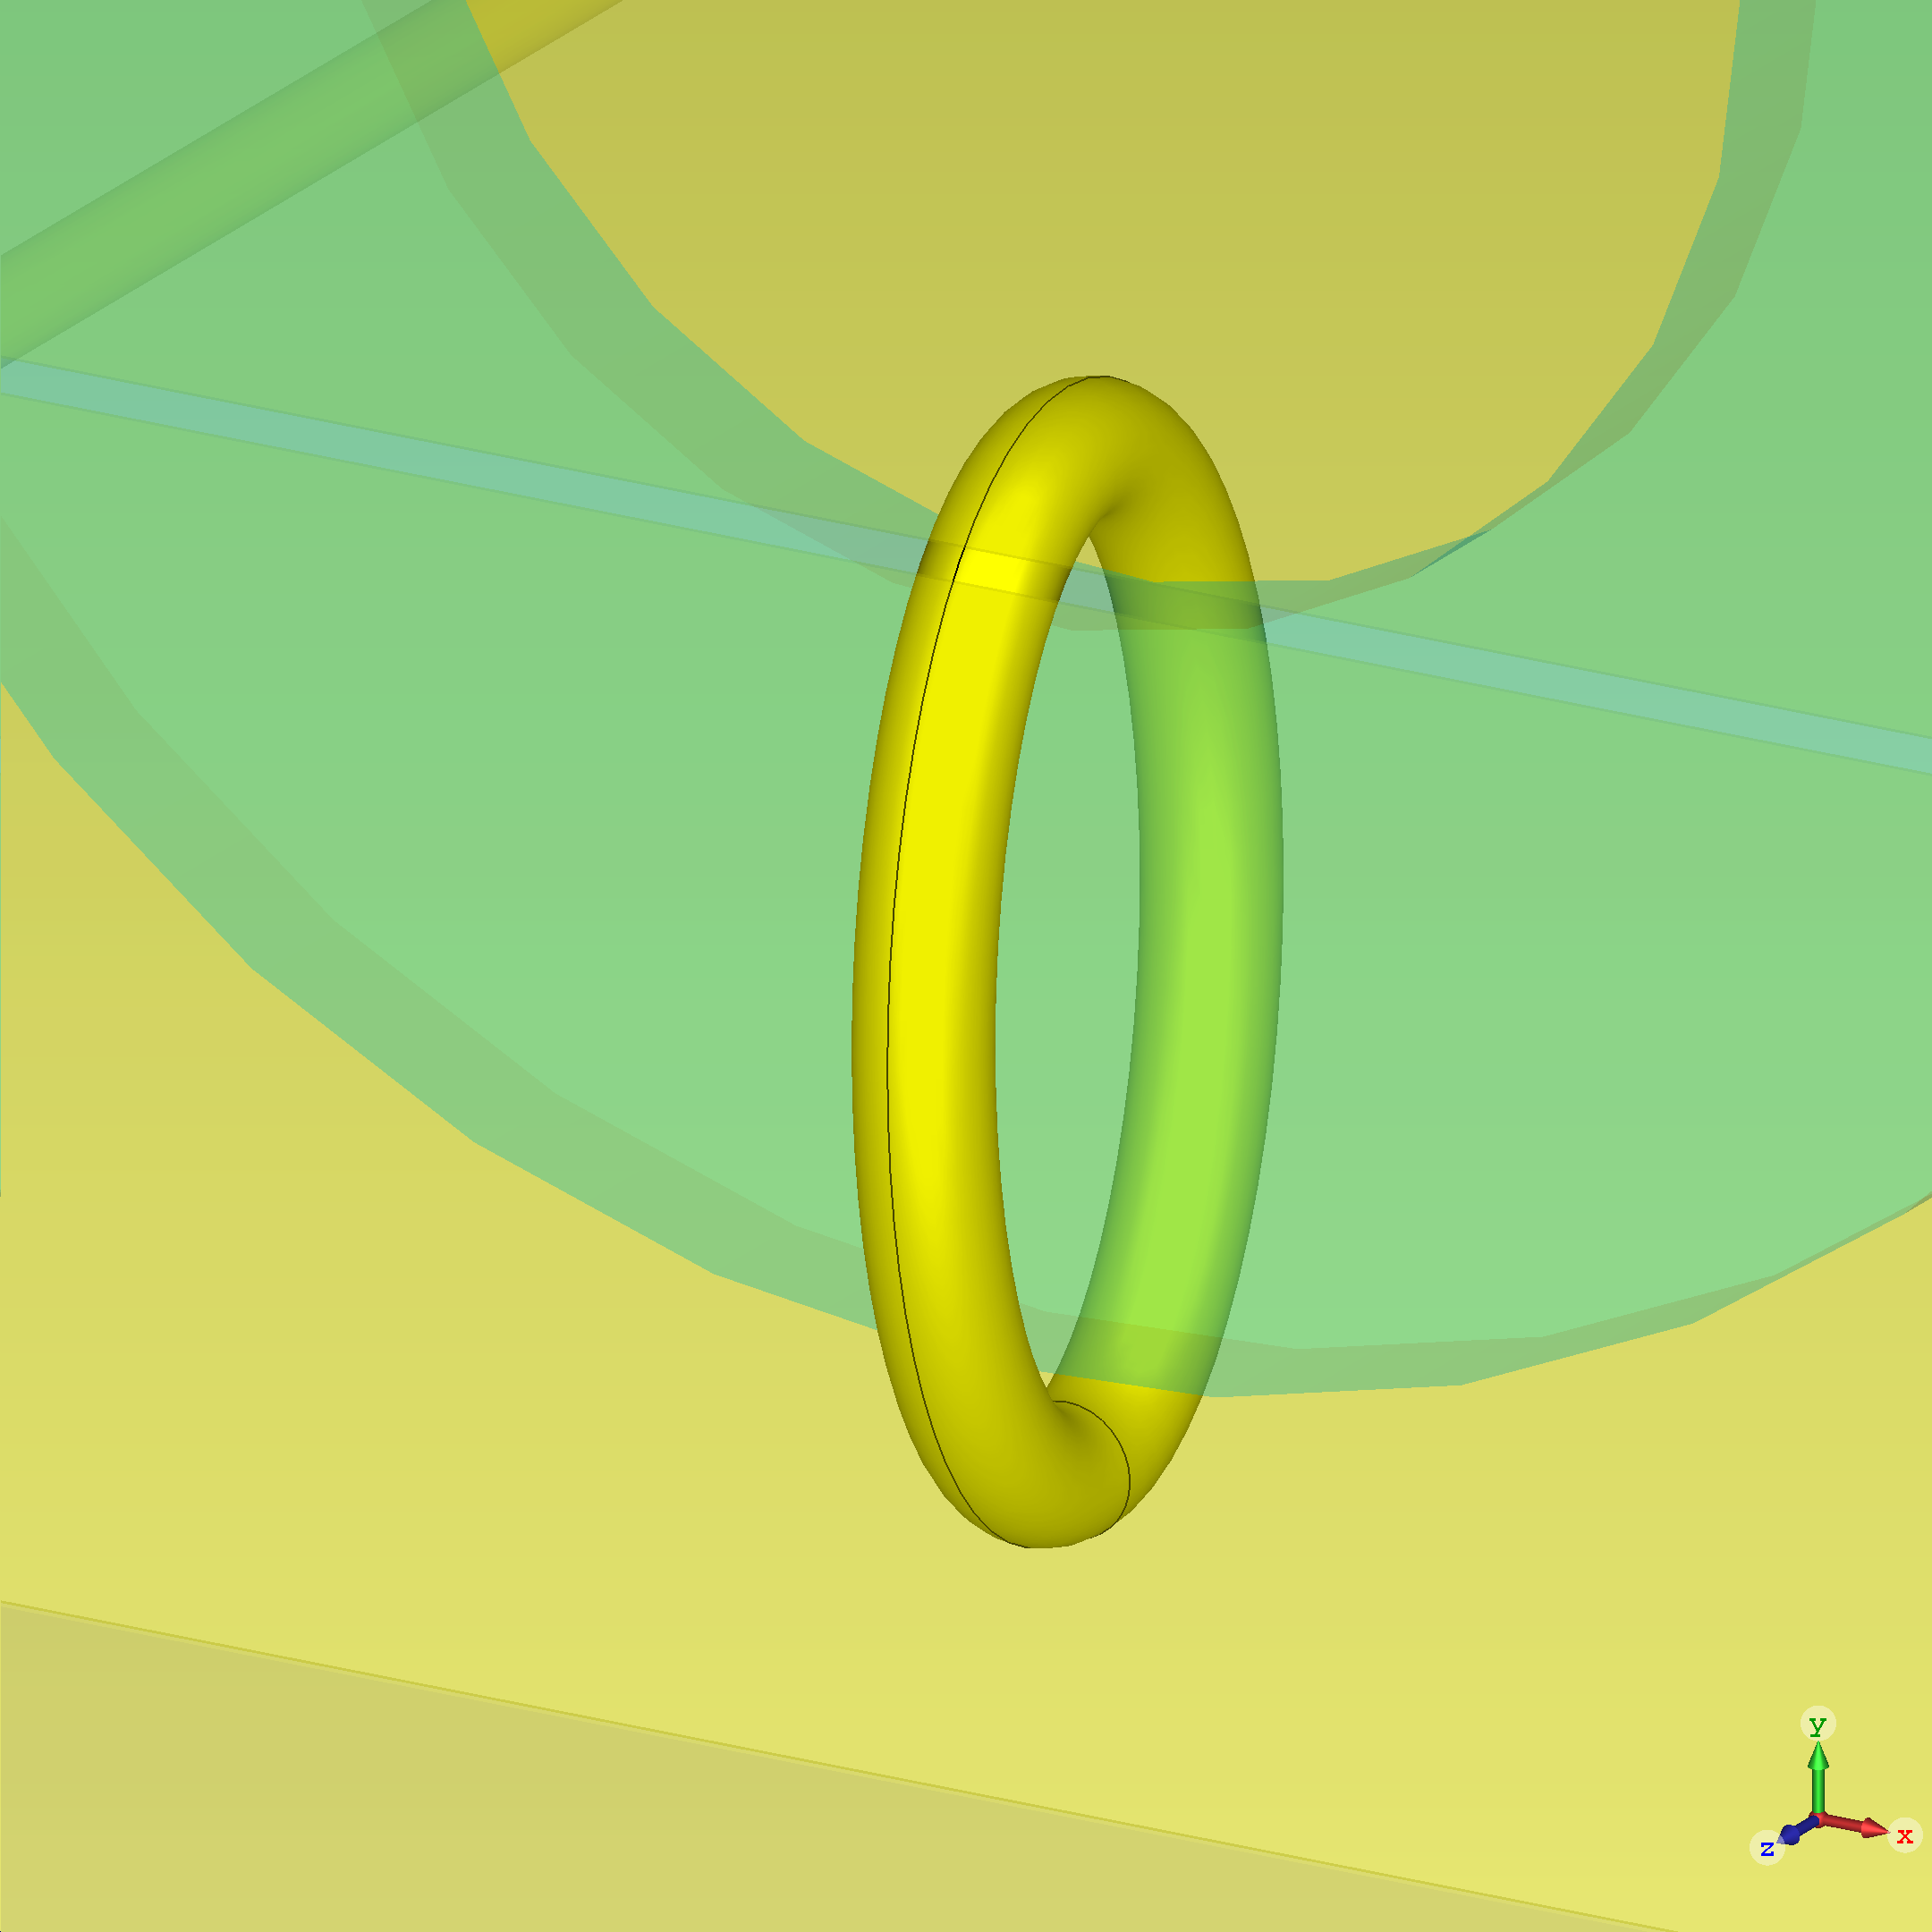
\includegraphics[height=0.3\textwidth]{./Simulation/KSV1Torus.png}}
                \hspace{0.01\textwidth}
                \subfloat[Version 2]{
                    \label{subfig:V2}
                    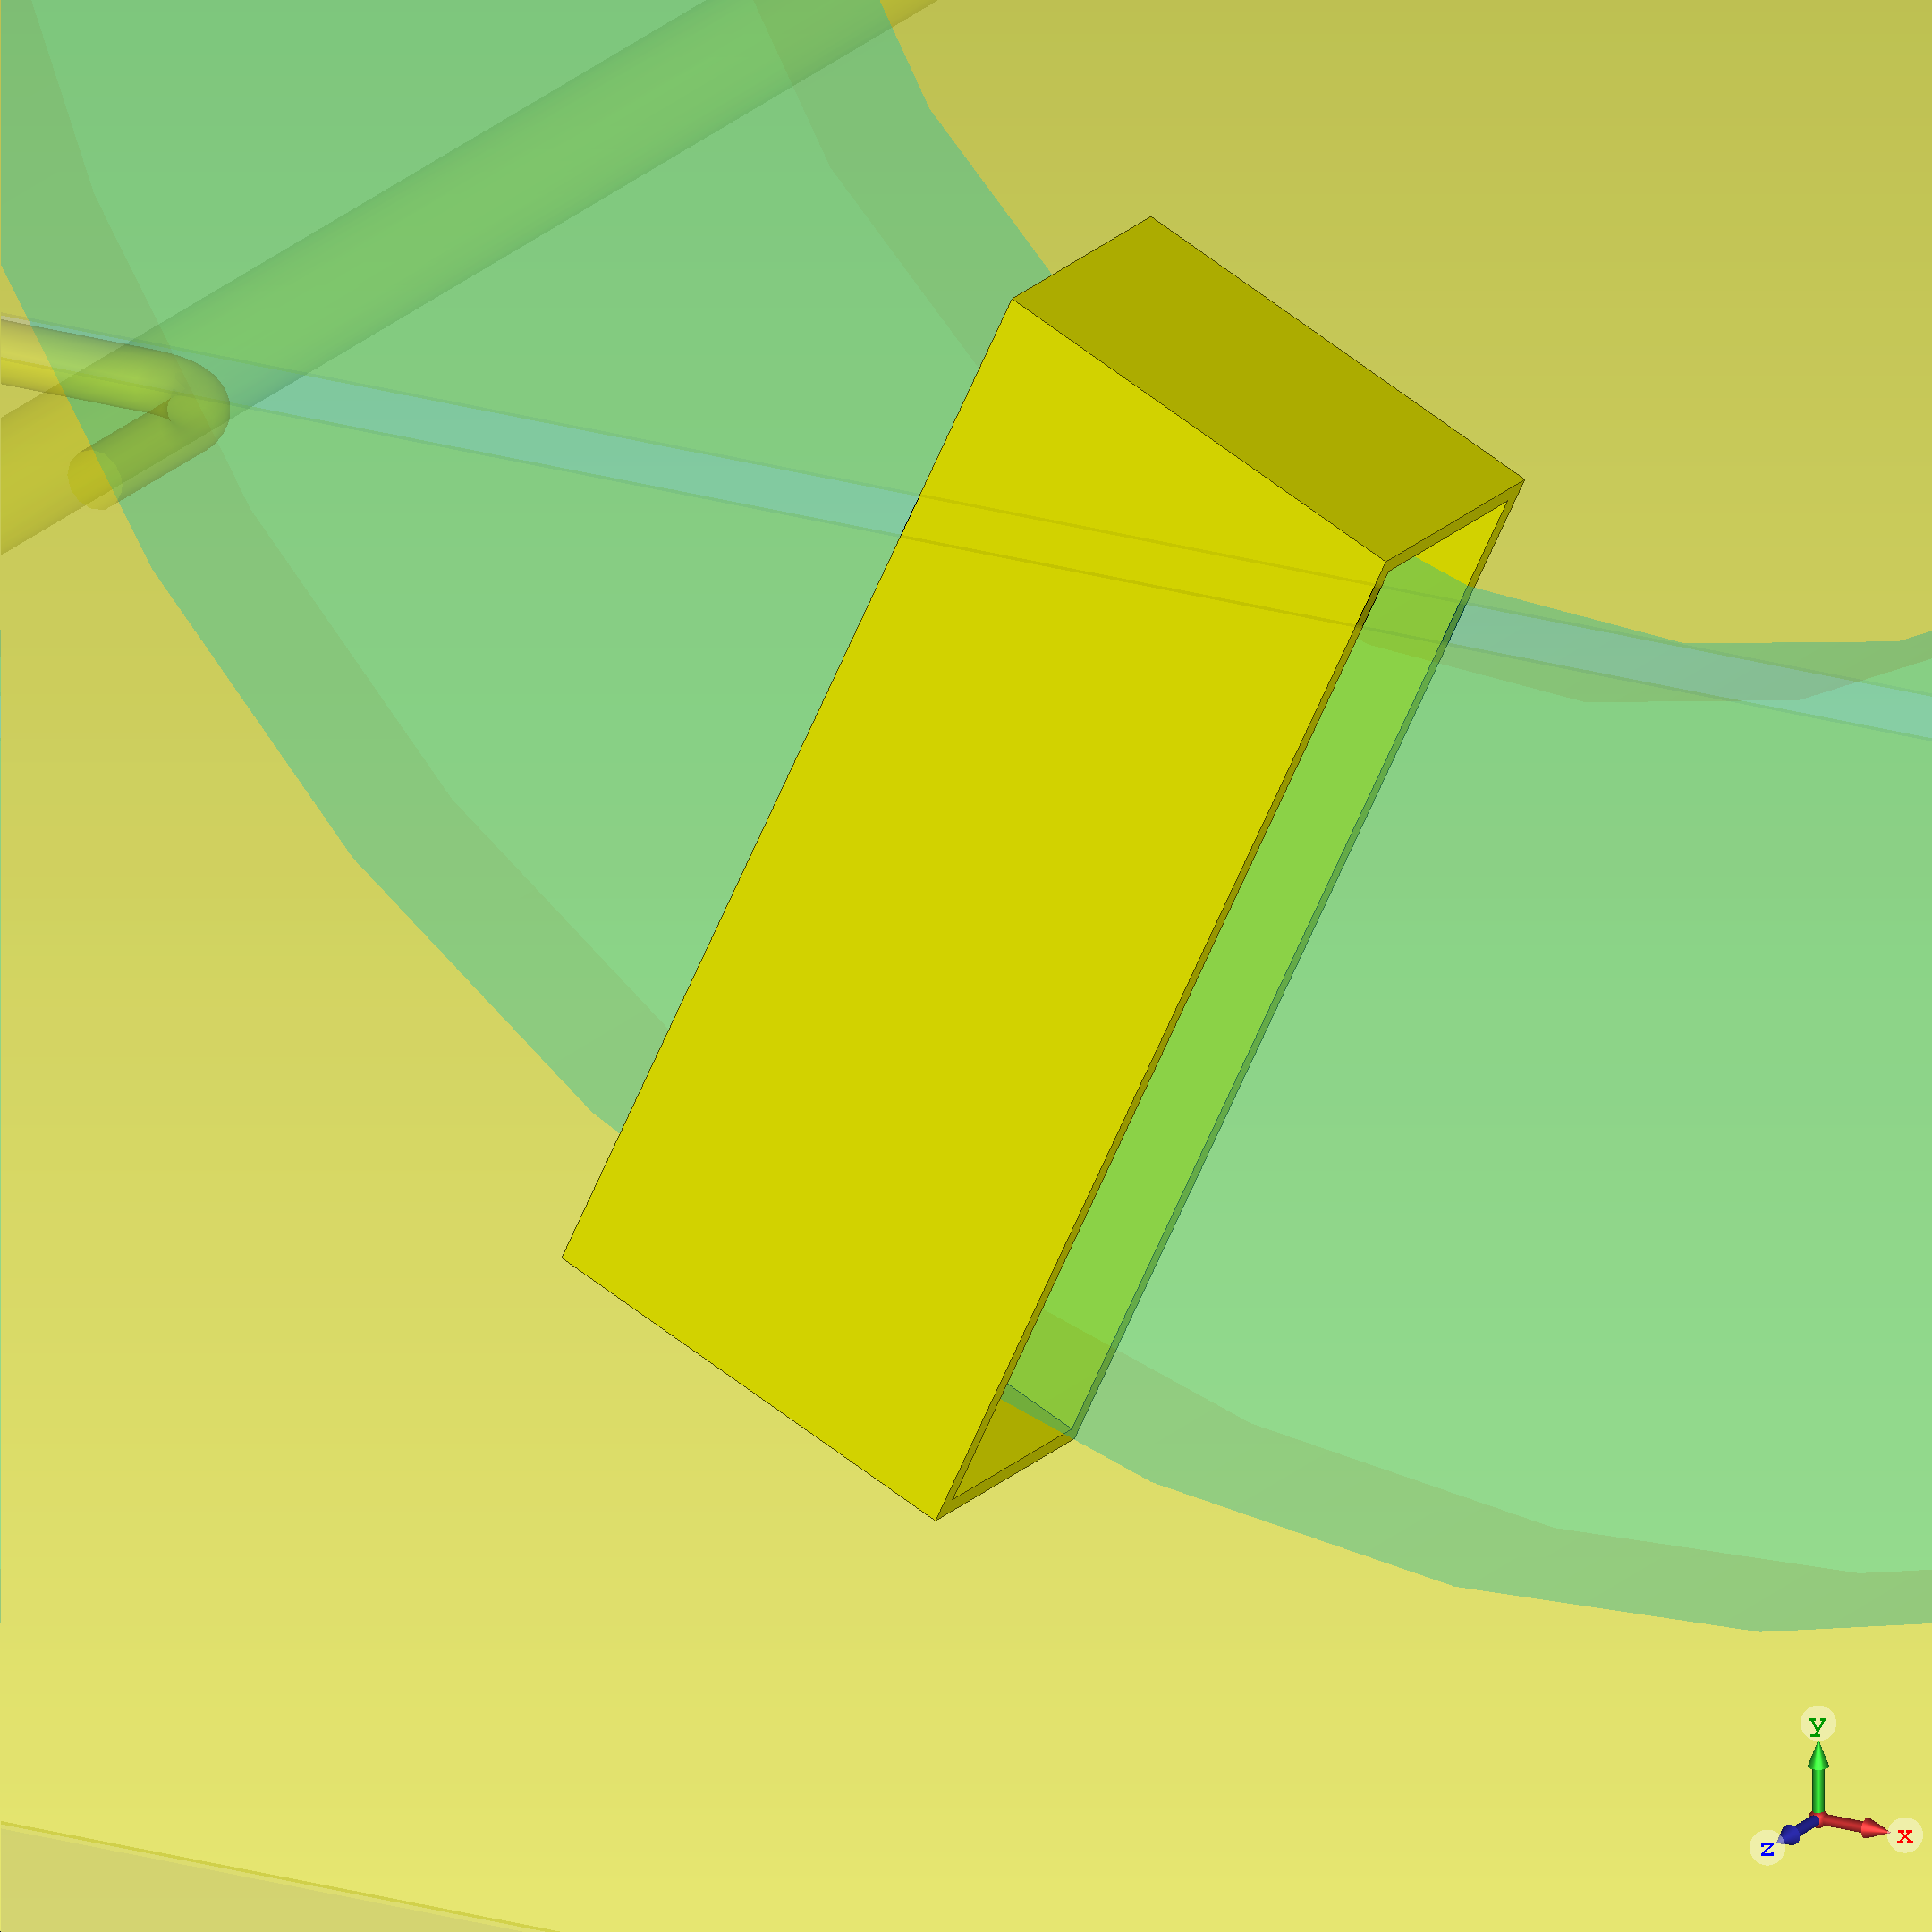
\includegraphics[height=0.3\textwidth]{./Simulation/KSV2Schiene.png}}
                \hspace{0.01\textwidth}
                \subfloat[Version 3]{
                    \label{subfig:V3}
                    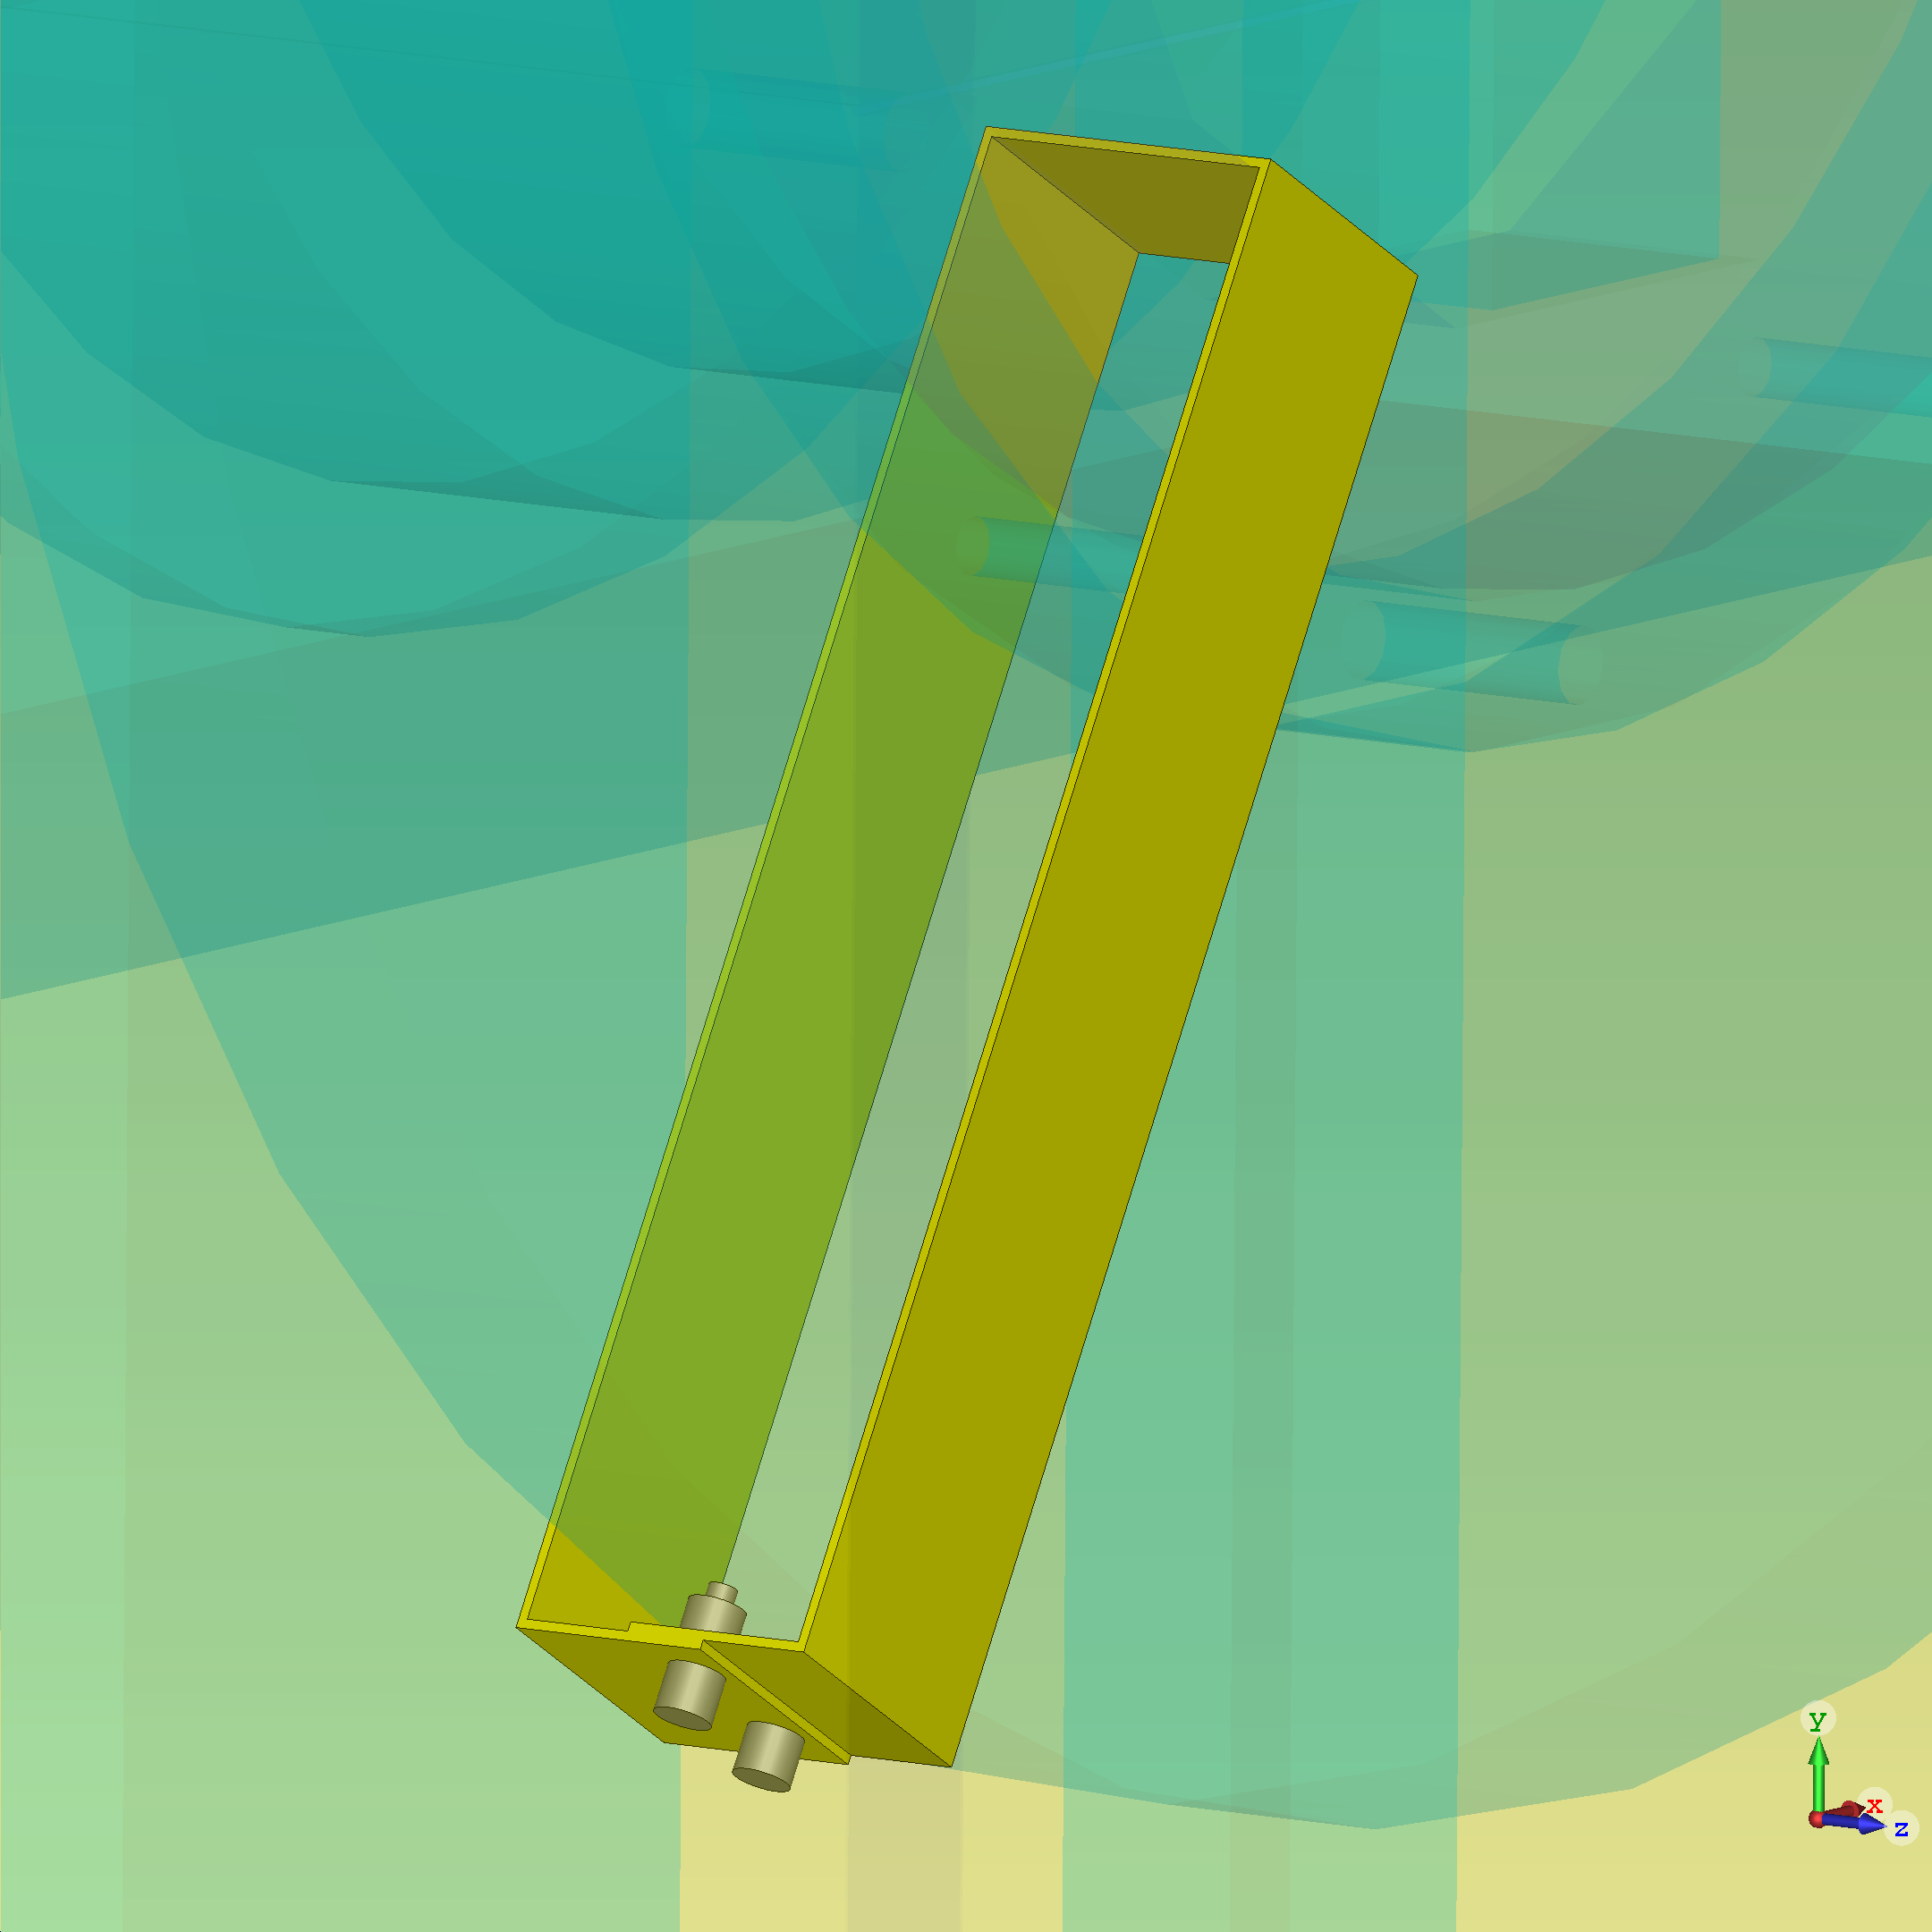
\includegraphics[height=0.3\textwidth]{./Simulation/KSV3MitSchrauben.png}}
                \caption{Modellierung eines Kurzschluss \protect\subref{subfig:V1} als Torus, \protect\subref{subfig:V2} als Schiene und \protect\subref{subfig:V3} in gefertigter Ausführung.}
                \label{fig:KSCST}
            \end{figure}
        
        Um eine Parameteranalyse durchzuführen und die Simulationsergebnisse mit den Messungen gegenüberzustellen, ist die finale Version in den verschiedenen Ausführungen, wie sie aus Kapitel~\ref{sec:shorts} hervorgehen, nachgebildet.
        
        \subsection{Realitätsgetreue Anpassungen}
        Das bestehende Modell wurde im Laufe der Arbeit weiter ausarbeitet, um die Übereinstimmung der Simulationsergebnisse mit den Messungen zu erhöhen. Die nachfolgenden Komponenten wurden in das CST-Modell übernommen, da aufgrund ihrer di-/elektrischen Eigenschaften ein Einfluss auf die Simulation zu erwarten ist.\\
        \todo[inline,color=red!30]{$\uparrow$ Verweis auf Simulationsergebnisse, wenn Kapitel vorhanden. $\uparrow$}
        Wie auf den Bildern der Testbox in Kapitel~\ref{chap:messaufbau} hervorgeht, befindet sich oberhalb der Einkopplungsstange an der Anschlussseite ein metallischer Bügel. Er ist möglichst exakt in CST nachgebildet (siehe Abb.~\ref{fig:AnpassungCST}\subref{subfig:Buegel}).\\
        Am Ende der Einkopplungsstange an der Rückwand ist eine zylinderförmige, kupferne Halterung für die Stange montiert, sie ist nach Abbildung~\ref{fig:AnpassungCST}\subref{subfig:Block} modelliert.
        \par
        Zuletzt wurde für diese Arbeit auch die Holzkonstruktion in CST übernommen, die als Halterung für die Ringkerne in der Testbox dient (siehe Abb.~\ref{fig:AnpassungCST}\subref{subfig:HolzKonst}). Dabei wurden die Holzkreise mit einem dissipativen, durch Austesten und die Messung Anpassen bestimmten $\underline{\varepsilon}_r(\omega) = \varepsilon_r'(\omega)-i\varepsilon_r''(\omega)$ modelliert, da es sich hierbei nicht um die Standardholzmodellierung von CST handelt, wie sie für die Holzbalken verwendet wird, sondern ein geschichtetes Pressspanholz verwendet wird.
        
            \begin{figure}[htb]
                \centering
                \subfloat[Bügel]{
                    \label{subfig:Buegel}
                    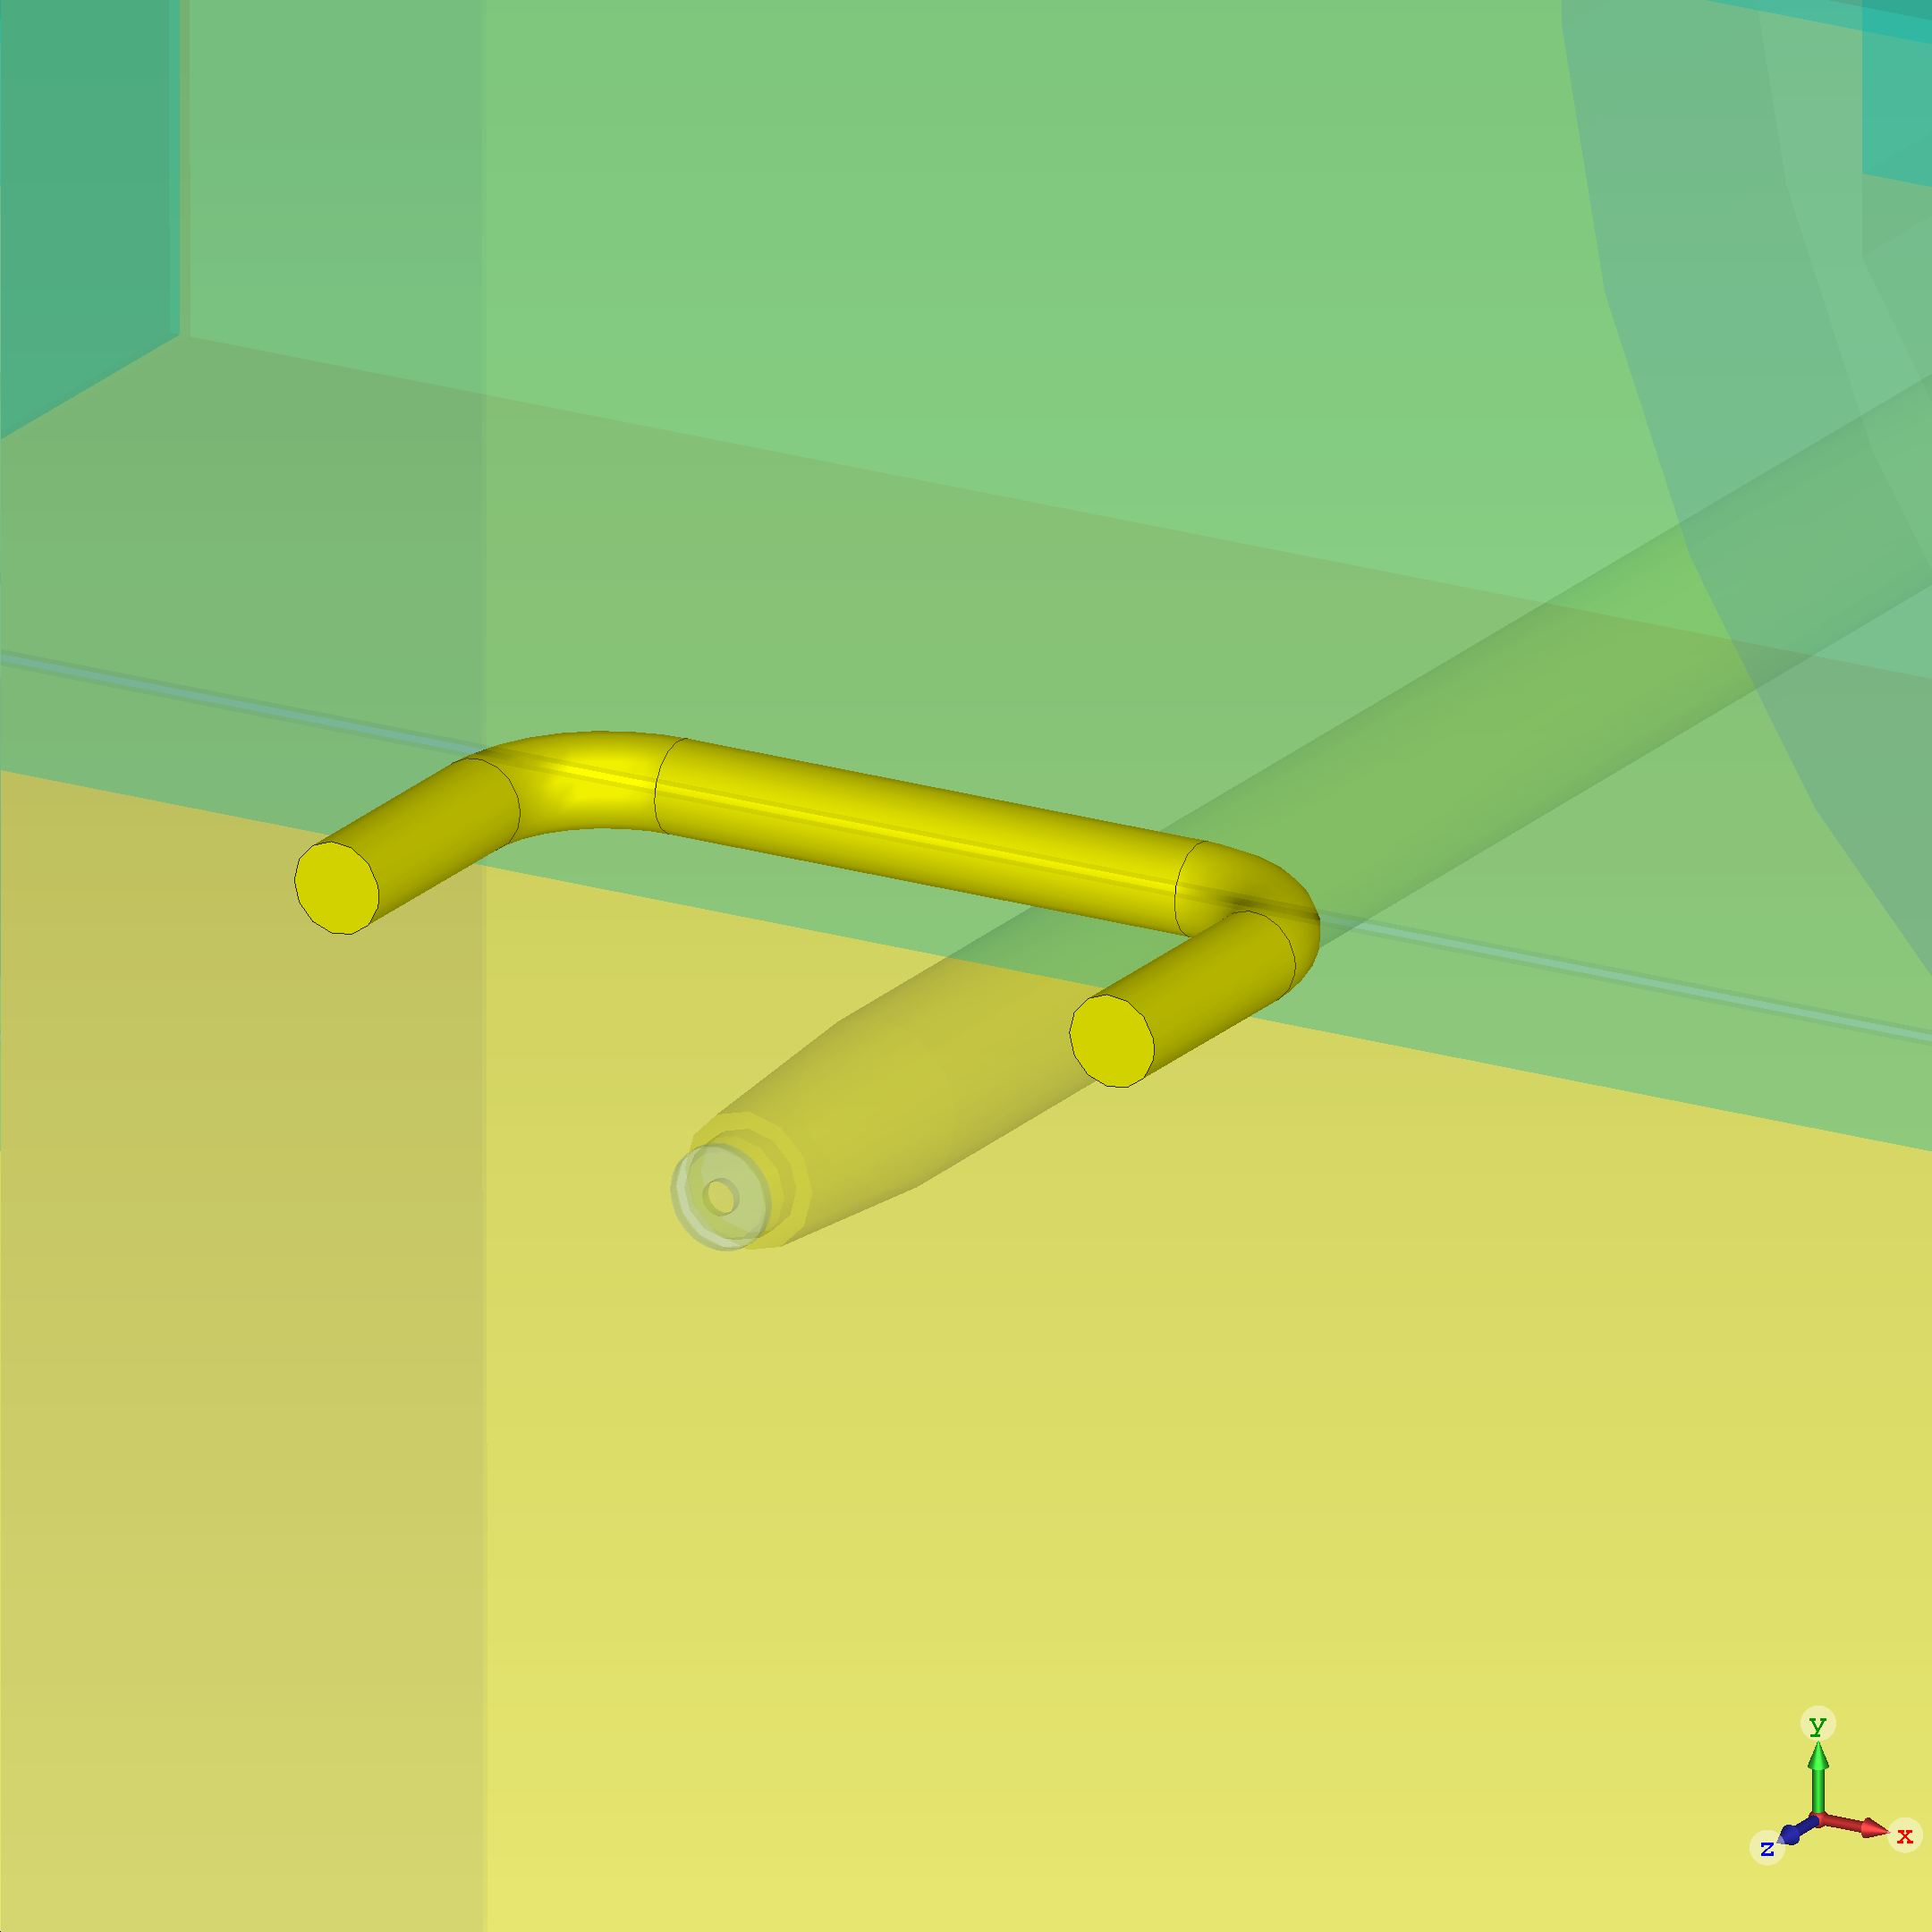
\includegraphics[height=0.3\textwidth]{./Simulation/Buegel.png}}
                \hspace{0.01\textwidth}
                \subfloat[Zylinder]{
                    \label{subfig:Block}
                    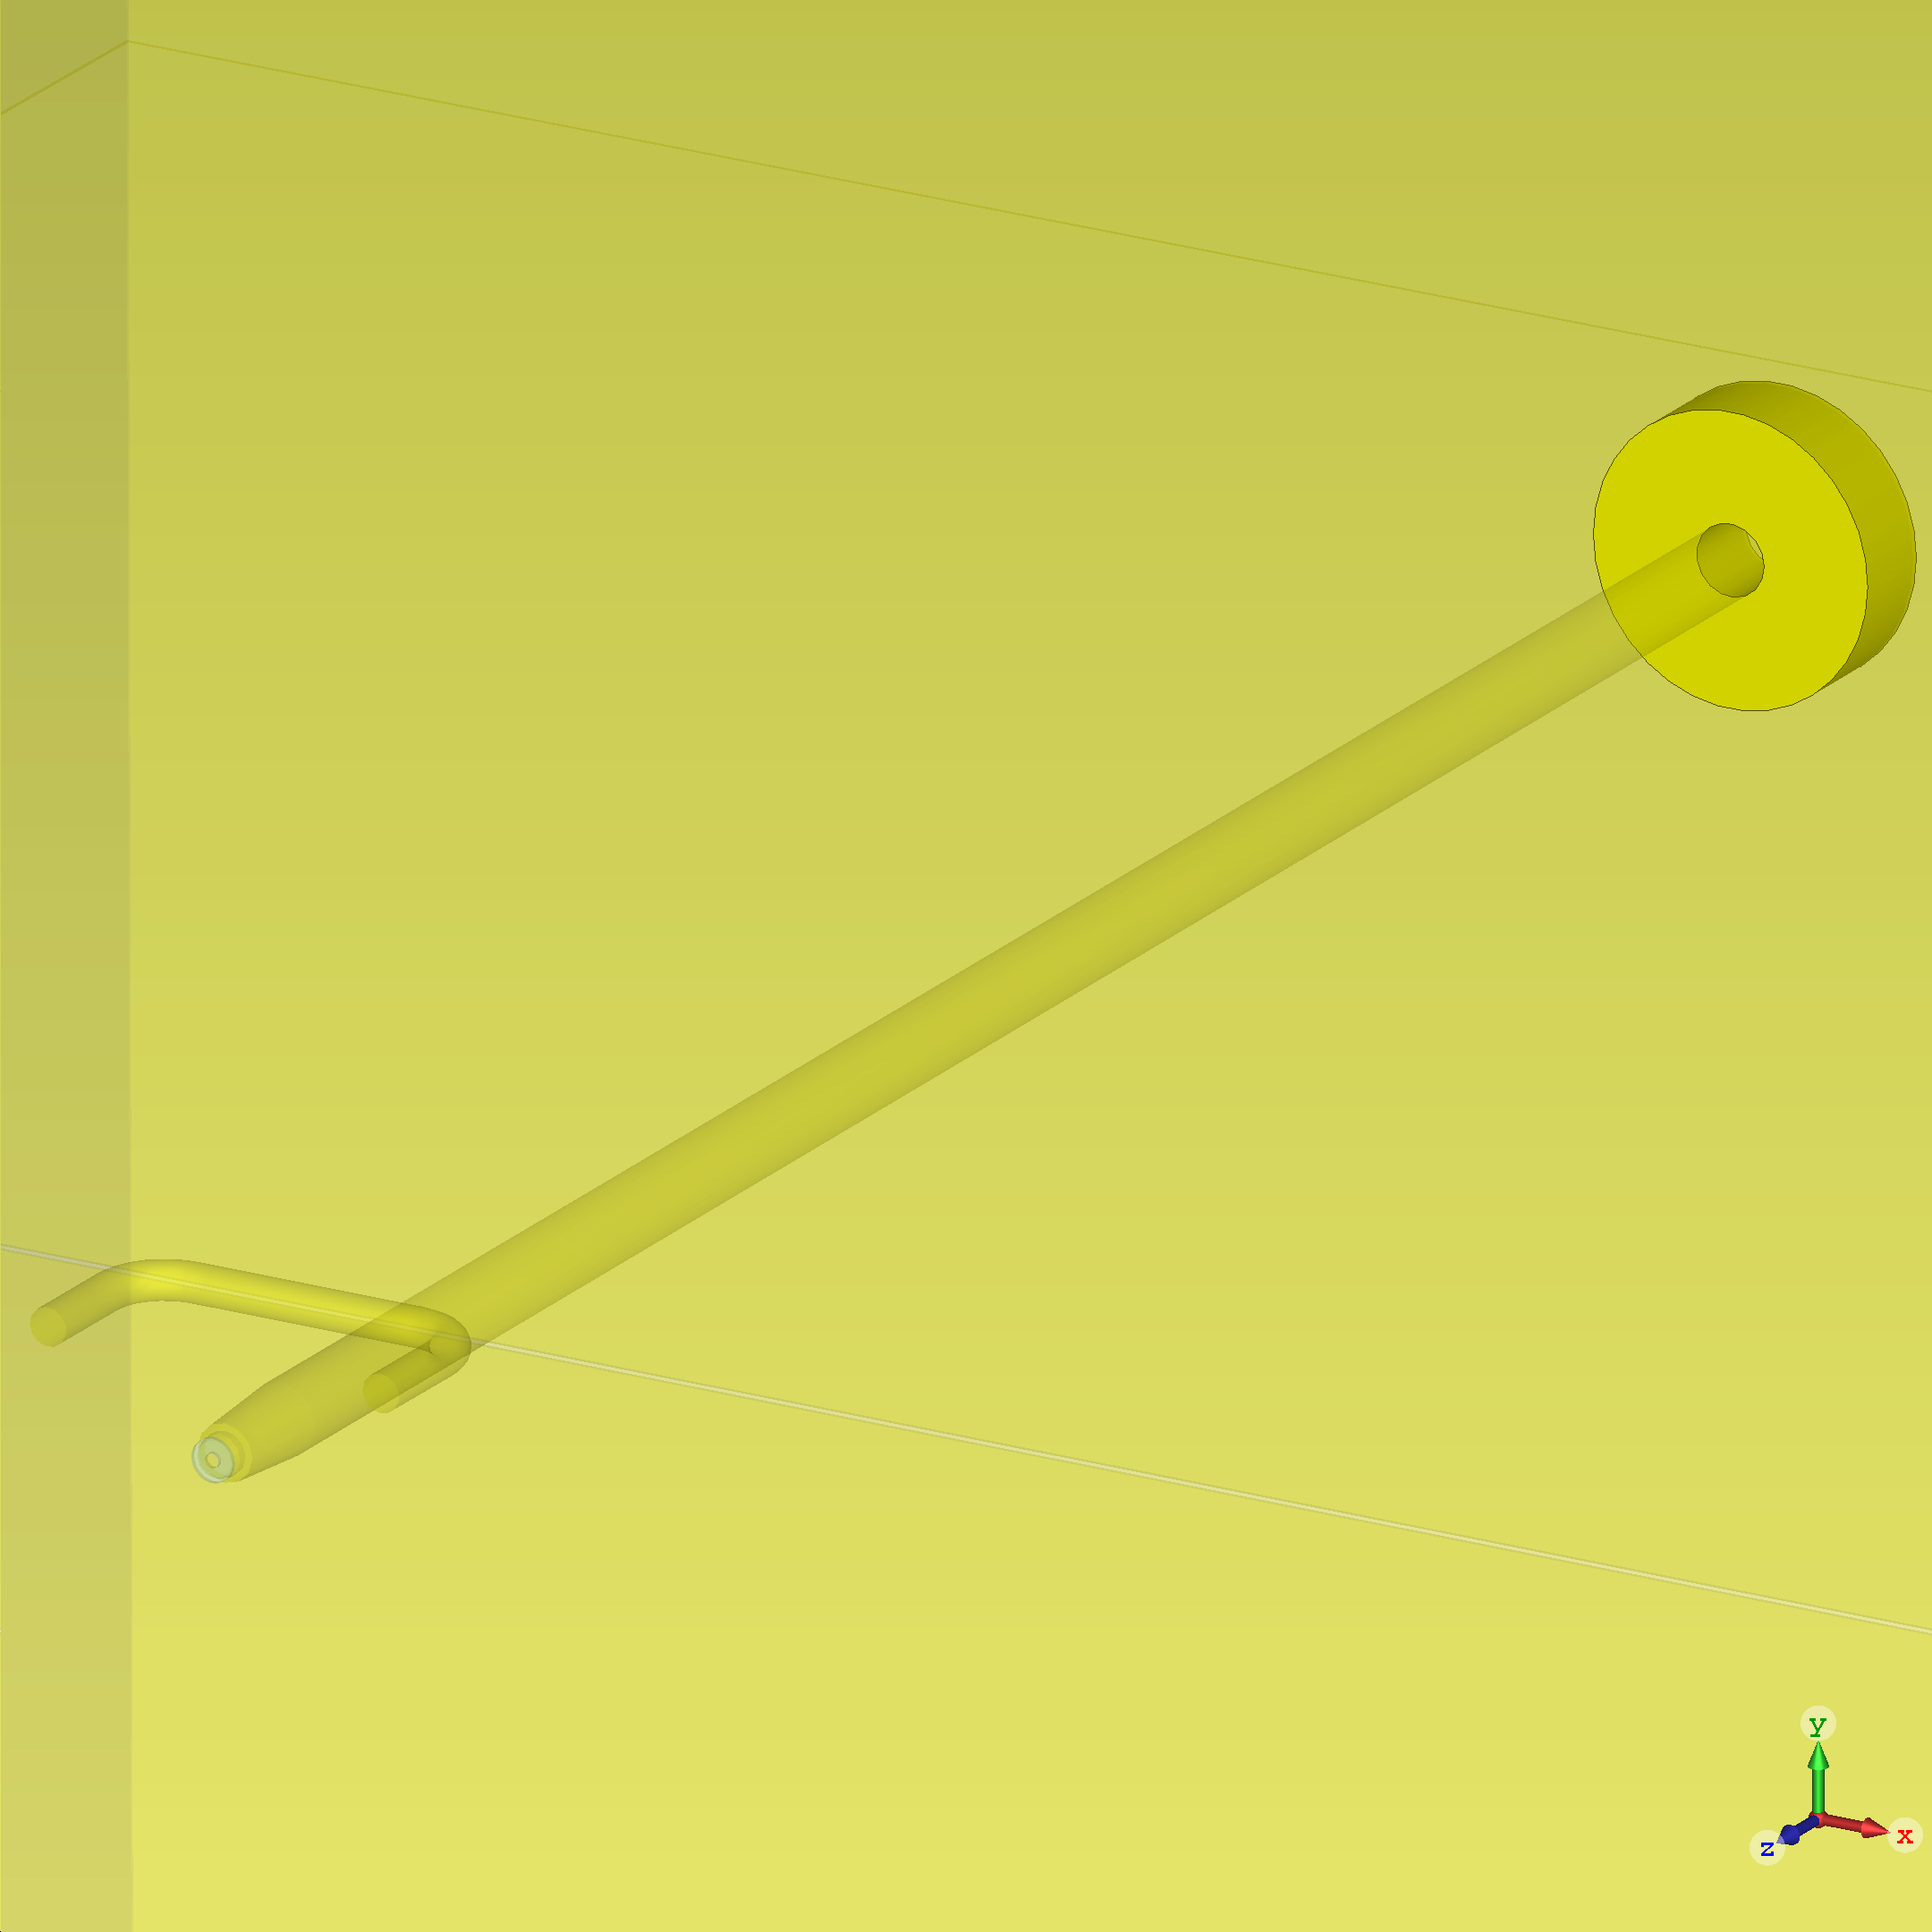
\includegraphics[height=0.3\textwidth]{./Simulation/Block.png}}
                \hspace{0.01\textwidth}
                \subfloat[Holzkonstruktion]{
                    \label{subfig:HolzKonst}
                    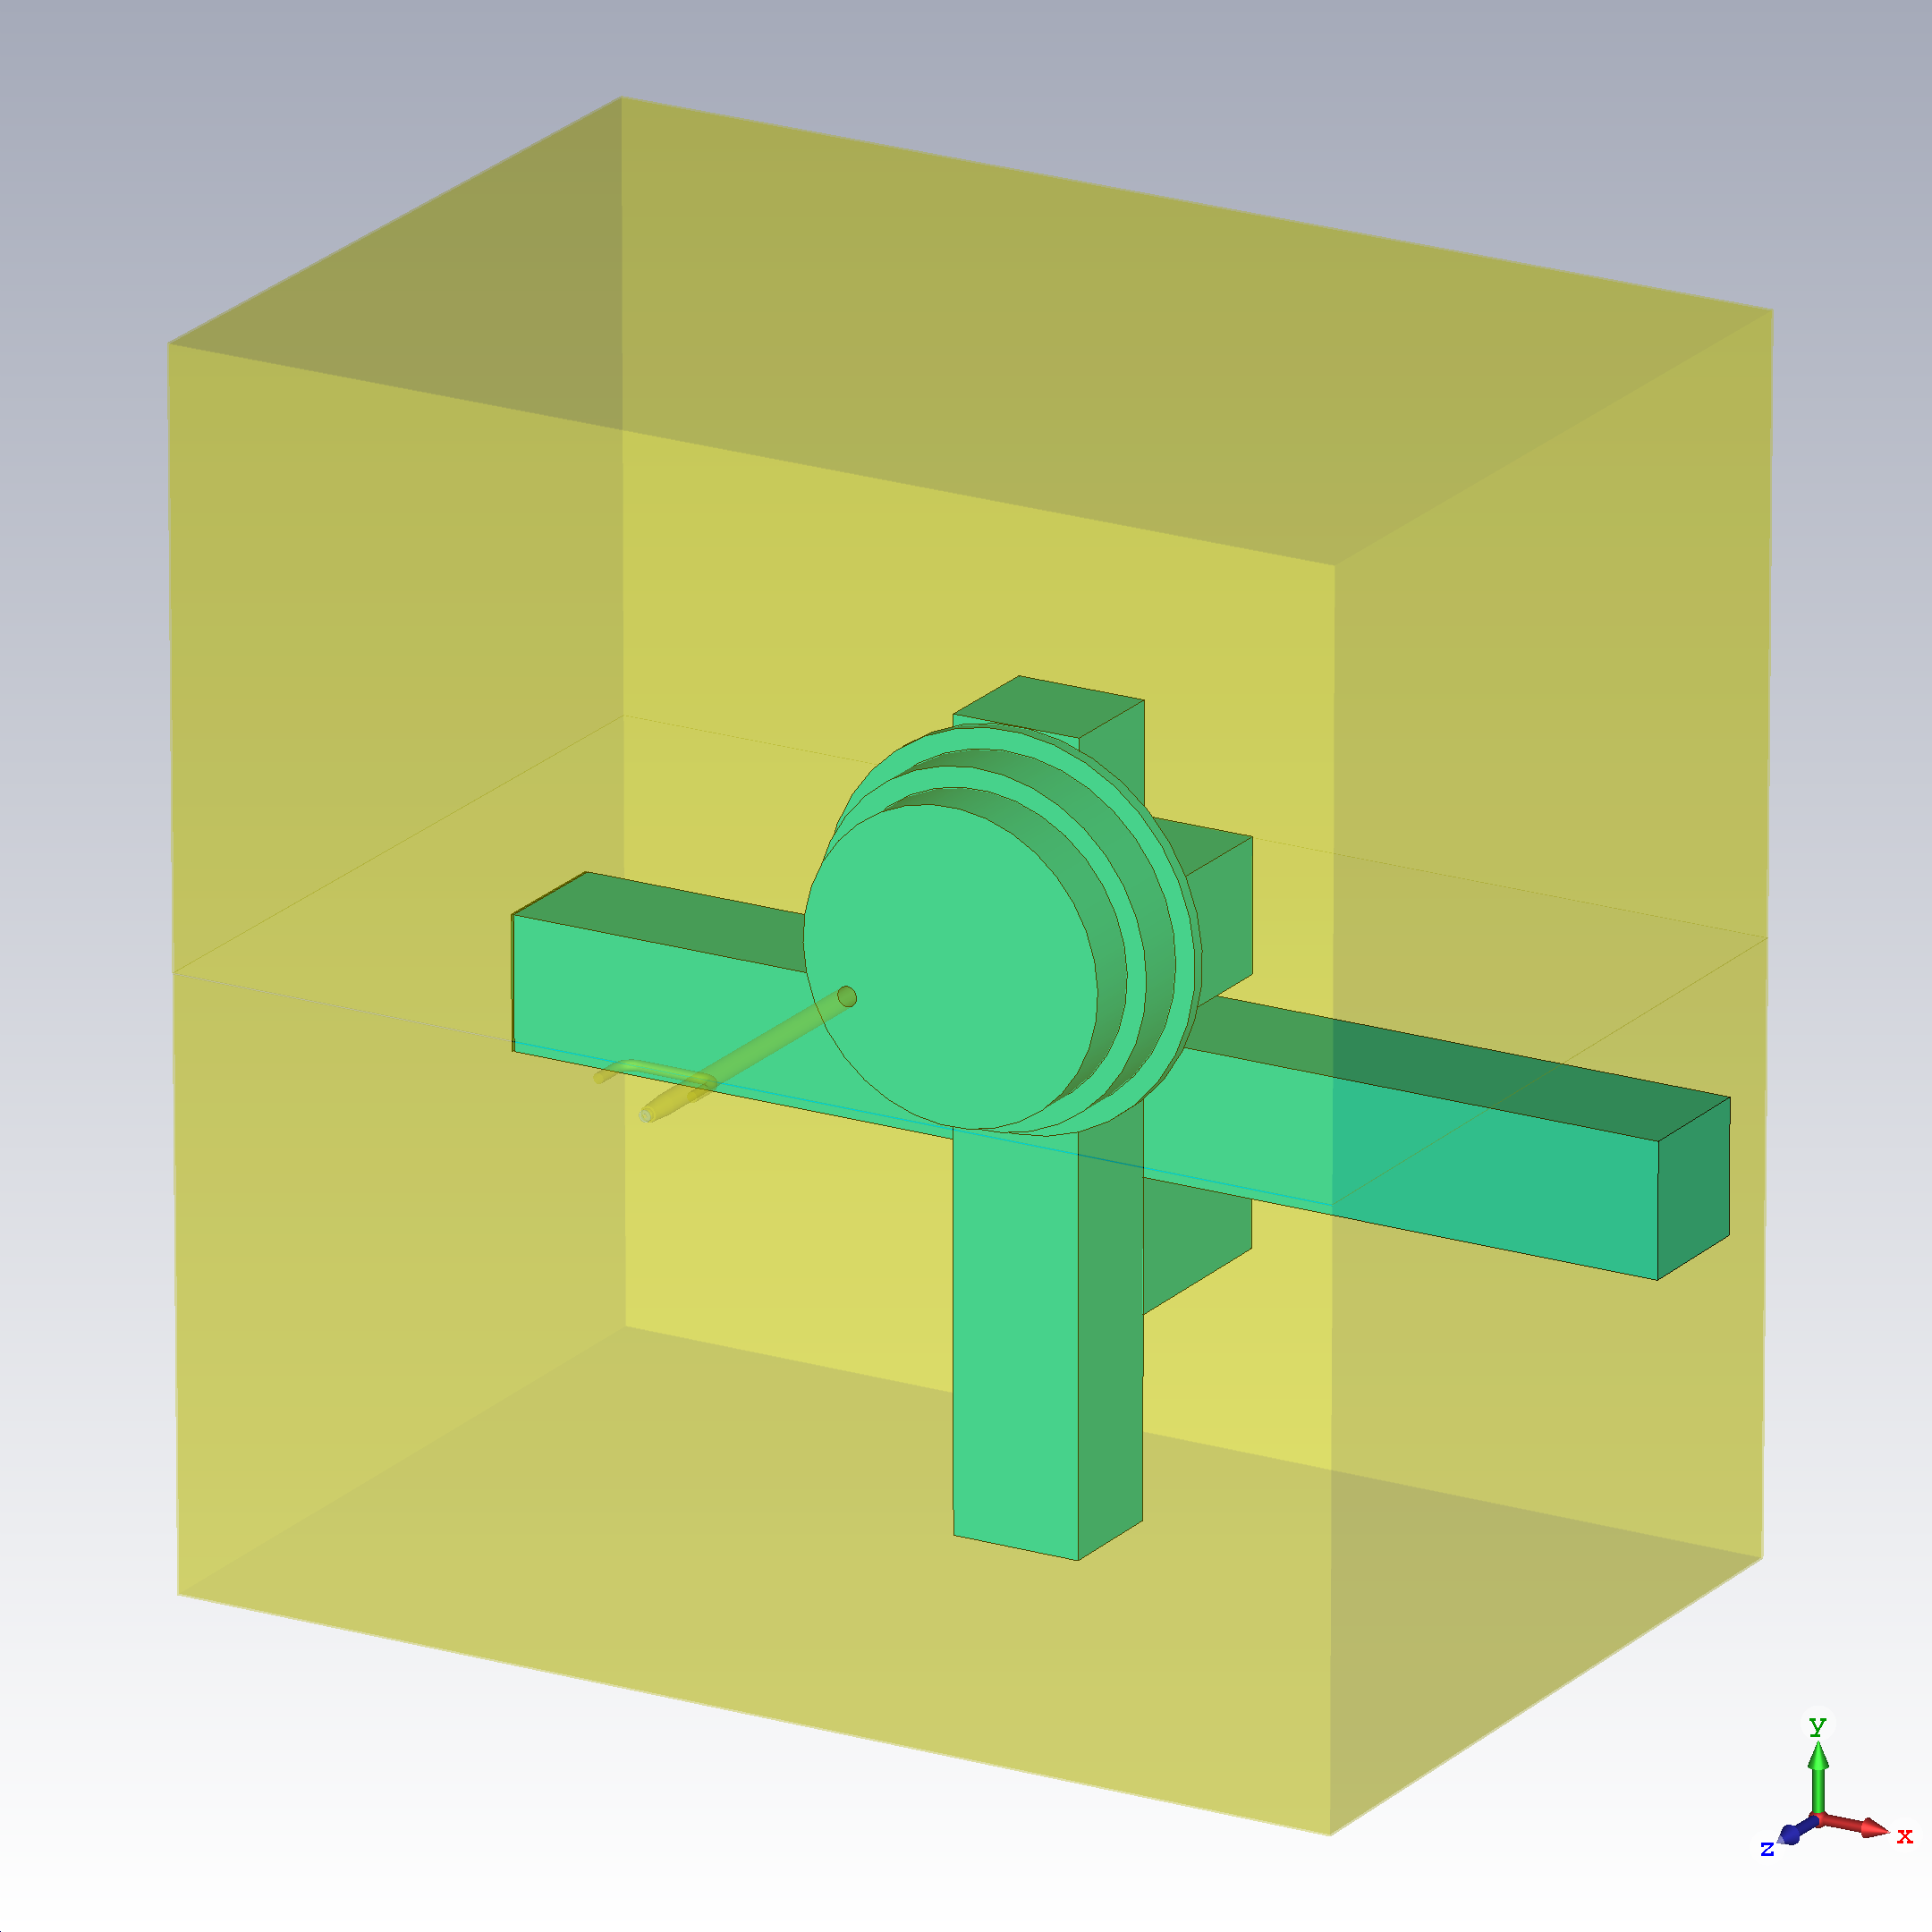
\includegraphics[height=0.3\textwidth]{./Simulation/HolzKonstrukt.png}}
                \caption{Anpassung des Simulationsmodells an den realen Aufbau \protect\subref{subfig:Buegel} Bügel über Einkopplung, \protect\subref{subfig:Block} Kupferzylinder an der Rückwand und \protect\subref{subfig:HolzKonst} die hölzerne Halterung des Ringkerns.}
                \label{fig:AnpassungCST}
            \end{figure}
        
            \subsubsection{Ringkern}
            \label{sec:ringkern}
            Die echten Ringkerne, wie sie bei der GSI benutzt werden, bestehen nicht nur aus dem MA-Material, sondern besitzen einen Innenkreis aus Eisen, der zur Montage dient. Da das Eisen andere magnetische Eigenschaften als das MA-Material besitzt, wurde dies in das Modell übernommen. Die neue Modellierung des Ringkerns mit innerem Eisenring ist in Abbildung~\ref{fig:RKFeRingCST} dargestellt.
                
                \begin{figure}[htb]
                    \centering
                    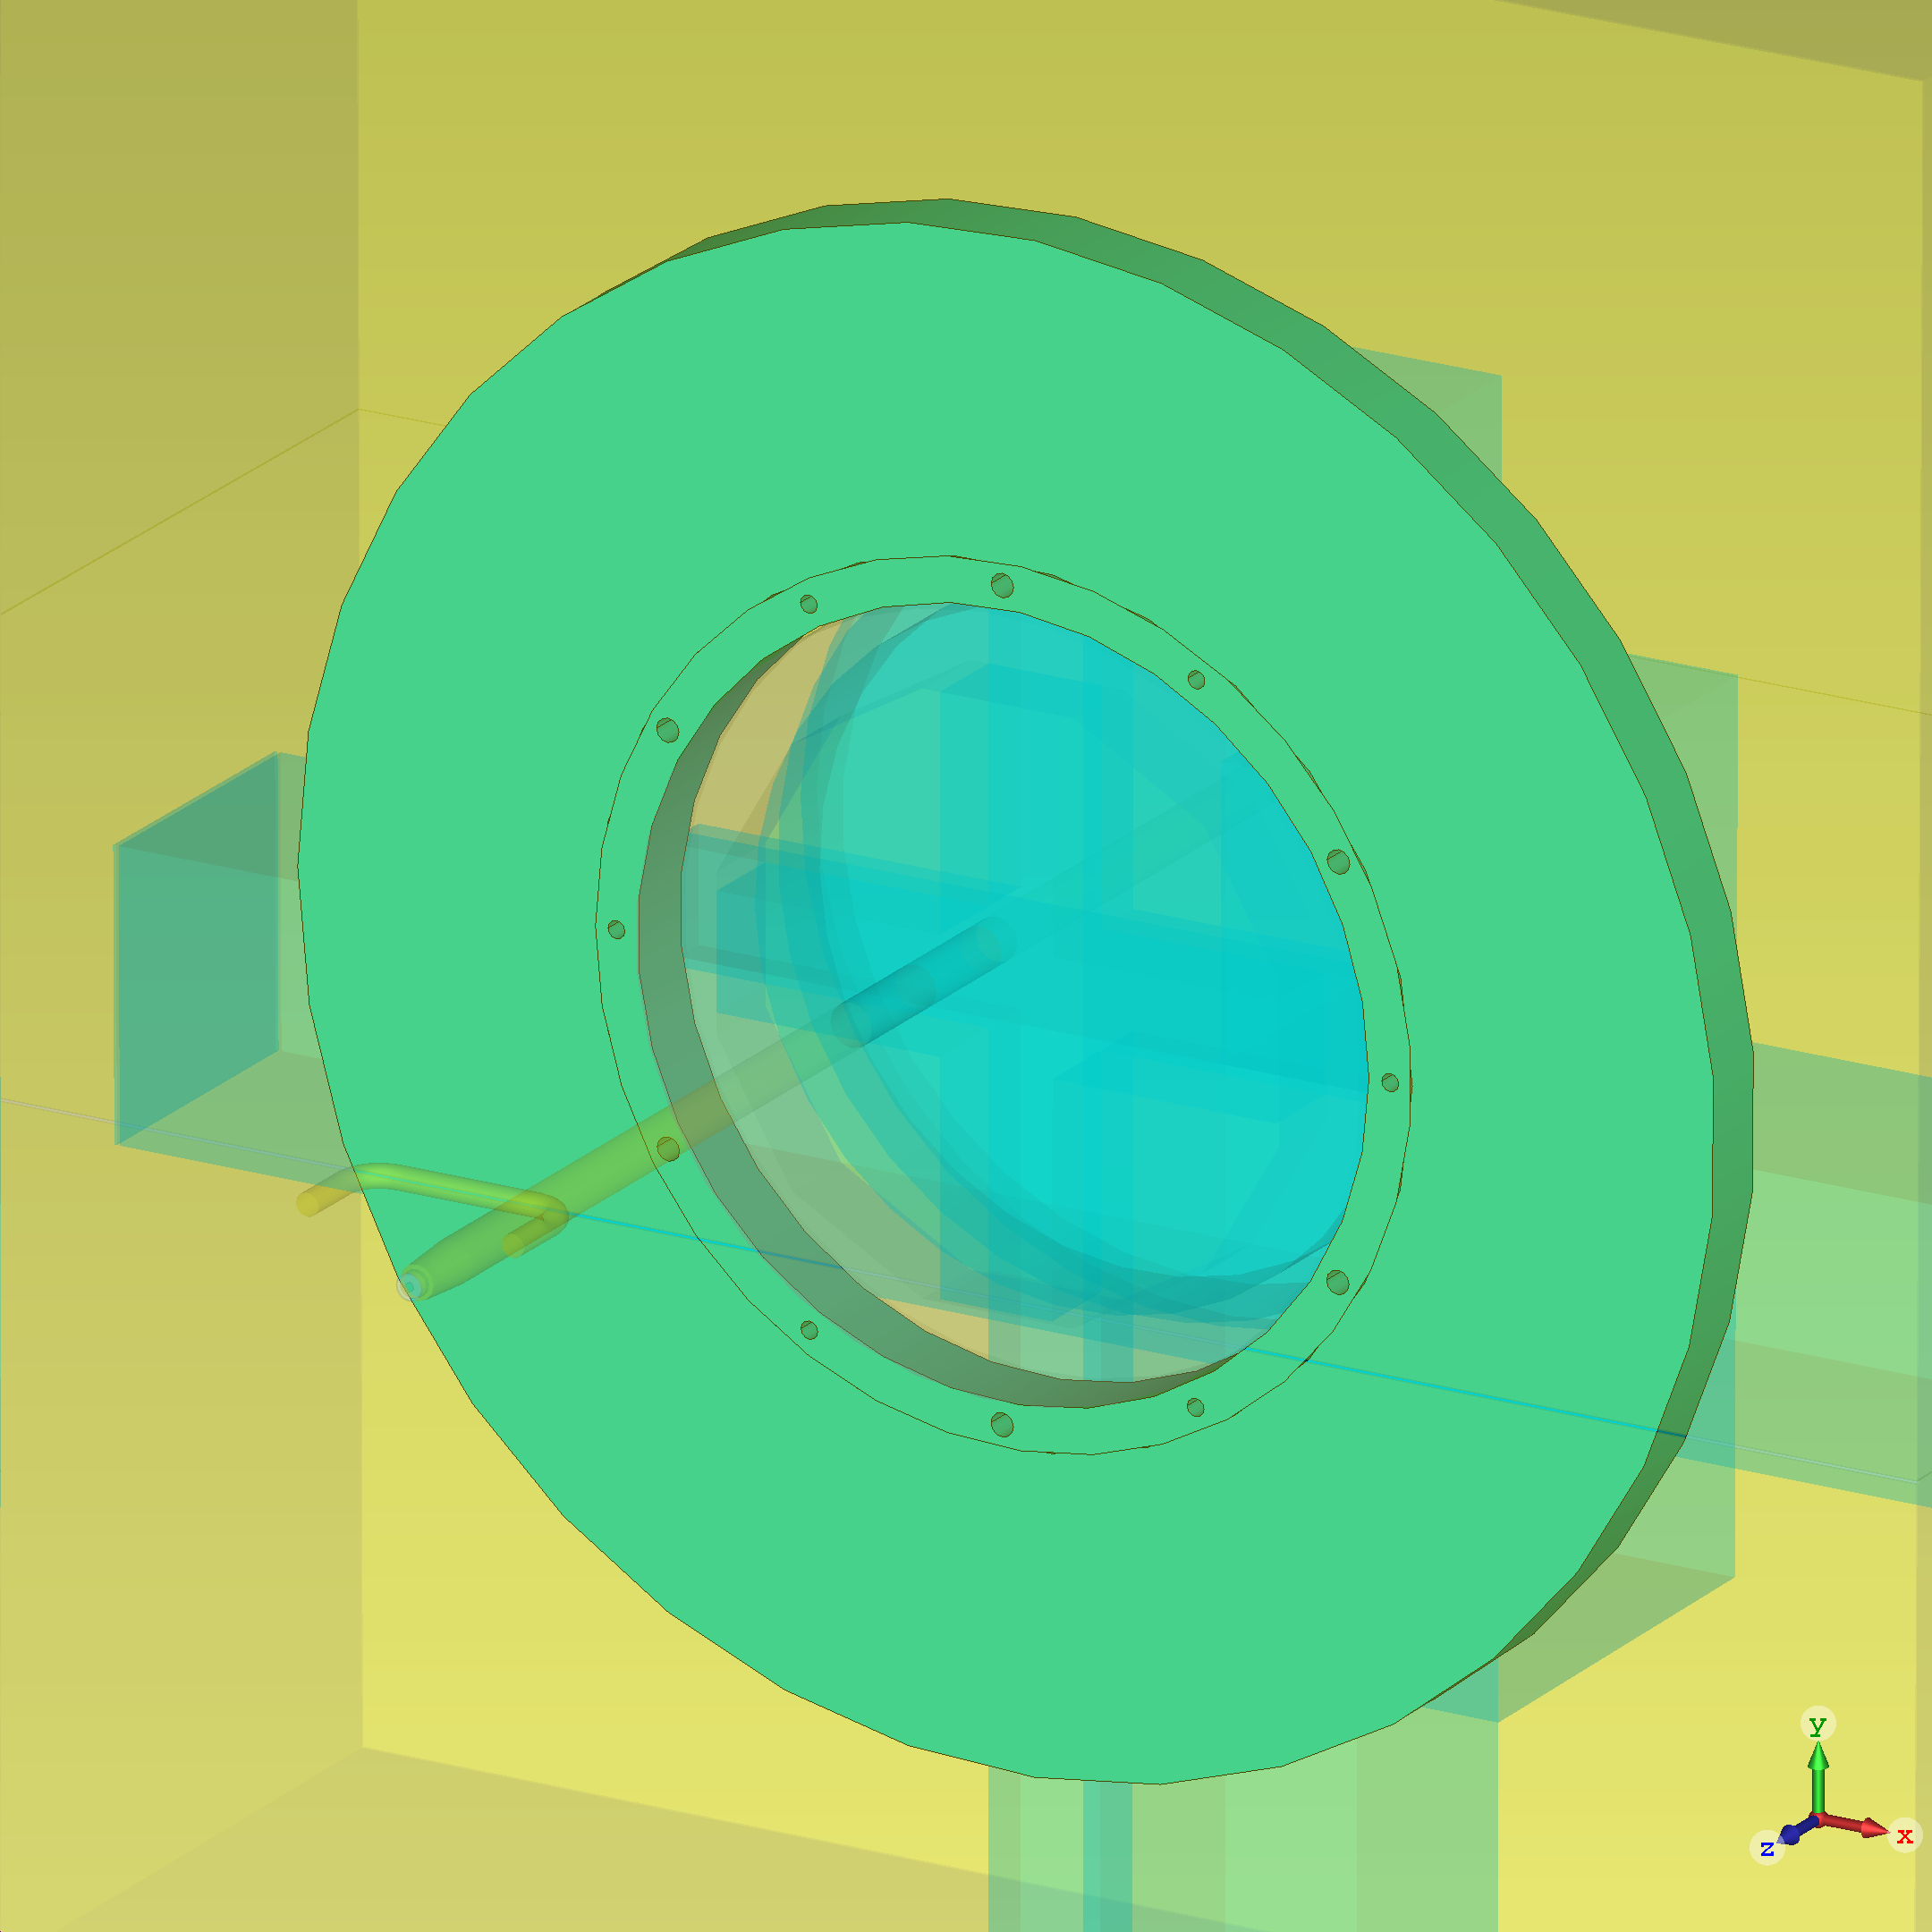
\includegraphics[height=0.4\textwidth]{./Simulation/RKFeRing.png}
                    \caption{Ringkernmodell mit innerem Eisenring}
                    \label{fig:RKFeRingCST}
                \end{figure}
            
            \par
            Des Weiteren wurde für eine bessere Übereinstimmung von Simulation und Messung die magnetische Permeabilität des Ringkernmaterials den Messungen entsprechend aktualisiert. Die Anpassung der Materialparameter basiert auf der Arbeit von Denys Bast~\citep{bast2017ba} und den theoretischen Grundlagen nach ~\citep{Klingbeil2008}.\\
            Die Testbox und der Ringkern können in ein Ersatzschaltbild überführt und damit der Impedanzverlauf analysiert werden. Das Ersatzschaltbild ist in Abbildung~\ref{fig:BoxRKCircuit} dargestellt, dabei wurde die Vorlage aus \citep{bast2017ba} um einen Widerstand ergänzt, der die Verluste der Anordnung nachbildet und für eine Dämpfung der Impedanzamplitude in Resonanz verantwortlich ist. Damit soll das hochfrequente Verhalten der Ersatzschaltung und der Messung besser in Übereinstimmung gebracht werden.\\
            Die Werte für die elektrischen Komponenten der Ersatzschaltung betragen:
                \begin{align}
                    R_{box} &= 16,46~k\Omega \nonumber\\
                    C_{box} &= 6,55~pF \nonumber\\
                    L_{box} &= 528,55~nH \nonumber
                \end{align}
            Die Impedanz dieser Anordnung bestimmt sich nach
                \begin{equation}\label{eq:Zges}
                    \underline{Z}_{ges} = \frac{R_{box}\cdot(\underline{Z}_{rk}+j\omega L_{box})}{R_{box}+(\underline{Z}_{rk}+j\omega L_{box})\cdot(1+j\omega R_{box}C_{box})}.
                \end{equation}
            Daraus lässt sich nun die Impedanz des Ringkerns $Z_{rk}$ bestimmen
                \begin{equation}\label{eq:Zrk}
                \underline{Z}_{rk} = \frac{\underline{Z}_{ges}\cdot(R_{box}+j\omega L_{box}-\omega^2\cdot R_{box}L_{box}C_{box}) - j\omega R_{box}L_{box}}{R_{box}-\underline{Z}_{ges}\cdot(1+j\omega R_{box}C_{box})}.
                \end{equation}
            Wird für $\underline{Z}_{ges}$ die Impedanz aus der Messung eingesetzt, kann die Ringkernimpedanz dieser Messung bestimmt werden.\\
            Nach~\citep{Klingbeil2008} kann diese als Reihenschaltung eines Widerstands $R_{rk}$ und einer Induktivität $L_{rk}$ als $\underline{Z}_{rk} = R_{rk}+j\omega L_{rk}$ betrachtet werden. Für das dissipative $\underline{\mu}_r = \mu' -j\mu''$  des Ringkerns wird in \citep{bast2017ba} angeführt, wie sich mittels der Ersatzschaltung $\mu'$ und $\mu''$ berechnen lassen:
                \begin{equation}
                    \mu' = \frac{L_{rk}\cdot 2\pi}{d\cdot ln\frac{r_a}{r_i}}
                \end{equation} 
                \begin{equation}
                \mu'' = \frac{R_{rk}\cdot\mu'}{\omega\cdot L_{rk}} .
                \end{equation}
            
                \begin{figure}[htb]
                    \centering
                    \begin{tikzpicture}
                    \node[above] at (-0.25,1.6) {$Z_{ges}$};
                    \draw (-0.5,1.4) -- (0.1,1.4);
                    \draw (-0.5,1.6) -- (0.1,1.6);
                    \path[fill=black, draw=black]
                        (0.1,1.3)  -- (0.1,1.7)  -- (0.5,1.5) --  (0.1,1.3);
                    \begin{circuitikz}
                    \draw
                    (2,0) to [resistor =$R_{box}$] (2,3)
                    (5,0) to [C, l=$C_{box}$] (5,3)
                    (5,3) to [L, l=$L_{box}$] (9,3)
                    (9,3) to [short, *-] (10,3)
                    (9,0) to [short, *-] (10,0)
                    (10,3) to [resistor =$Z_{rk}$] (10,0)
                    (0,3) to [short, *-] (5,3)
                    (0,0) to [short, *-] (5,0)
                    (8,3) to [short, -*] (9,3)
                    (5,0) to [short, -*] (9,0);
                    % 		(0,0) to [short, *- , i_=$I_5$] (1.5,-2);
                    \end{circuitikz}
                    \end{tikzpicture}
                    \caption{RLC-Ersatzschaltbild f\"ur die Testbox Modellierung mit Eingebrachtem Ringkern als Last.}
                    \label{fig:BoxRKCircuit}
                \end{figure}
                
            Ausgehend vom angepassten, dissipativen $\underline{\mu}_r$ kann nun die Simulation aktualisiert werden. Dazu werden die bestimmten Werte für $\mu'$ und $\mu''$ als Materialparameter in CST hinterlegt.
           
        \subsection{Erweiterung des Modells}
        Wie bereits in Kapitel~\ref{chap:messaufbau} erläutert, wurde die Testbox für die einfachere Montage der Kurzschlüsse und die erhöhte Reproduzierbarkeit der Messungen modifiziert und um ein kreuzförmiges Gestell aus Holz, sowie einen nichtleitenden Ring mit einem Polygonzug als Innenkreis erweitert (Geometrie und Beschreibung siehe Kapitel~\ref{chap:messaufbau}). Diese Modifikationen sind mit CST geometrisch genau nachgebildet (siehe Abb.~\ref{fig:KreuzPolygonCST}). Für das Holzkreuz wurden die selben Materialparameter verwendet, die für die Holzkreise hinterlegt sind, da es sich auch hierbei das Pressspanholz handelt.
        
            \begin{figure}[htb]
                \centering
                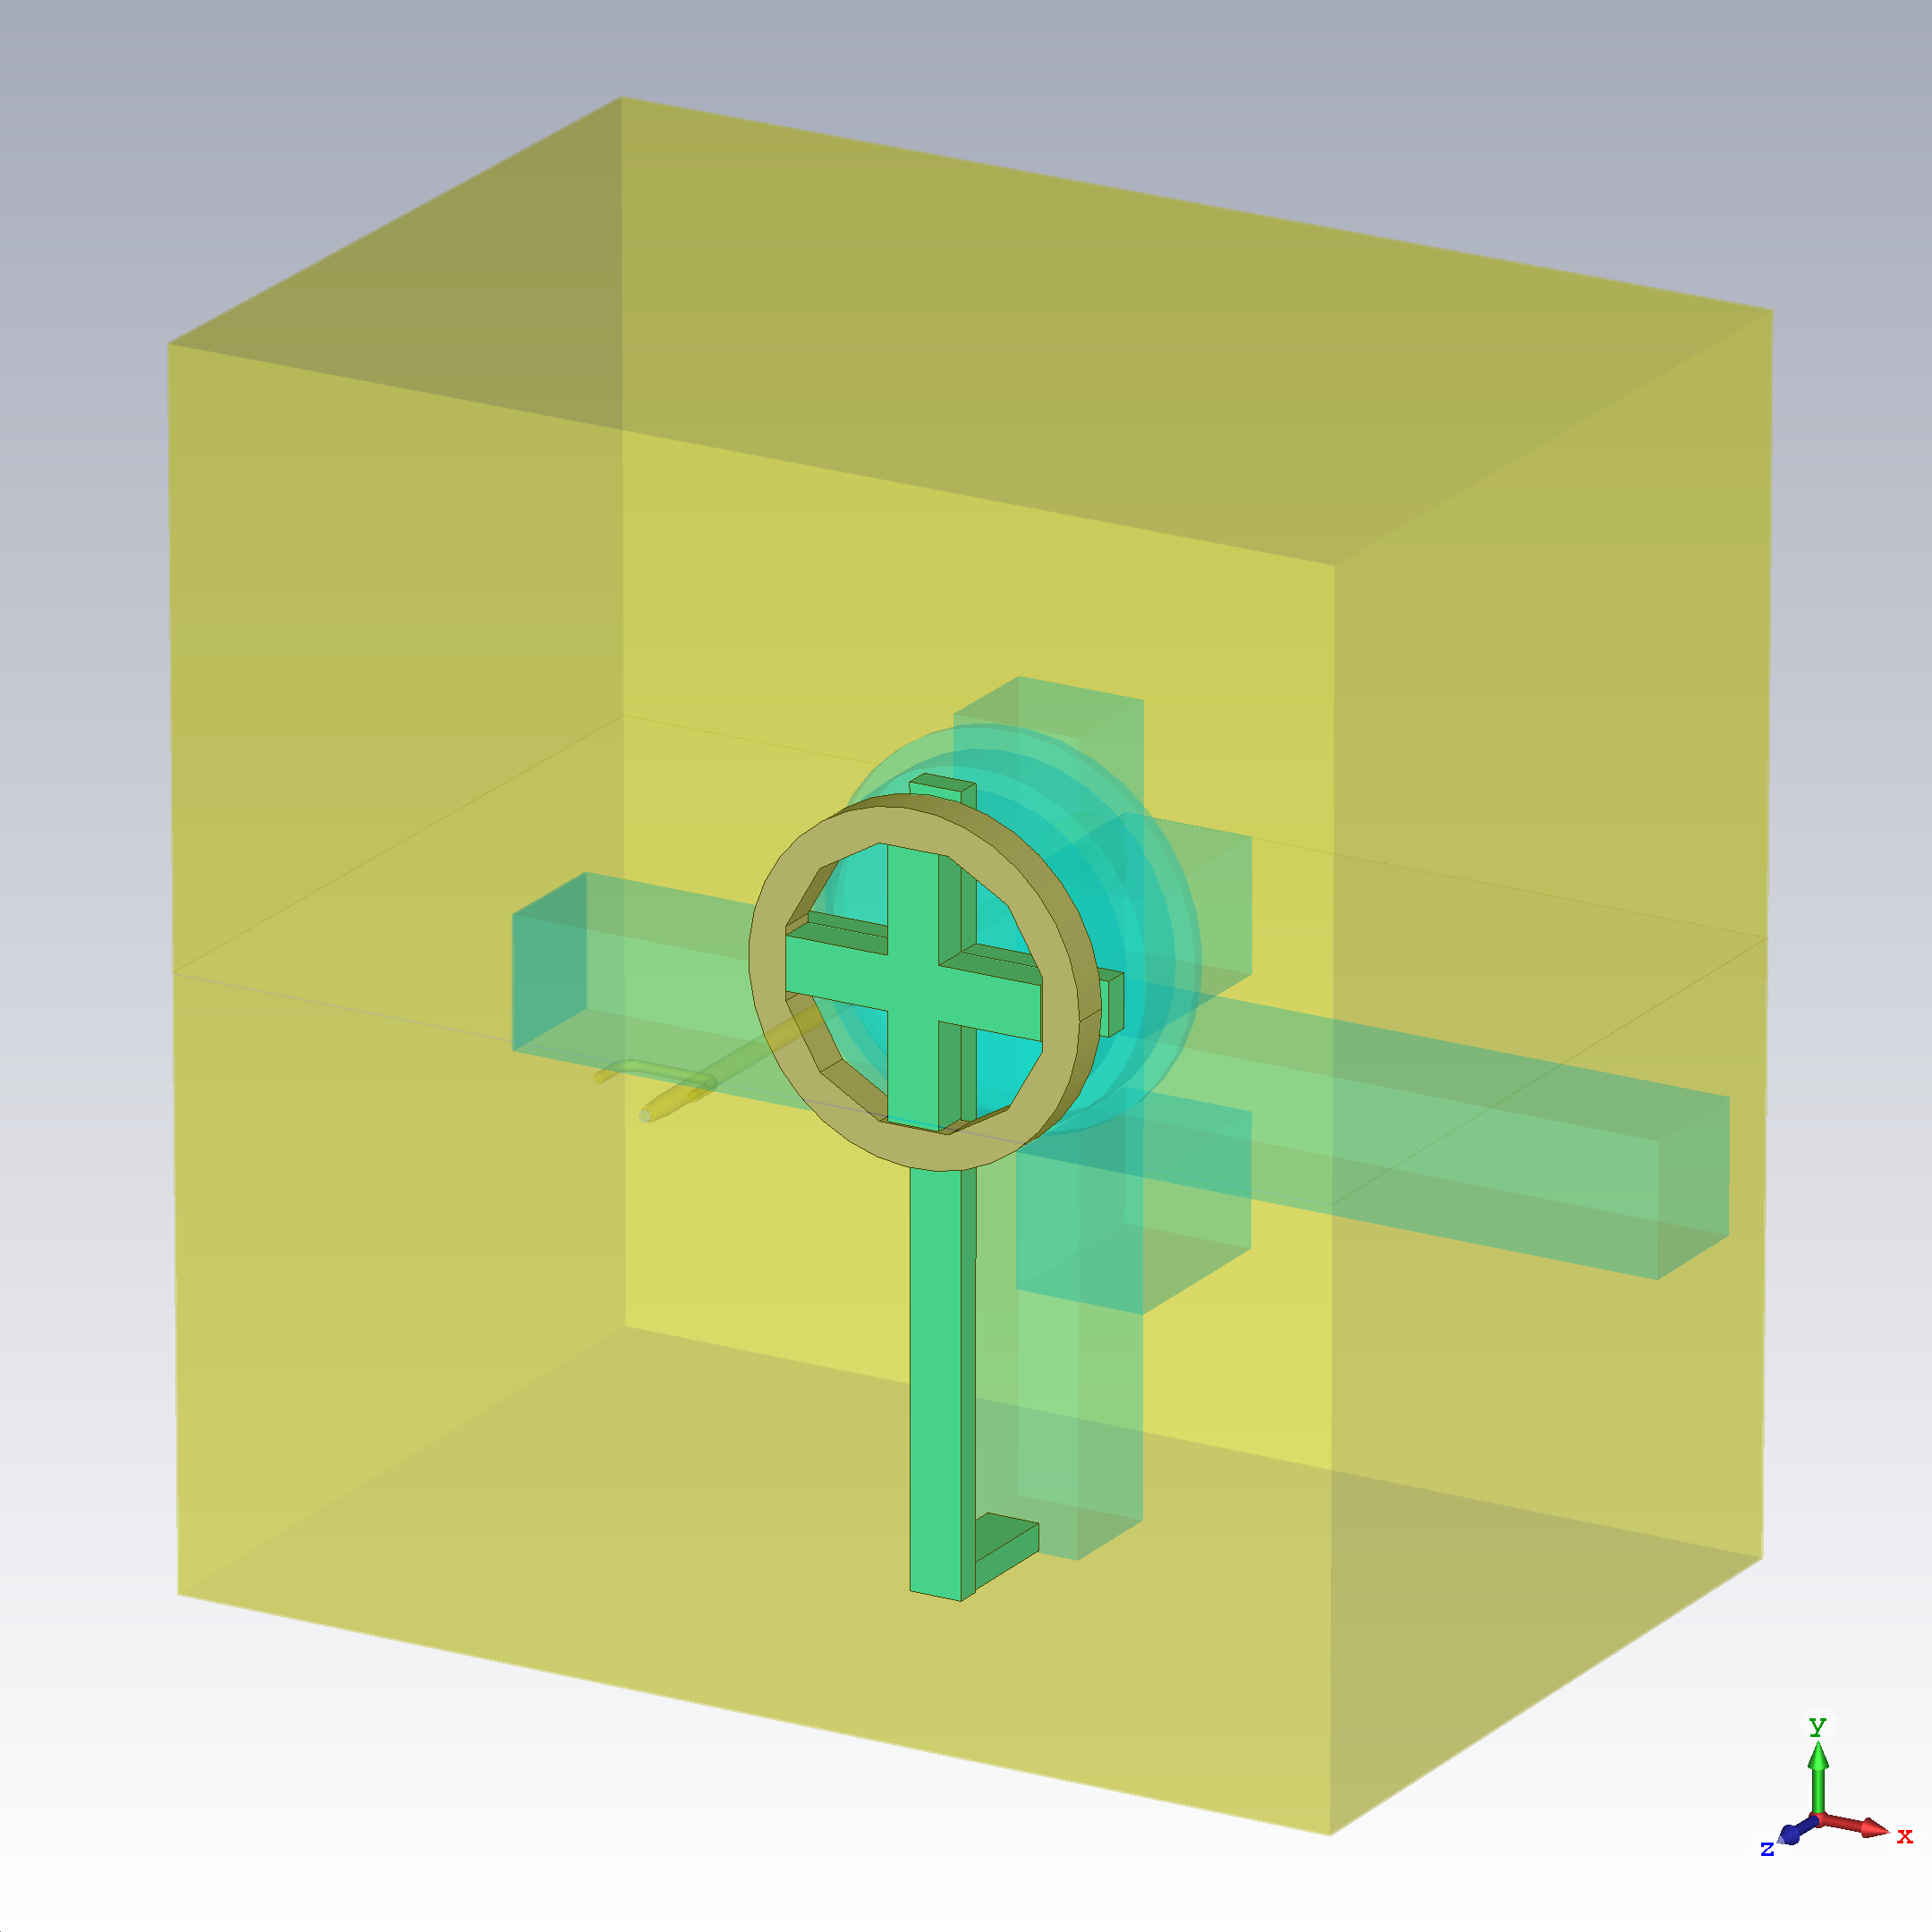
\includegraphics[height=0.4\textwidth]{./Simulation/KreuzPolygon.png}
                \caption{Erweiterung der Testbox um die Holzkreuzhalterung und den Polygonzug zur Befestigung der Kurzschlüsse}
                \label{fig:KreuzPolygonCST}
            \end{figure}
        
    \section{Durchführung}
    
    \todo[inline,color=red!30]{Hier weiter ausarbeiten!}
    
    \sout{Dieser Text soll nicht sein.}\textcolor{red}{Dieser Schon.}


%	\section{Testbox und Material}
Wie in Abschnitt~\ref{sec:testbox} angef\"uhrt, kann das Modell f\"ur die Simulationen in Grundz\"ugen aus der Bachelorarbeit von Denys Bast~\cite{bast2017ba} \"ubernommen werden. Die Modellierung der Testbox mitsamt Ringkern wurde dabei in mehreren Schritten durchgef\"uhrt. Die W\"ande der Testbox wurden mit idealem Kupfer modelliert. Ebenso wurde die Einkopplung und der Innenleiter durch die Box mit idealem Kupfer dargestellt und die Dimensionen der Verbindung entsprechend angepasst. Die Holzkonstruktion zur Halterung der Rinkerne ist im Urspr\"unglichen Modell nicht modelliert, der Ringkern h\"angt dort also in der Luft.
\par
Der Ringkern selbst, beziehungsweise das Ringkernmaterial wurde aus der Messung herausgezogen. Dazu wurde die Messkurve der Ringkernbox als RLC-Modellierung gefittet. Aus den berechneten Werte f\"ur L und C k\"onnen anschlie\ss{}end die Parameter $\mu'$ und $\mu''$ mit Hilfe der Formeln $1$ bis $3$ berechnet werden.

%	\section{Variation der Parameter}
	
\chapter{Gegen\"uberstellung und Ergebnisse}\label{chap:ergebnis}
	\section{Gegen\"uberstellung der Simulations und Messergebnisse}\label{sec:gegenueberst}
Ausgehend von den beschriebenen Modellierungsschritten kann nun eine sichere Evaluierung der Kurzschlussanordnungen angesetzt werden. Dabei k\"onnen die Messungen sowie das Simulationsmodell zur Kreuzvalidierung verwendet werden, sodass Mess- und Simulationsfehler weitestgehend auszuschlie\ss{}en sind. Dazu wurde das Simulationsmodell, nach den in Absatz~\ref{chap:simulation} versehenen Anpassungen zun\"achst einmal zur Referenz mit den Messungen verglichen. Dazu wird die Testbox ohne Ringkern, jedoch mit fertigem Halterungsaufbau gegen\"ubergestellt. Abbildung~\ref{fig:boxpolycross} zeigt diese Gegen\"uberstellung.

\begin{figure}[htb]
	\centering
	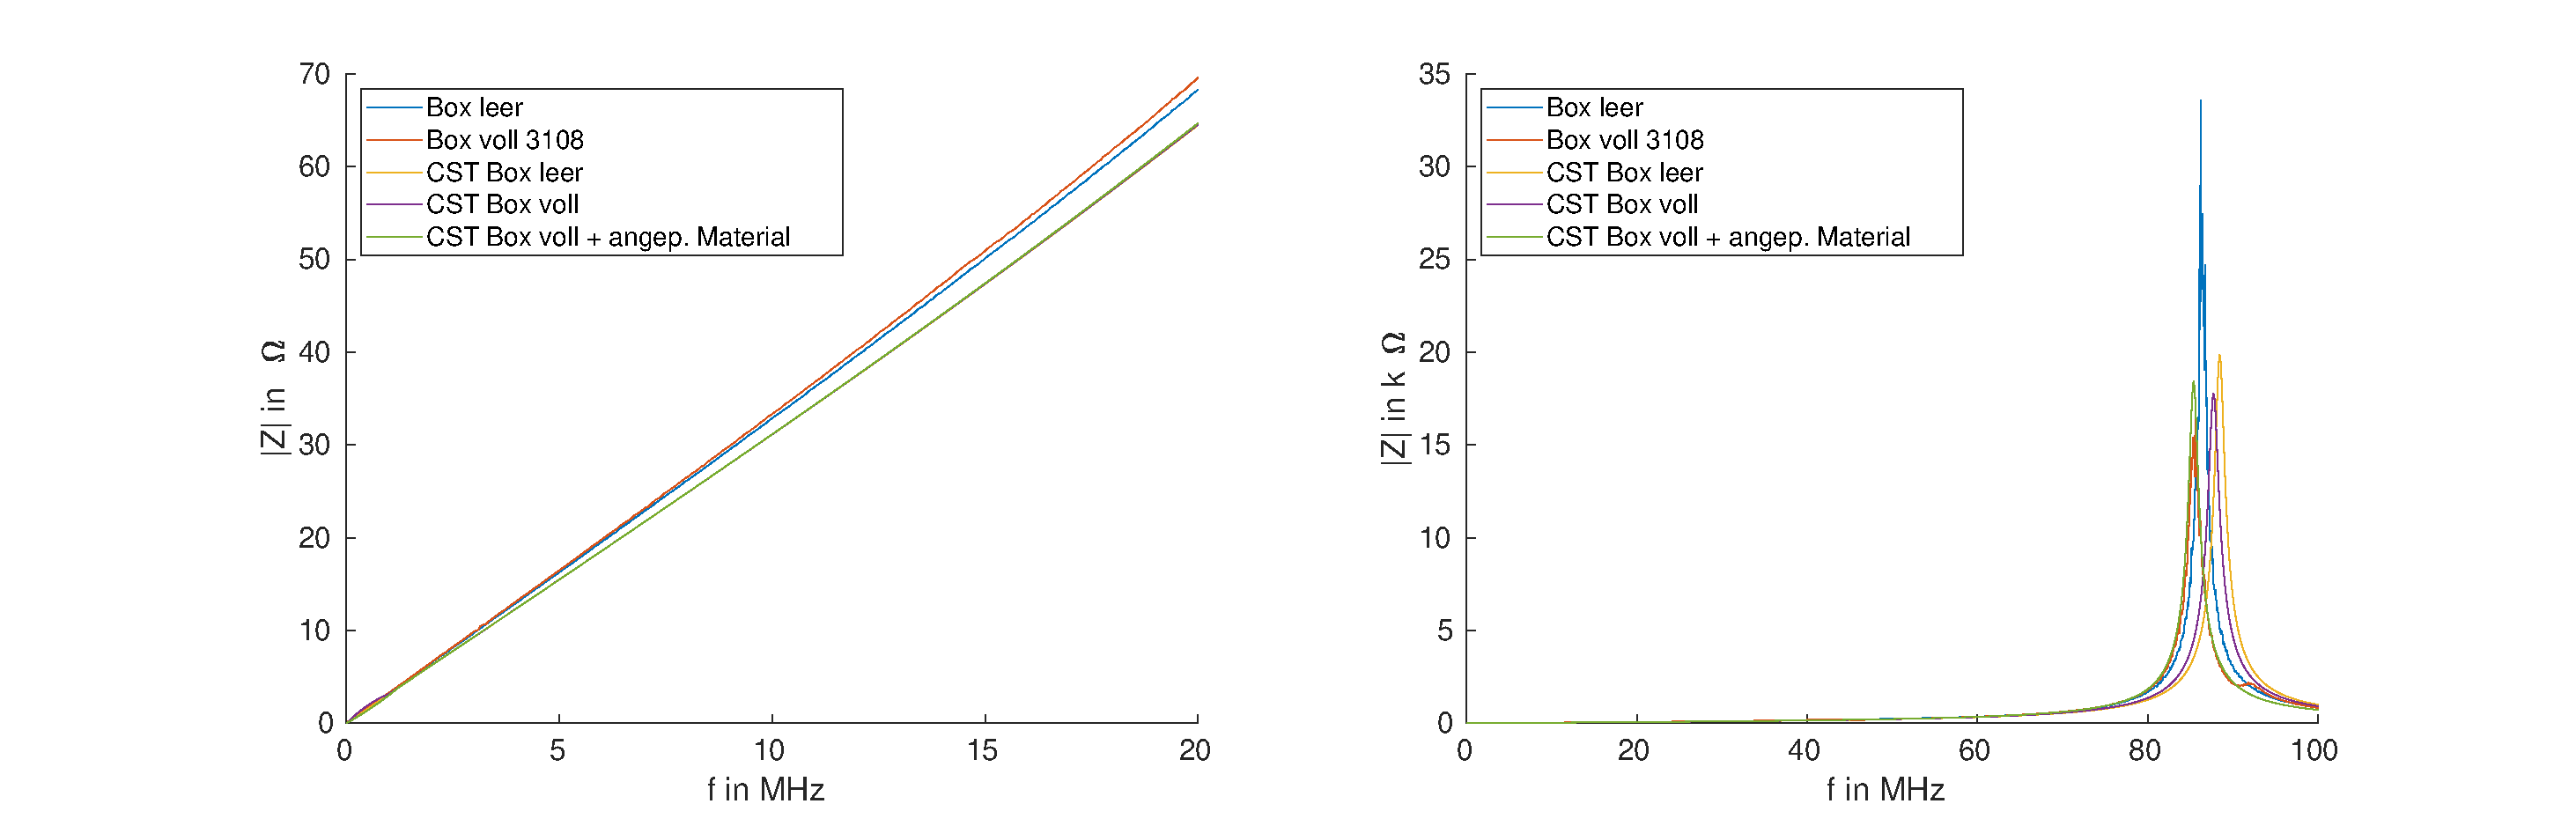
\includegraphics[width=\textwidth]{measurement_simulation_emptybox}
	\caption{Gegen\"uberstellung der Simulation der Box mit Halterung aus Kreuz und Polygon zur entsprechenden Messung.}
	\label{fig:boxpolycross}
\end{figure}

Mit Hilfe von Abbildung~\ref{fig:boxpolycross} können zunächst Messung und Simulation auf Plausibilität überprüft werden.\\
Die Resonanzfrequenz $f_r = \frac{1}{2\pi \cdot \sqrt{LC}}$ eines LC-Schwingkreise sinkt mit steigendem $\varepsilon_r$, da hierdurch die Kapazität erhöht wird. Je mehr Einbauten der Testbox hinzugefügt werden, desto größer kann $\varepsilon_r$ einer Ersatzkapazit\"at angesehen werden, wodurch die Resonanz zu niedrigeren Frequenzen hin verschoben wird.\\
Außerdem zeigt die Abbildung, wie die Simulation durch die Veränderung von $\varepsilon_r$ der Holzkonstruktion mit der Messung besser in Übereinstimmung gebracht werden konnte. Es wurde hierbei vornehmlich $\varepsilon_r'$ variiert. Dieser Vorgehensweise liegt die Annahme zugrunde, dass das verwendete Material in der Testbox mit den für die Simulation hinterlegten Werten übereinstimmt.
\par
Als n\"achstes ist das Modell mit eingesetztem Ringkern zu evaluieren. Dazu wird der Ringkern f\"ur die Simulation auf der Position um den Trovidur Ring gelegt, um die reale Box genau abzubilden. Der Aufbau ist in Abbildung~\ref{fig:RKFeRingCST} gezeigt. Auch hierbei wird wieder die gemessene Impedanz an der Einkopplung direkt mit der Impedanz aus der Simulation gegen\"ubergestellt. Diese Auswertung ist in Abbildung~\ref{fig:boxpolycrossrk} zu sehen.



\newpage



\begin{figure}[htb]
	\centering
	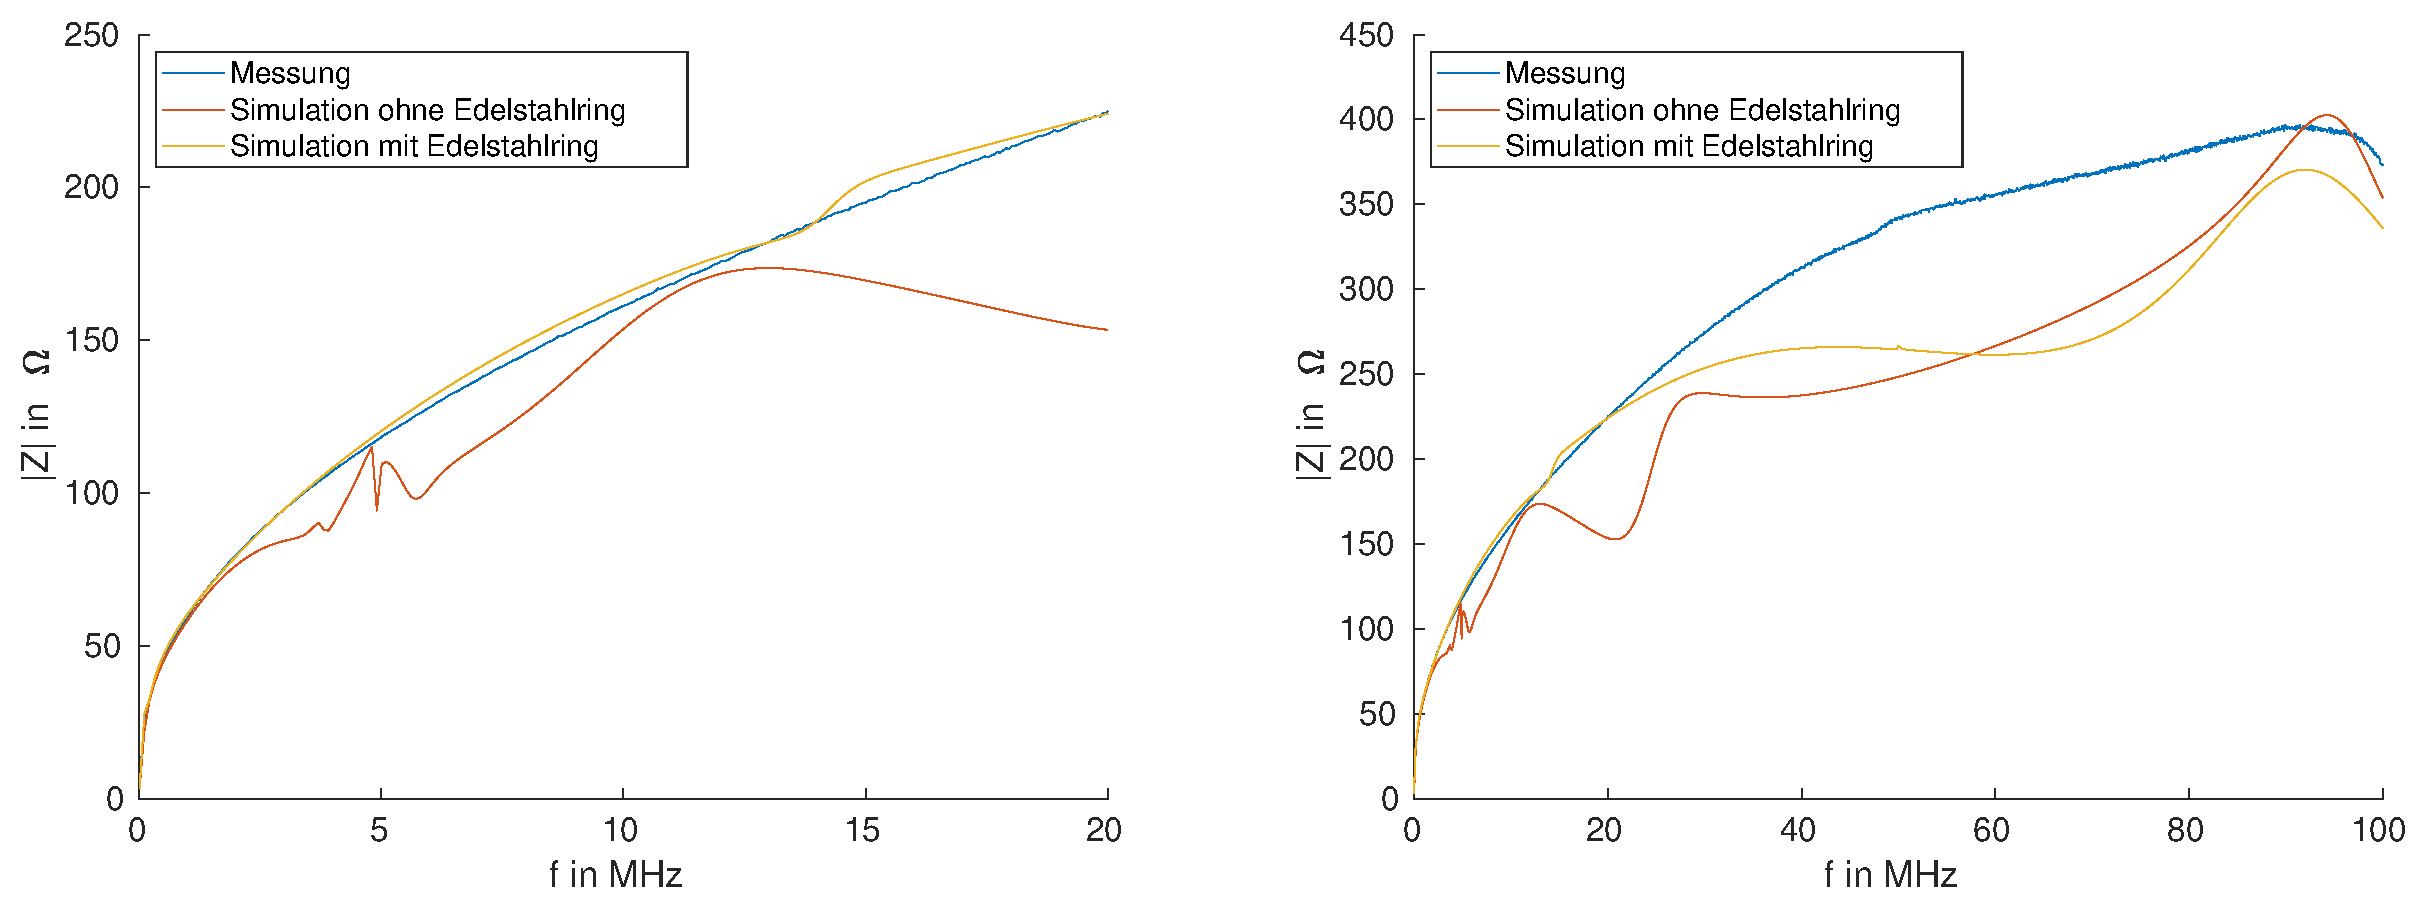
\includegraphics[width=\textwidth]{Zges_RK_SimMeas}
	\caption{Gegen\"uberstellung der gemessenen, mit der simulierten Ringkernimpedanz ohne Kurzschl\"usse}
	\label{fig:boxpolycrossrk}
\end{figure}

F\"ur die erste Simulation wurde sowohl der Ringkern als auch die Halterung dissipativ modelliert. In den CST-Einstellungen wurde das Adaptive Mesh Refinement ausgeschaltet und eine fixe Meshgr\"o\ss{}e von rund $3\cdot10^6$ Meshzellen verwendet. Die Simulation zeigt eine gewisse Welligkeit und nach wie vor eine Abweichung zur Messung. Diese Abweichung konnte bis $\SI{20}{\mega\hertz}$ minimiert werden indem die Ringkernhaltung durch Edelstahl mit $\mu_r = 1$ modeliert.
Dieses Vorgehen wurde jedoch nicht für die weiteren Kurzschluss-Simulationen angewendet (siehe \ref{sec:rksimulation}). 
% \par
% Die Gegen\"uberstellung wird f\"ur alle in Abschnitt~\ref{sec:testbox} genannten Kurzschlussanordnungen in gleicher Form durchgef\"uhrt.
% Es zeigt sich schnell, dass insbesondere im niedrigen Frequenzbereich eine sehr geringe Abweichung zu erkennen ist. Die Mittlere Abweichung zwischen Simulation und Messung liegt unterhalb von $\SI{20}{\mega\hertz}$ bei nur 

% \todo[inline,color=red!30]{wert und ggf Rechnung einf\"ugen}.  
\par
Auch die Kurzschlussmessungen wurden mit der Simulation gegen\"ubergestellt. Zun\"achst wird die Anordnung mit nur einem Kurzschluss betrachtet. Insbesondere im Bereich bis $\SI{50}{\mega\hertz}$ ist eine hohe \"Ubereinstimmung zu sehen. Lediglich im h\"oheren Frequenzbereich, nahe der Resonanz, weichen Messung und Simulation voneinander ab. Abbildung~\ref{fig:boxpolycrossrk1ks} zeigt die Gegen\"uberstellung.

\begin{figure}[htb]
	\centering
	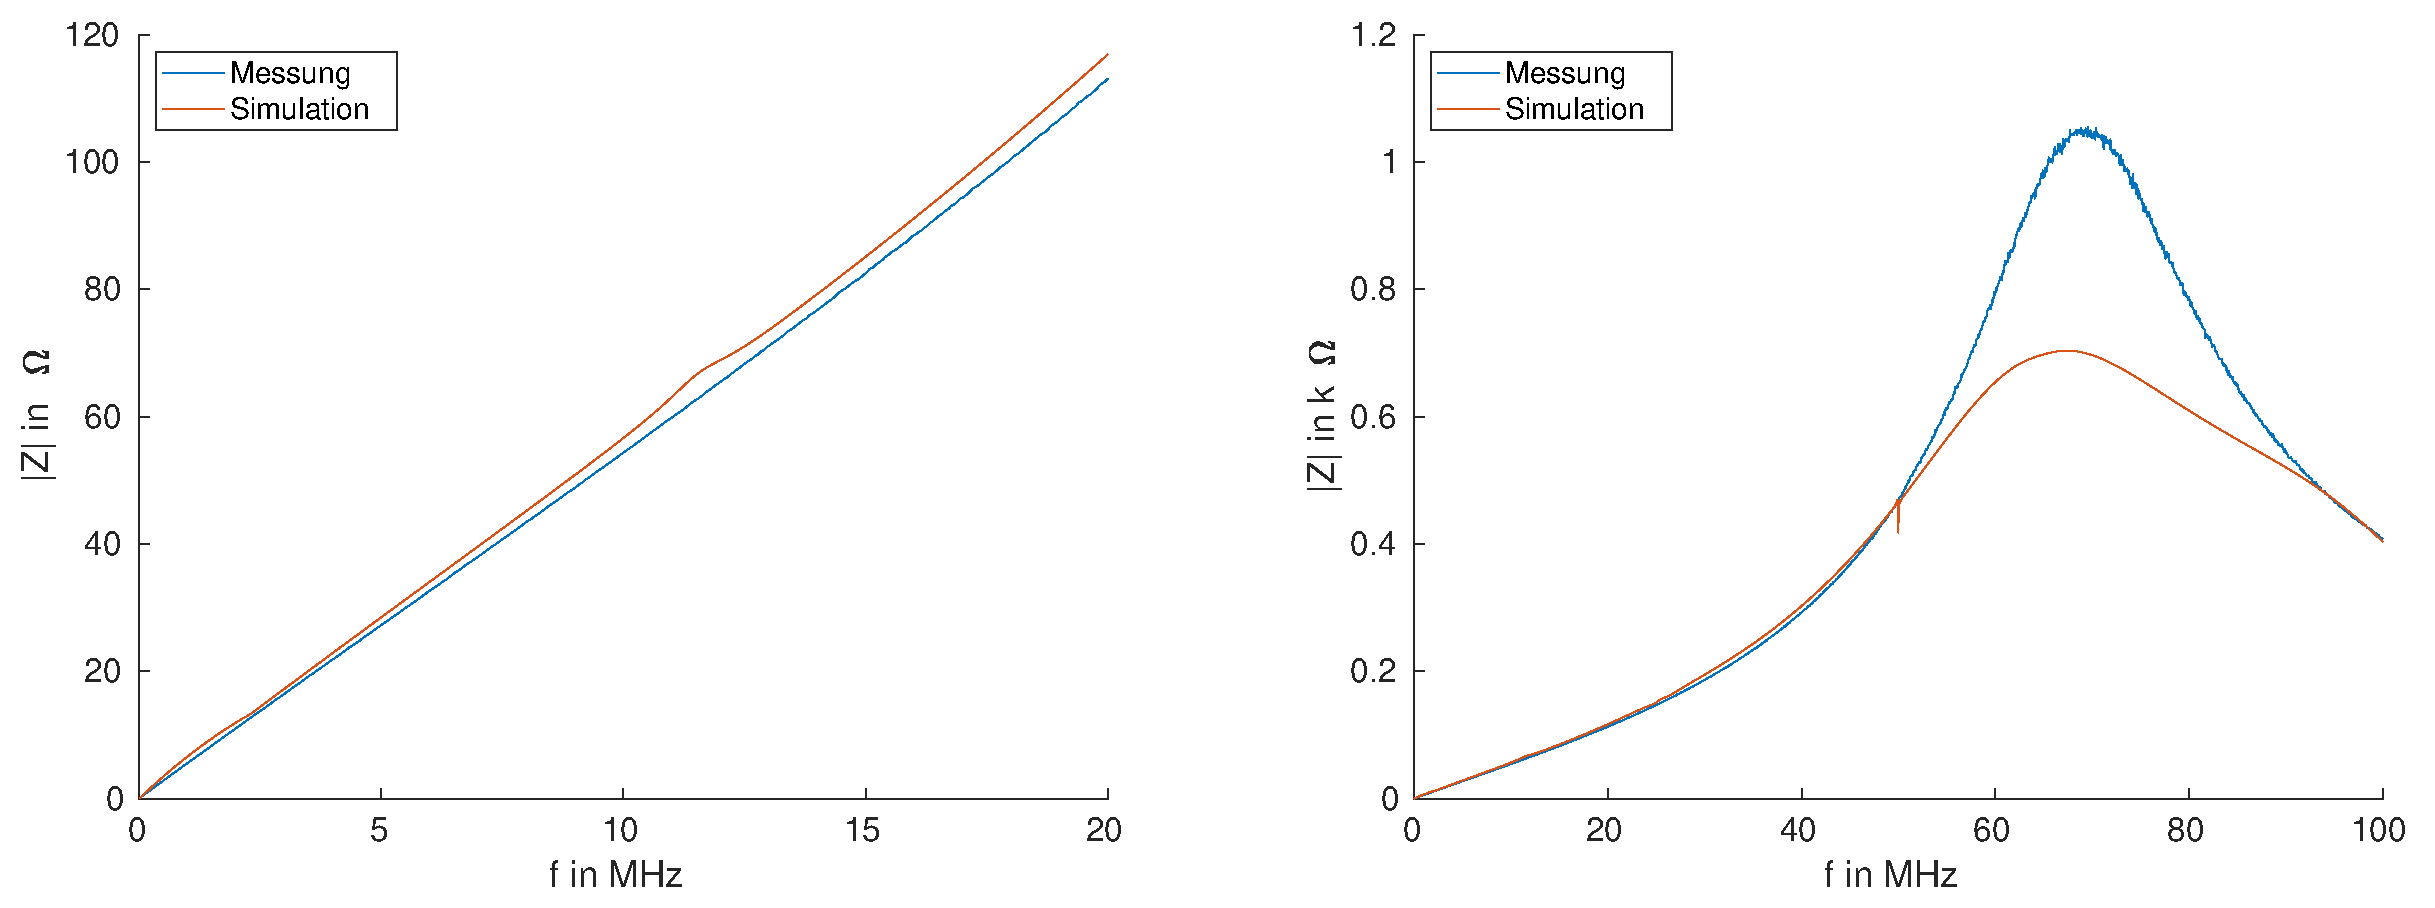
\includegraphics[width=\textwidth]{Z_ges_1KS_SimMeas}
	\caption{Gegen\"uberstellung der gemessenen, mit der simulierten Ringkernimpedanz f\"ur einen Kurzschluss.}
	\label{fig:boxpolycrossrk1ks}
\end{figure}



\newpage



Die Simulation der weiteren Kurzschl\"ussanordnungen zeigt, dass je mehr Kurzschlüsse simuliert werden, die Abweichung zur Messung steigt. Abbildung~\ref{fig:boxpolycrossrk7ks} zeigt diesen Effekt beispielhaft f\"ur eine Anzahl von sieben Kurzschl\"ussen.

\begin{figure}[htb]
	\centering
	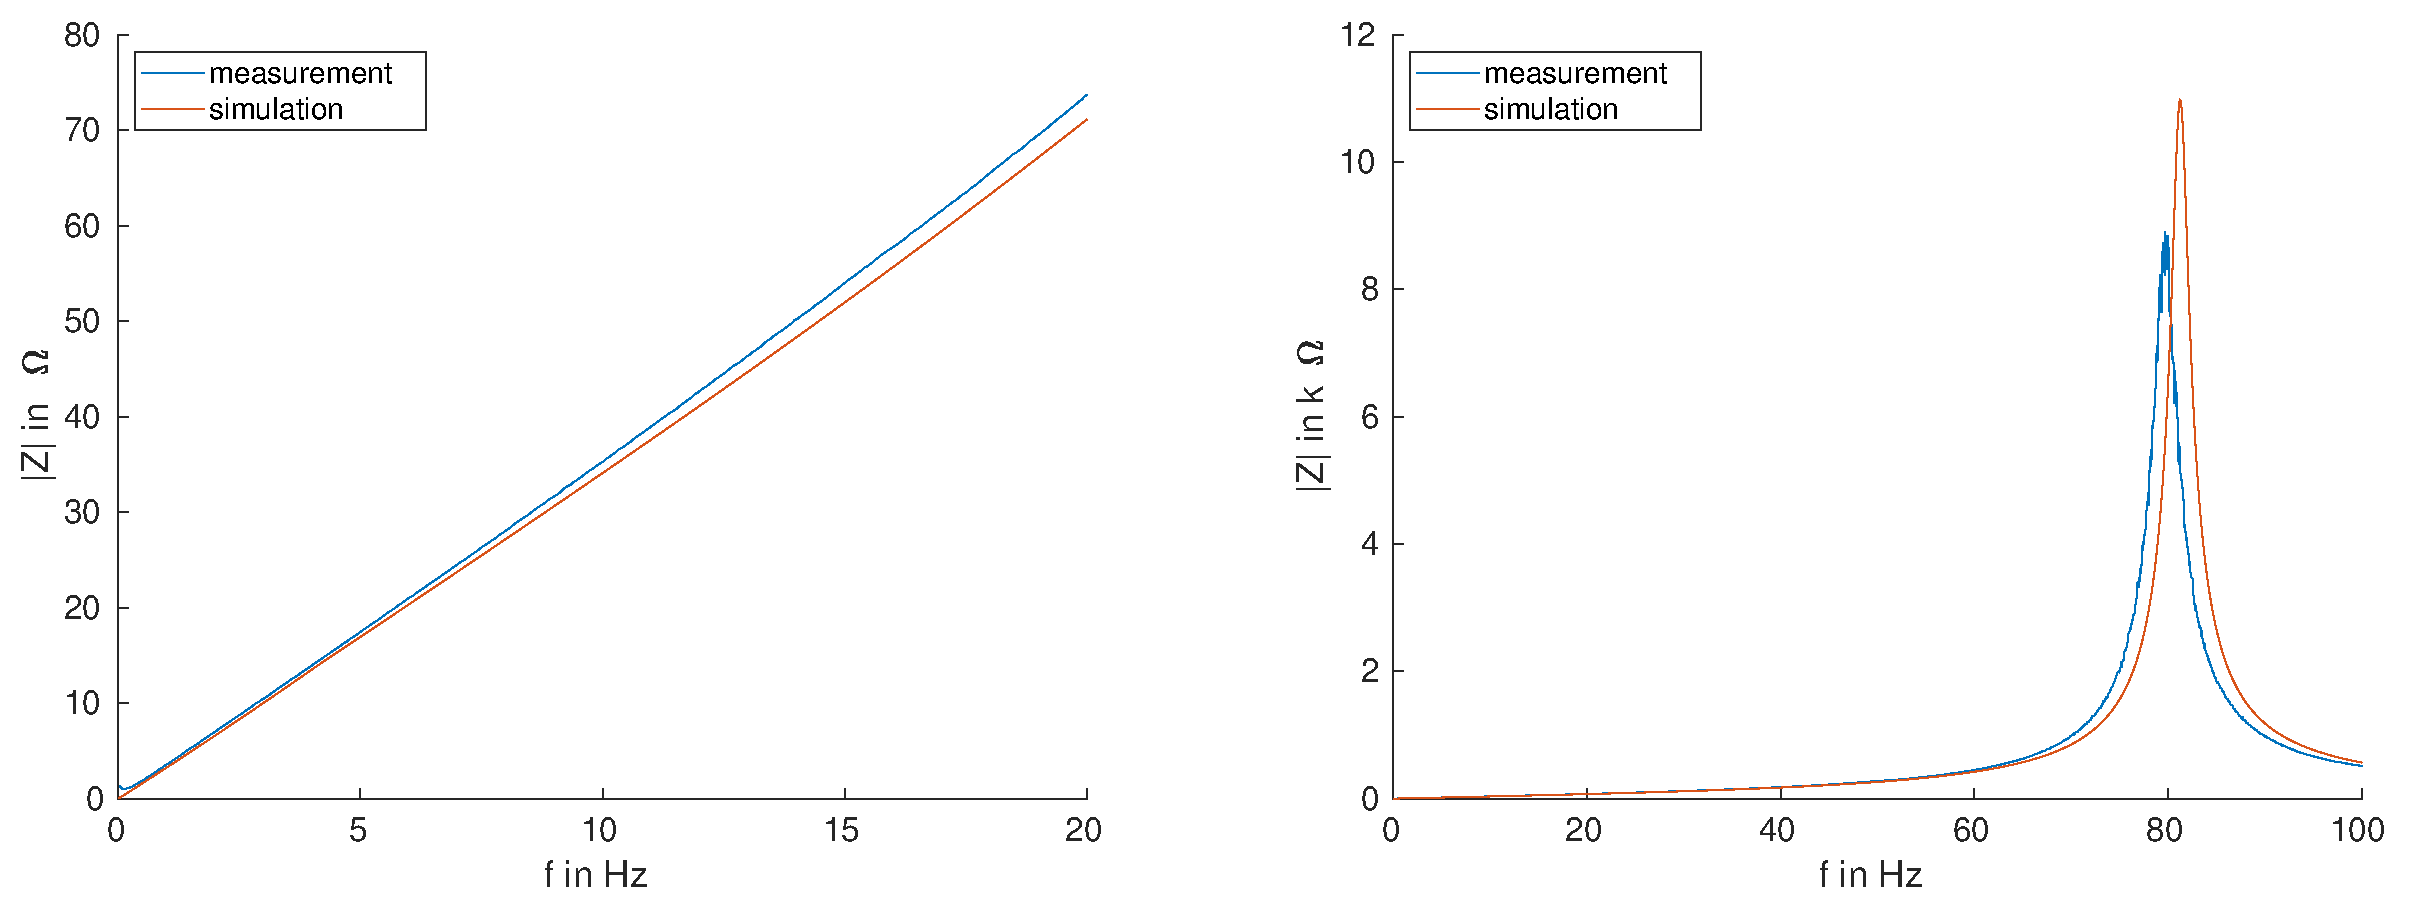
\includegraphics[width=\textwidth]{Z_ges_7KS_SimMeas}
	\caption{Gegen\"uberstellung der gemessenen, mit der simulierten Ringkernimpedanz f\"ur eine Anzahl von sieben Kurzschl\"ussen}
	\label{fig:boxpolycrossrk7ks}
\end{figure}

Eine m\"ogliche Erkl\"arung daf\"ur w\"are, dass die simulierten Kurzschl\"usse idealere Materialeigenschaften, bessere Kontaktierung sowie eine h\"ohere Formsicherheit aufweisen, als es das Kupfer und die Verschraubung in der Realit\"at liefern k\"onnen. Die Gegen\"uberstellung aller Kurzschlussanordnungen in Simulation und Messung sind in Anhang~\ref{sec:simmesskomplett} abgebildet.


\section{Auswertung der Kurzschlussanordnungen}
Nachdem die Messungen, sowie die Simulationen gegeneinander abgeglichen sind, kann die Auswertung der Kurzschlussversuche begonnen werden. Dazu wird nur die reine Ringkernimpedanz betrachtet und nach der Beschreibung in Kapitel~\ref{chap:simulation} berechnet. Analog zum in Abschnitt~\ref{sec:ringkern} beschriebenen Vorgehen, wird auch hierzu die Impedanz $Z_{rk}$ aus der gemessenen Impedanz $Z_{ges}$ nach Gleichung~\ref{eq:Zrk} herausgerechnet. Somit l\"asst sich isoliert betrachten, wie viel Anteil der Ringkernimpedanz durch das Hinzuf\"ugen der Kurzschl\"usse noch verbleibt. Dazu  werden die in Unterkapitel~\ref{sec:shorts} angef\"uhrten Variationsparameter gegenübergestellt.
\par
Für die Auswertung werden die Impedanzmesswerte in Relation zur Impedanz der Testbox ohne Kurzschlüsse gesetzt. Die prozentuale Abweichung kann dann wie folgt berechnet und für verschiedene Variationen verglichen werden.
\begin{equation}
	\delta Z_{prozentual}(f) = \frac{Z_{rk}(f) - Z_{var}(f)}{Z_{rk}(f)}\cdot 100 = \left(1-\frac{Z_{var}(f)}{Z_{rk}(f)}\right)\cdot 100
	\label{eq:maxdiffpercent}
\end{equation}
In der folgenden Ausführung wird für $Z_{var}$ die Impedanz des zu betrachtenden Parameters eingesetzt. $Z_{rk}$ bezeichnet die Impedanz des Ringkerns ohne Kurzschl\"usse.

\subsection{Anzahl der Kurzschl\"usse}
Um den Einfluss verschiedener Anzahlen an Kurzschl\"ussen zu analysieren, werden ein bis acht identische Kurzschl\"usse in der Testbox montiert. Abbildung~\ref{fig:ringcorenumberCST} zeigt die Positionen der montierten Kurzschl\"usse.

\begin{figure}[htb]
	\centering
	\subfloat{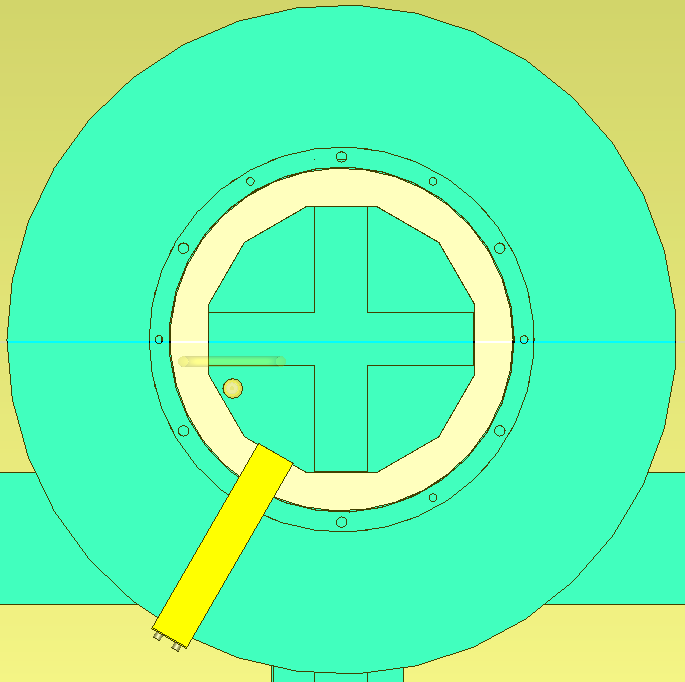
\includegraphics[height=0.24\textwidth]{1ksb30}}
	\hspace{0.0065\textwidth}
	\subfloat{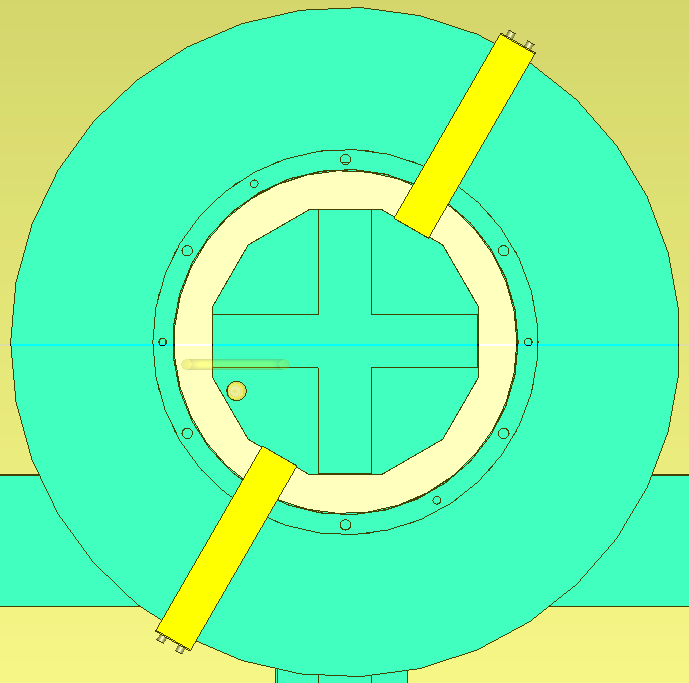
\includegraphics[height=0.24\textwidth]{2ksb30}}
	\hspace{0.0065\textwidth}
	\subfloat{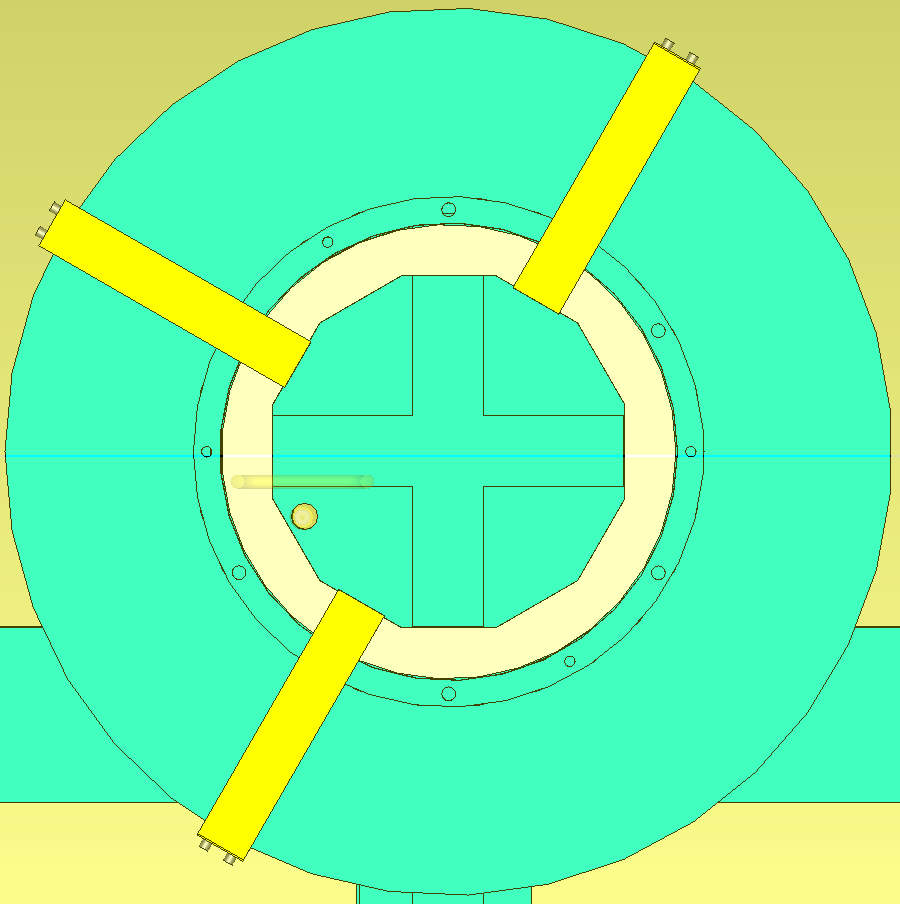
\includegraphics[height=0.24\textwidth]{3ksb30}}
	\hspace{0.0065\textwidth}
	\subfloat{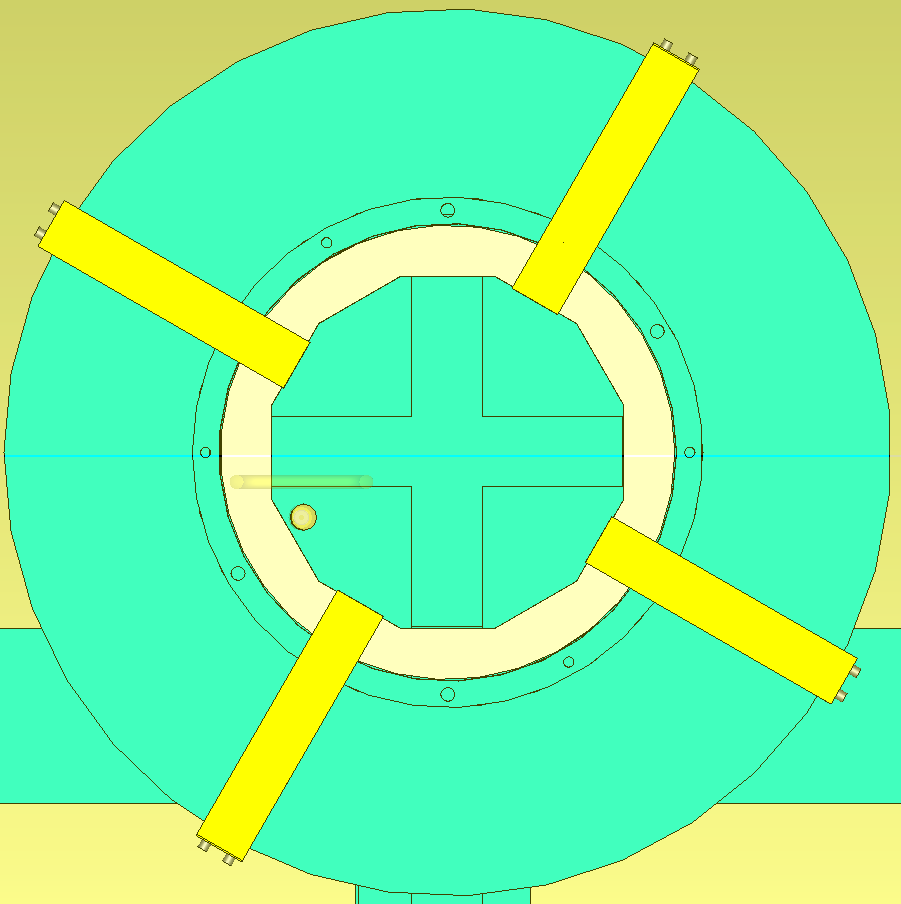
\includegraphics[height=0.24\textwidth]{4ksb30}}
	\\
	\subfloat{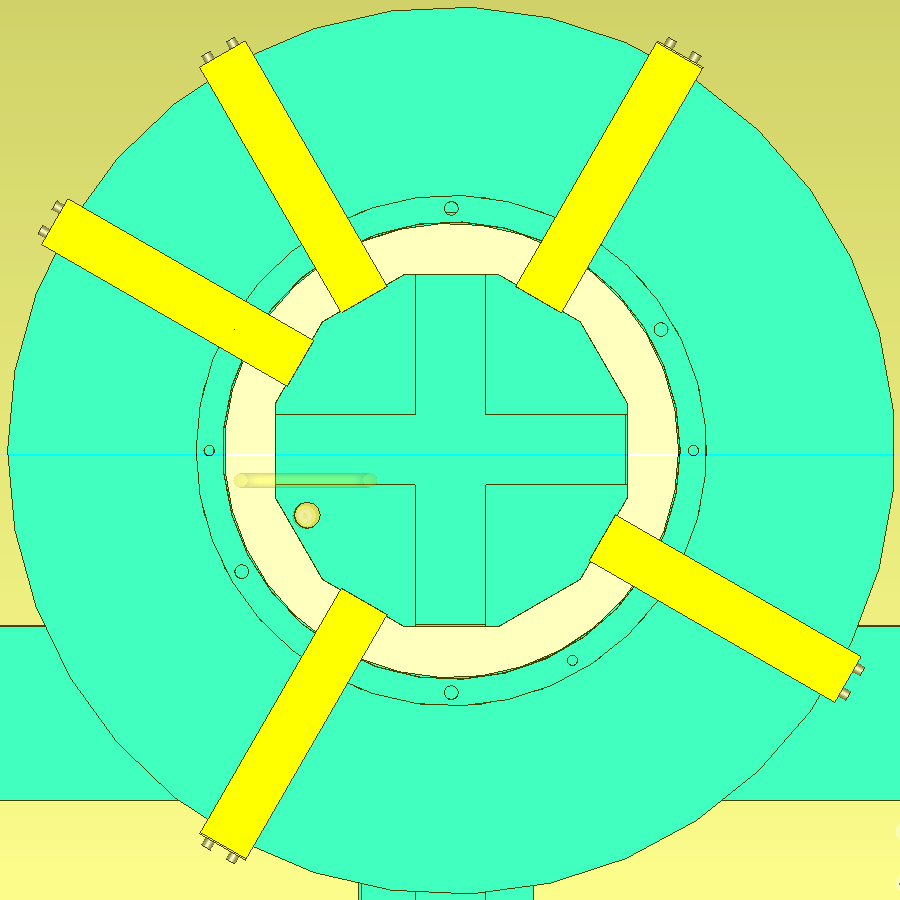
\includegraphics[height=0.24\textwidth]{5ksb30}}
	\hspace{0.0065\textwidth}
	\subfloat{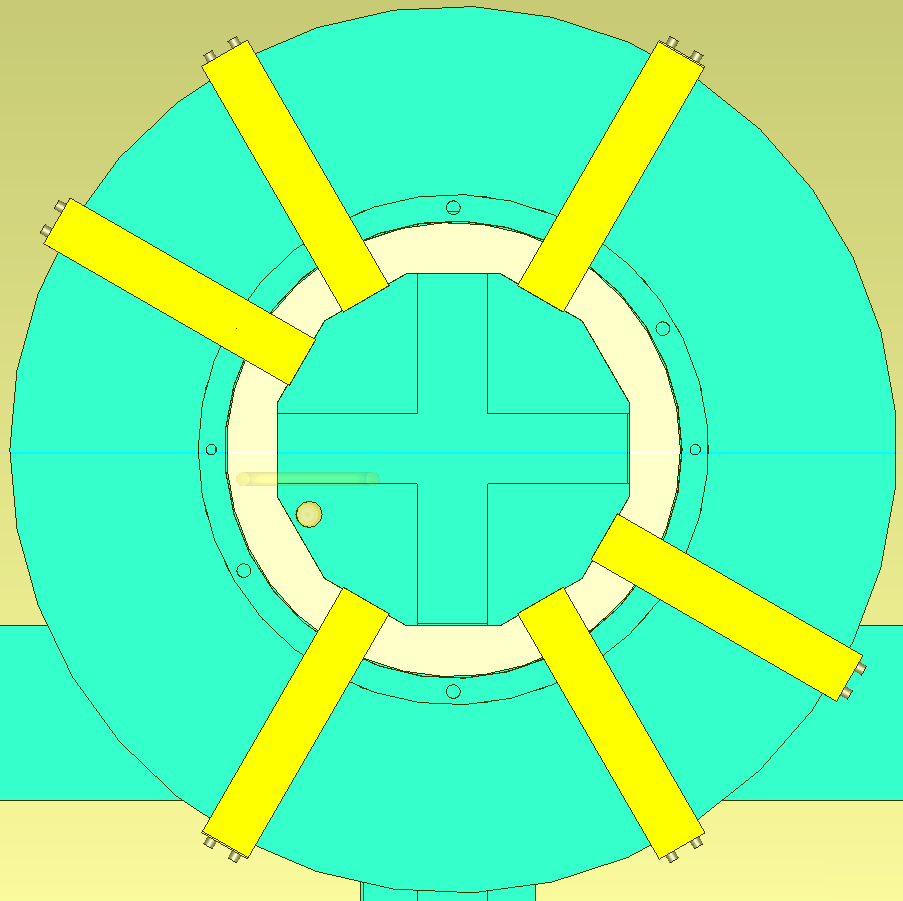
\includegraphics[height=0.24\textwidth]{6ksb30}}
	\hspace{0.0065\textwidth}
	\subfloat{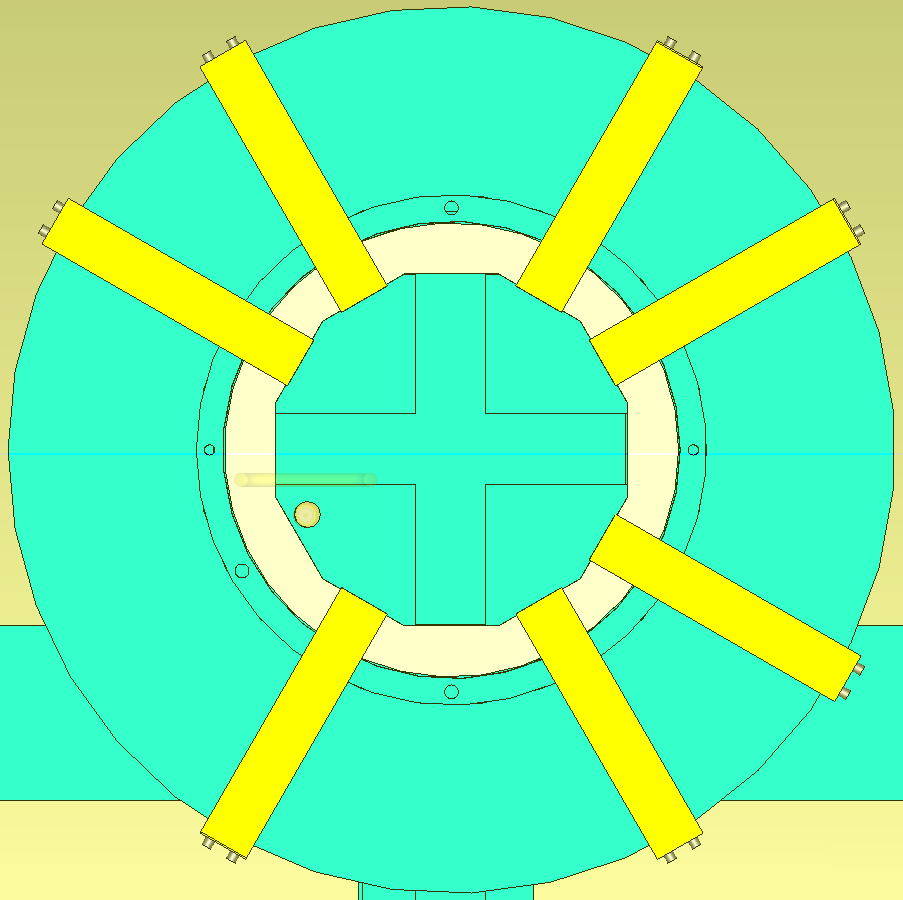
\includegraphics[height=0.24\textwidth]{7ksb30}}
	\hspace{0.0065\textwidth}
	\subfloat{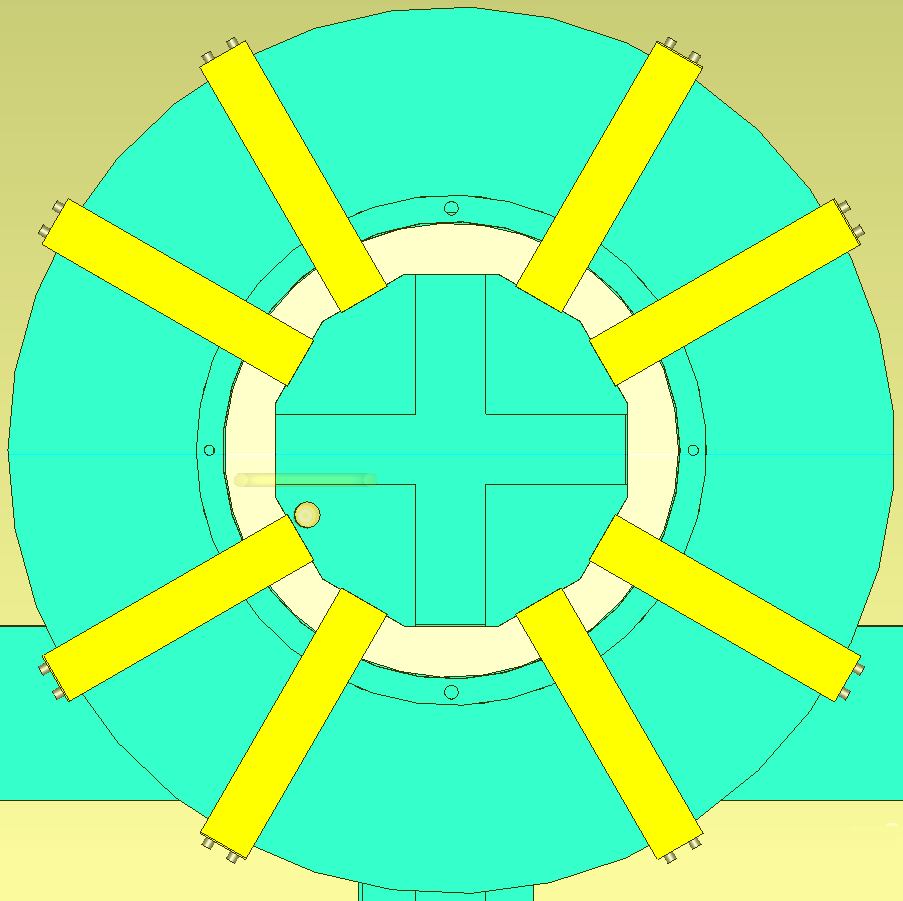
\includegraphics[height=0.24\textwidth]{8ksb30}}
	\caption{Unterschiedliche Anzahlen an montierten Kurzschl\"ussen an verschiedenen Positionen.}
	\label{fig:ringcorenumberCST}
\end{figure}

% \todo[inline,color=red!30]{Erkl\"aren warum 8KS bei der Auswertung nicht mehr auftaucht}  
Die achte Kurzschlusschiene, welche in Grafik~\ref{fig:ringcorenumberCST} zu sehen ist, konnte bei der endg\"ultigen Auswertung nicht ber\"ucksichtigt werden. Dieser Kurzschluss liegt sehr nah am Einkopplungsrohr, sodass ein direkter Kontakt dazu besteht. F\"ugt man einen Abstandshalter aus Schaumstoff zu, so wird die Einkopplung etwas nach oben gebogen. Die Messung liefert daher verf\"alschte Ergebnisse, welche deutlich st\"arker von der Simulation abweichen, als bei anderen Messungen. Auch dieses Verhalten ist in Anhang~\ref{sec:simmesskomplett} abgebildet. F\"ur die endg\"ultige Auswertung wurden folglich nur ein bis sieben Kurzschl\"usse betrachtet. Die resultierende Ringkernimpedanz f\"ur die einzelnen Kurzschlussanordnungen ist in Abbildung~\ref{fig:ringcorenumber} \"uber der Frequenz aufgetragen.


\newpage

\begin{figure}[htb]
	\centering
	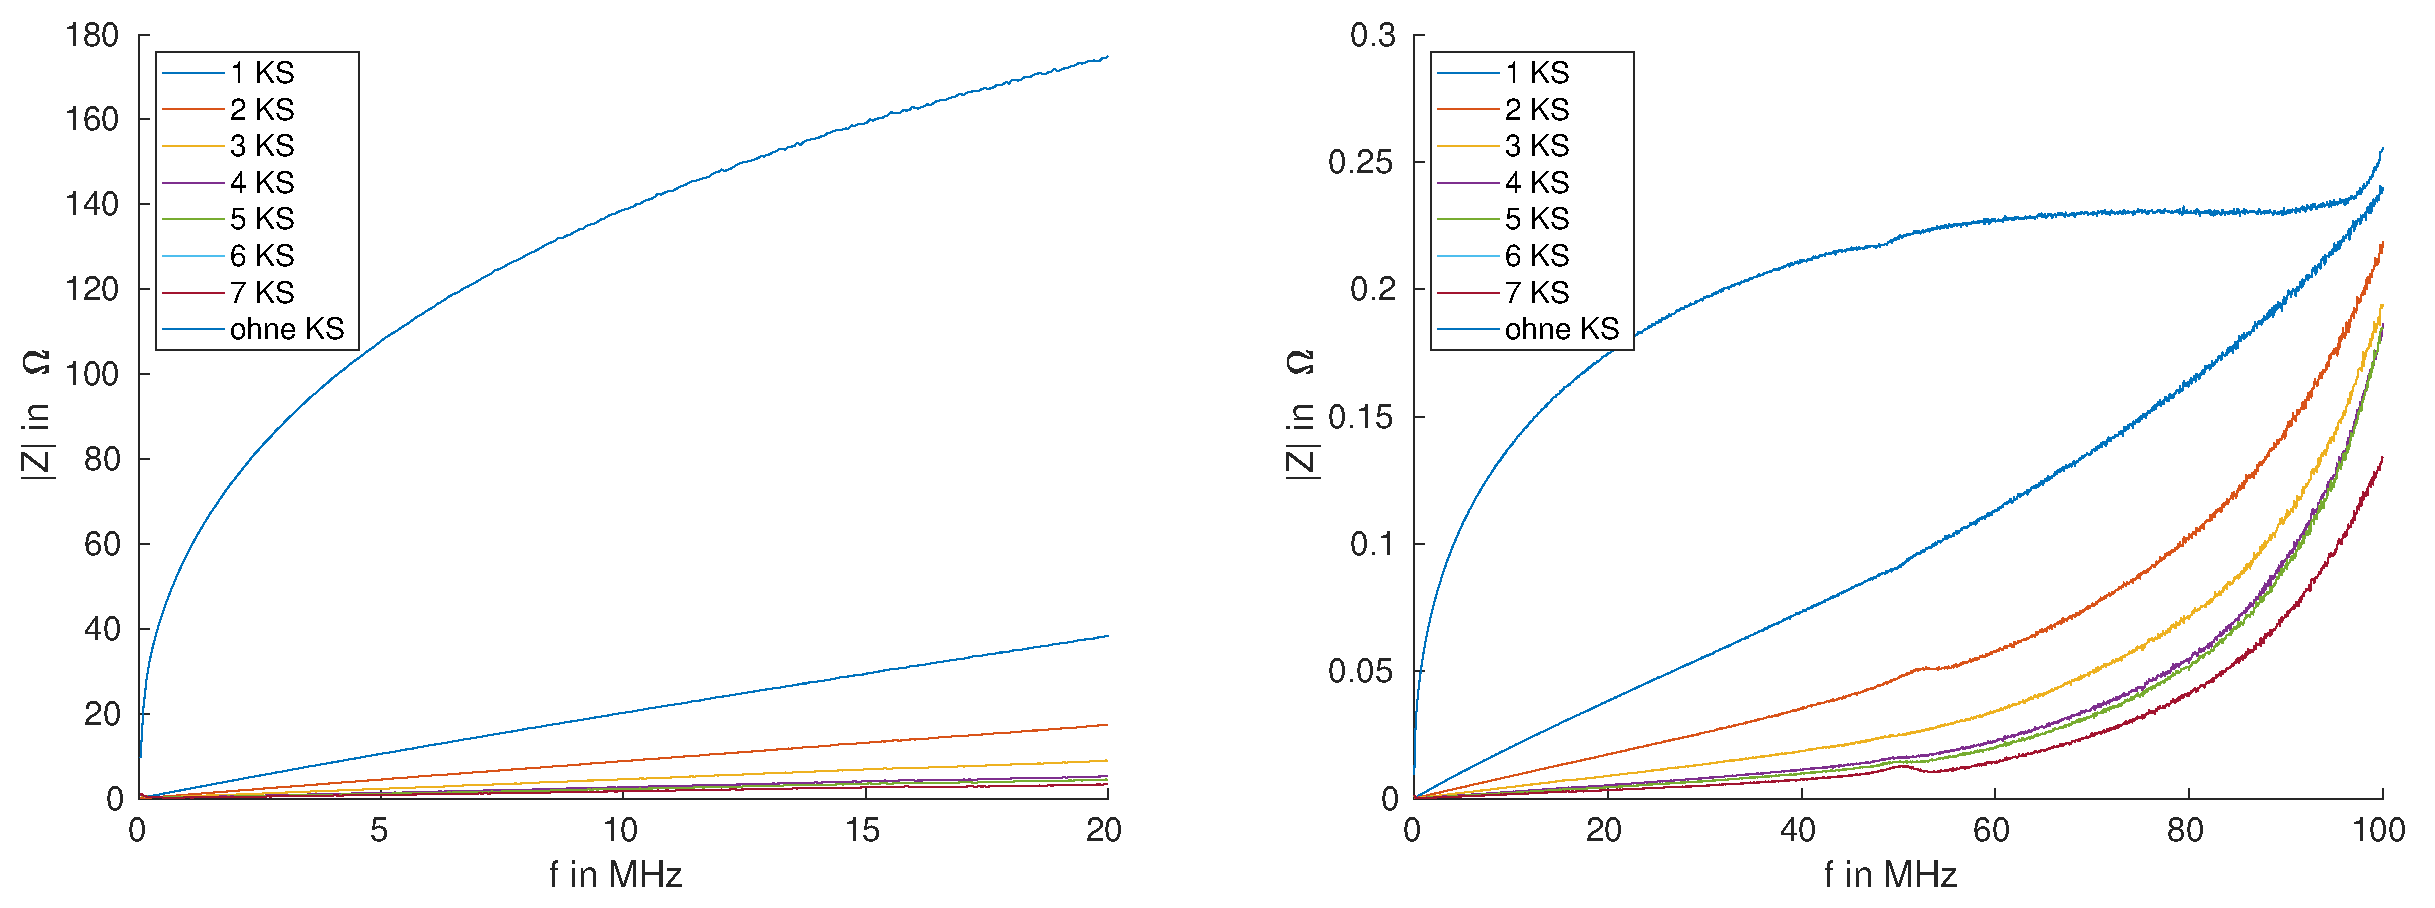
\includegraphics[width=\textwidth]{impedance_numberKS_ringcore}
	\caption{Gegen\"uberstellung der Ringkernimpedanz \"uber der Frequenz f\"ur verschiedene Anzahlen an Kurzschl\"ussen}
	\label{fig:ringcorenumber}
\end{figure}

Es f\"allt auf, dass der gr\"o\ss{}te Unterschied zwischen dem Ringkern ohne Kurzschluss und einem Kurzschluss besteht. Das bedeutet, dass die Montage weiterer Kurzschl\"usse mit zunehmender Anzahl weniger effektiv ist. Dies wird durch die folgenden Betrachtung verdeutlicht, bei die Impedanz an festen Frequenzen ausgewertet und \"uber der Anzahl an Kurzschl\"ussen aufgetragen wird. Dies geschieht bei 5, 10 und $\SI{20}{\mega\hertz}$, da insbesondere der niedrigere Frequenzbereich f\"ur den Beschleunigerbetrieb von Relevanz ist~\citep{frey2015status}. Die Gegen\"uberstellung ist in Abbildung~\ref{fig:ringcorenumber20} aufgetragen.

\begin{figure}[htb]
	\centering
	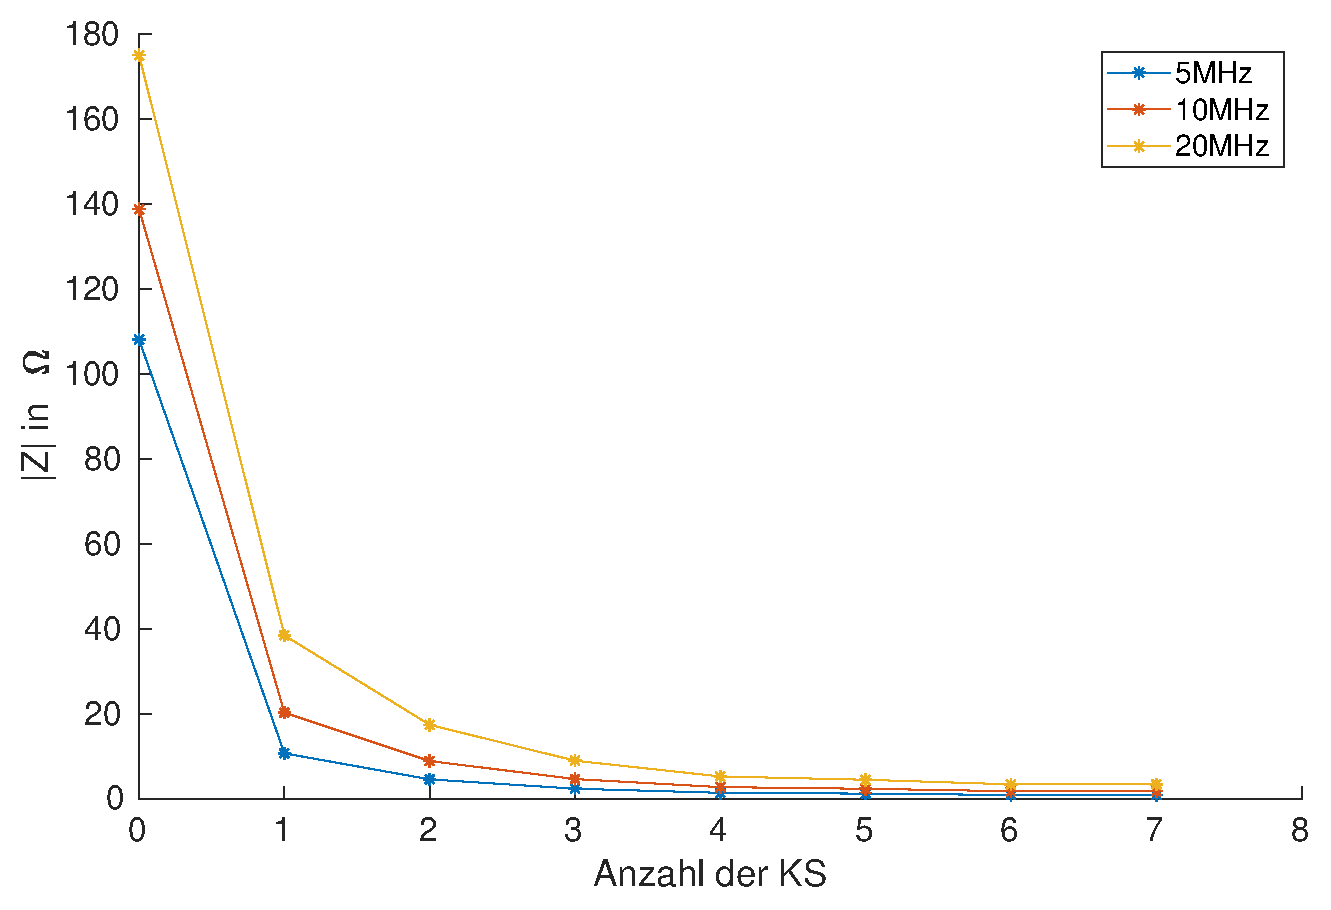
\includegraphics[width=0.5\textwidth]{RK_Impedanz_numberKS_frequenz}
	\caption{Gegen\"uberstellung der Ringkernimpedanz mit verschiedenen Anzahlen an Kurzschl\"ussen bei 5, 10 und $\SI{20}{\mega\hertz}$.}
	\label{fig:ringcorenumber20}
\end{figure}

Wird die Impedanz mit Kurzschlüssen in Relation zur Ringkernimpedanz gesetzt, kann der Effekt der Kurzschl\"usse wie beschrieben dargestellt werden. Für einen Kurzschluss ergibt sich bei \SI{20}{\mega\hertz} somit eine prozentuale Verringerung von 
\begin{equation}
	\frac{\SI{175,1145}{\Omega} - \SI{38,4525}{\Omega}}{\SI{175,1145}{\Omega}}\cdot 100 = \SI{78,042}{\%}.
	\label{eq:maxdiffpercentzeroone}
\end{equation}
Für zwei Kurzschlüsse errechnet nach Formel~\ref{eq:maxdiffpercent} sich eine prozentuale Abweichung von $\SI{90,08}{\%}$, was gegenüber einem Kurzschluss eine weitere Verringerung um $\SI{12,038}{\%}$ bedeutet. Diese weitere Verringerung fällt damit deutlich geringer aus, als es bereits durch einen Kurzschluss der Fall ist. Auch der Vergleich von einem zu sieben Kurzschlüssen, die eine Verringerung der Ringkernimpedanz von $\SI{98,09}{\%}$ hervorrufen, fällt mit weiteren $\SI{20,048}{\%}$ vergleichsweise gering aus.

\subsection{Breite der Kurzschl\"usse}
Die Breite der Kurzschl\"usse ist ein Parameter, welcher durch die schienenartige Form der Kurzschl\"usse leicht zu variieren ist, da diese nur aus einem Blech geschnitten werden. Die montierten Kurzschl\"usse verschiedener Breiten sind in Abbildung~\ref{fig:ringcorewidthCST} abgebildet.

\begin{figure}[htb]
	\centering.
	\subfloat[$\SI{20}{\milli\meter}$]{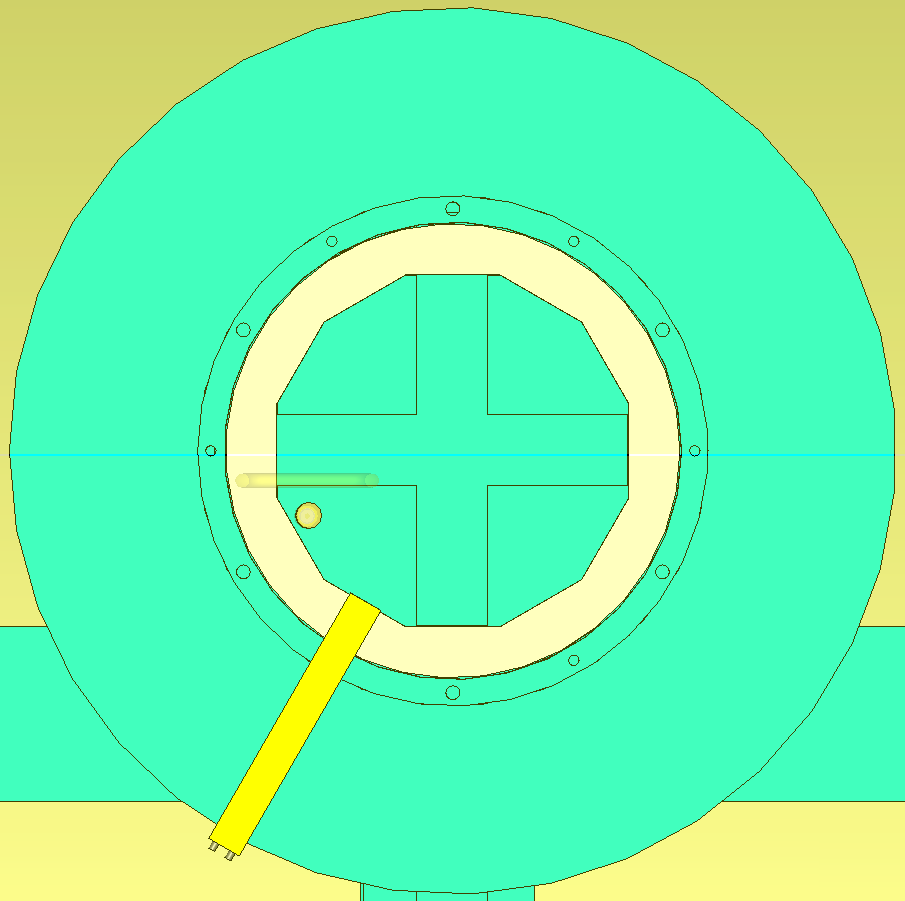
\includegraphics[height=0.3\textwidth]{1ksb20}}
	\hspace{0.02\textwidth}
	\subfloat[$\SI{30}{\milli\meter}$]{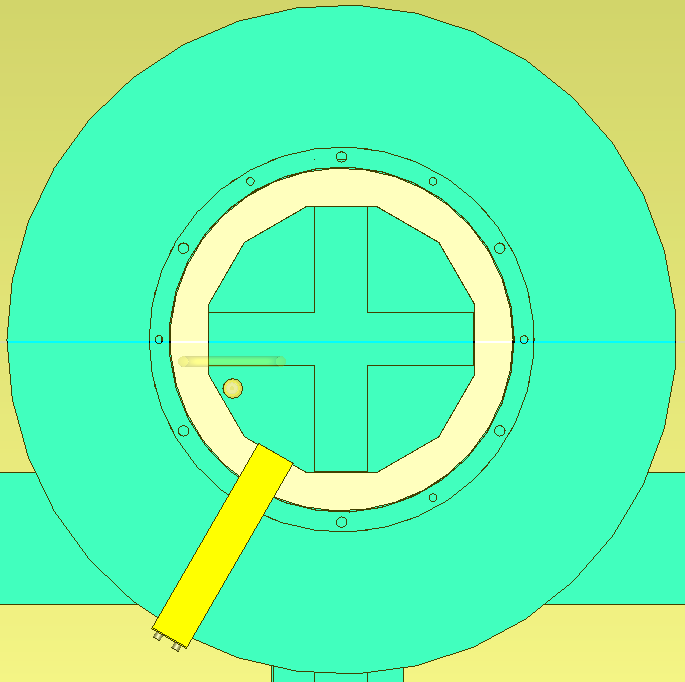
\includegraphics[height=0.3\textwidth]{1ksb30}}
	\hspace{0.02\textwidth}
	\subfloat[$\SI{50}{\milli\meter}$]{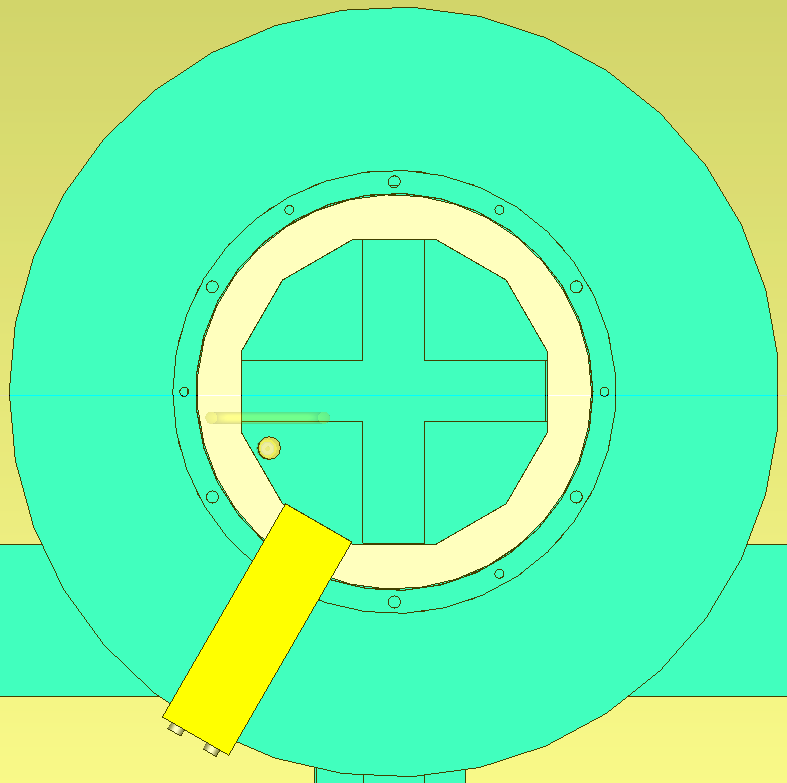
\includegraphics[height=0.3\textwidth]{1ksb50}}
	\caption{Jeweils ein montierter Kurzschluss mit verschiedenen Breiten.}
	\label{fig:ringcorewidthCST}
\end{figure}



\newpage



Da eine h\"ohere Anzahl an Kurzschl\"ussen eine verringerte Ringkernimpedanz als Ergebnis liefert, liegt die Vermutung nahe, dass auch breitere Kurzschl\"usse die Ringkernimpedanz weiter verringern k\"onnen. Die Gegen\"uberstellung der Ringkernimpedanz $Z_{rk}$ ist in Abbildung~\ref{fig:ringcorewidth} zu sehen.

\begin{figure}[htb]
	\centering
	\subfloat[1 Kurzschluss]{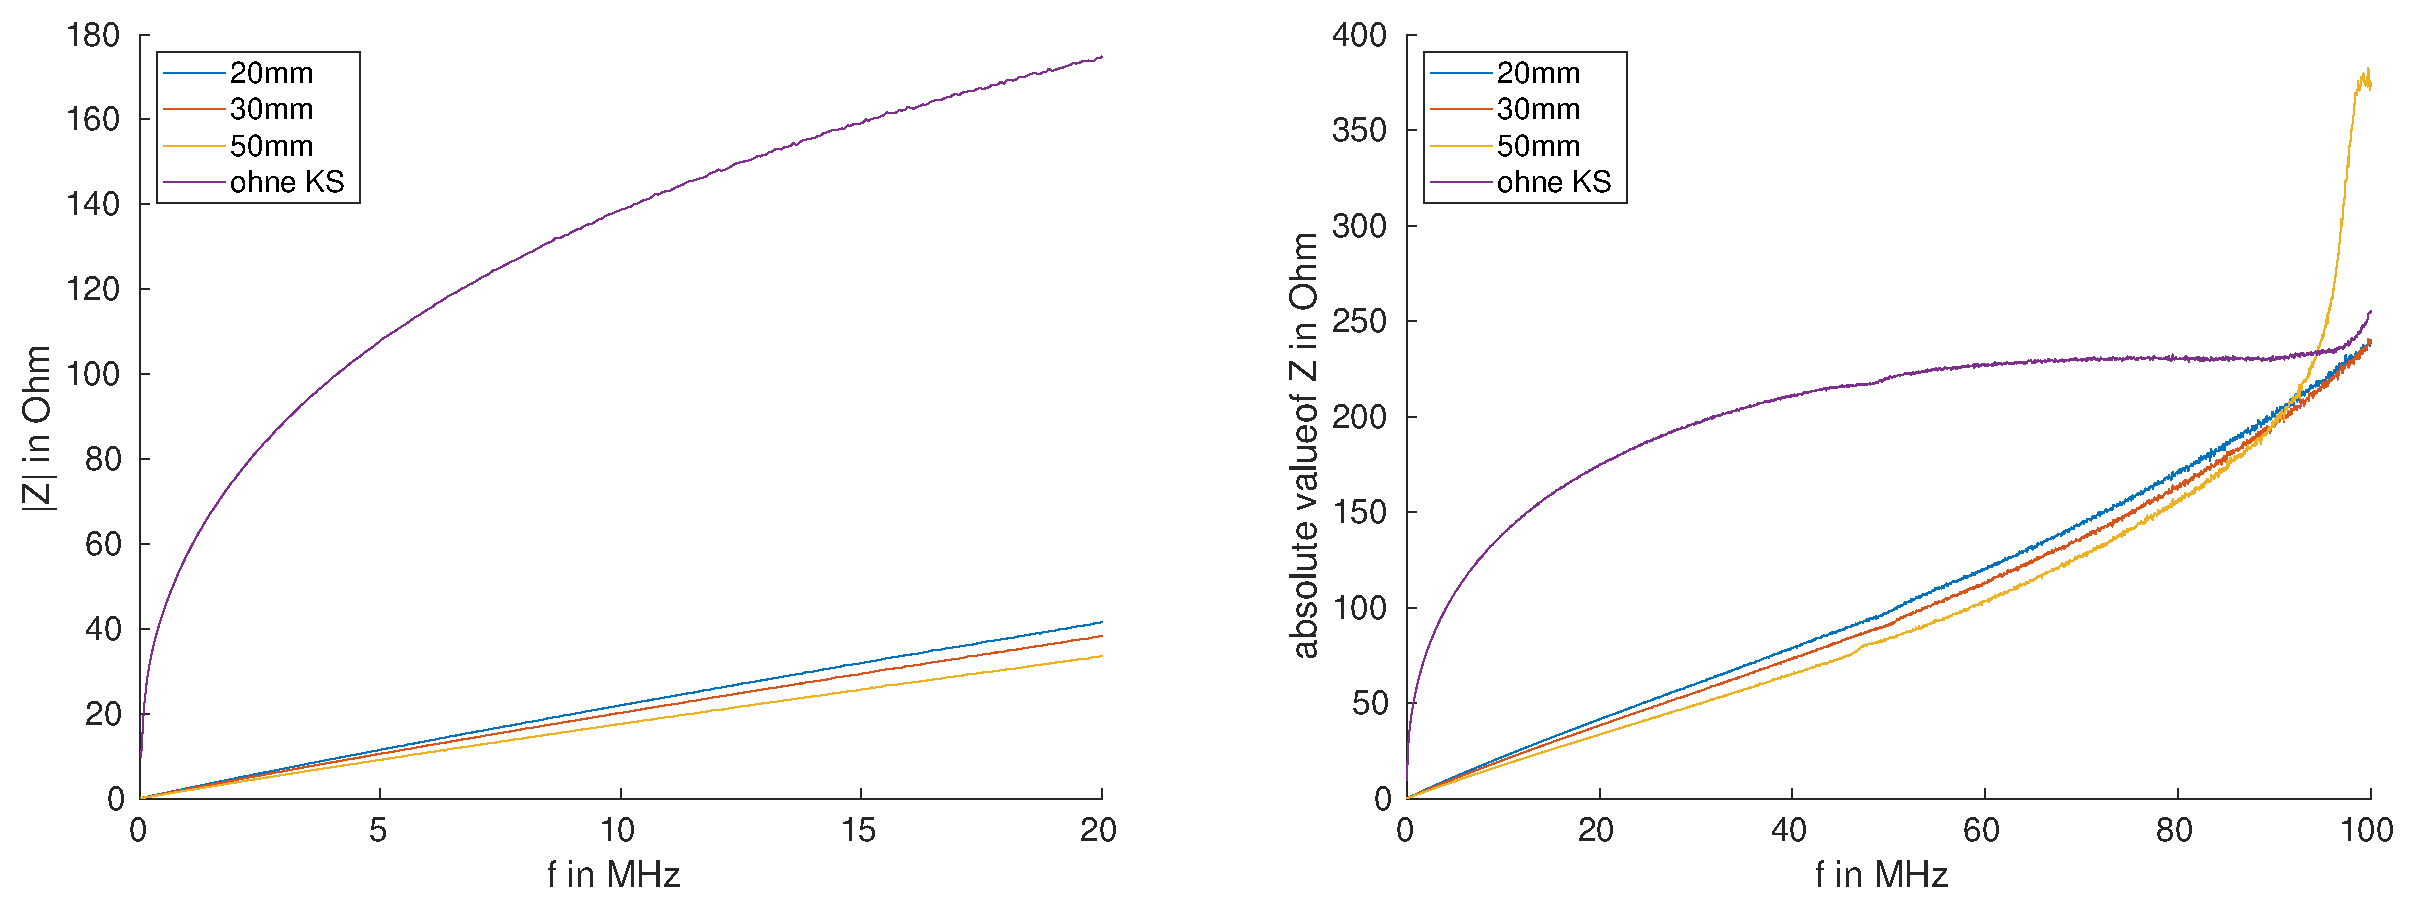
\includegraphics[width=\textwidth]{Z_RK_width_1KS}}
	\\
	\subfloat[2 Kurzschl\"usse]{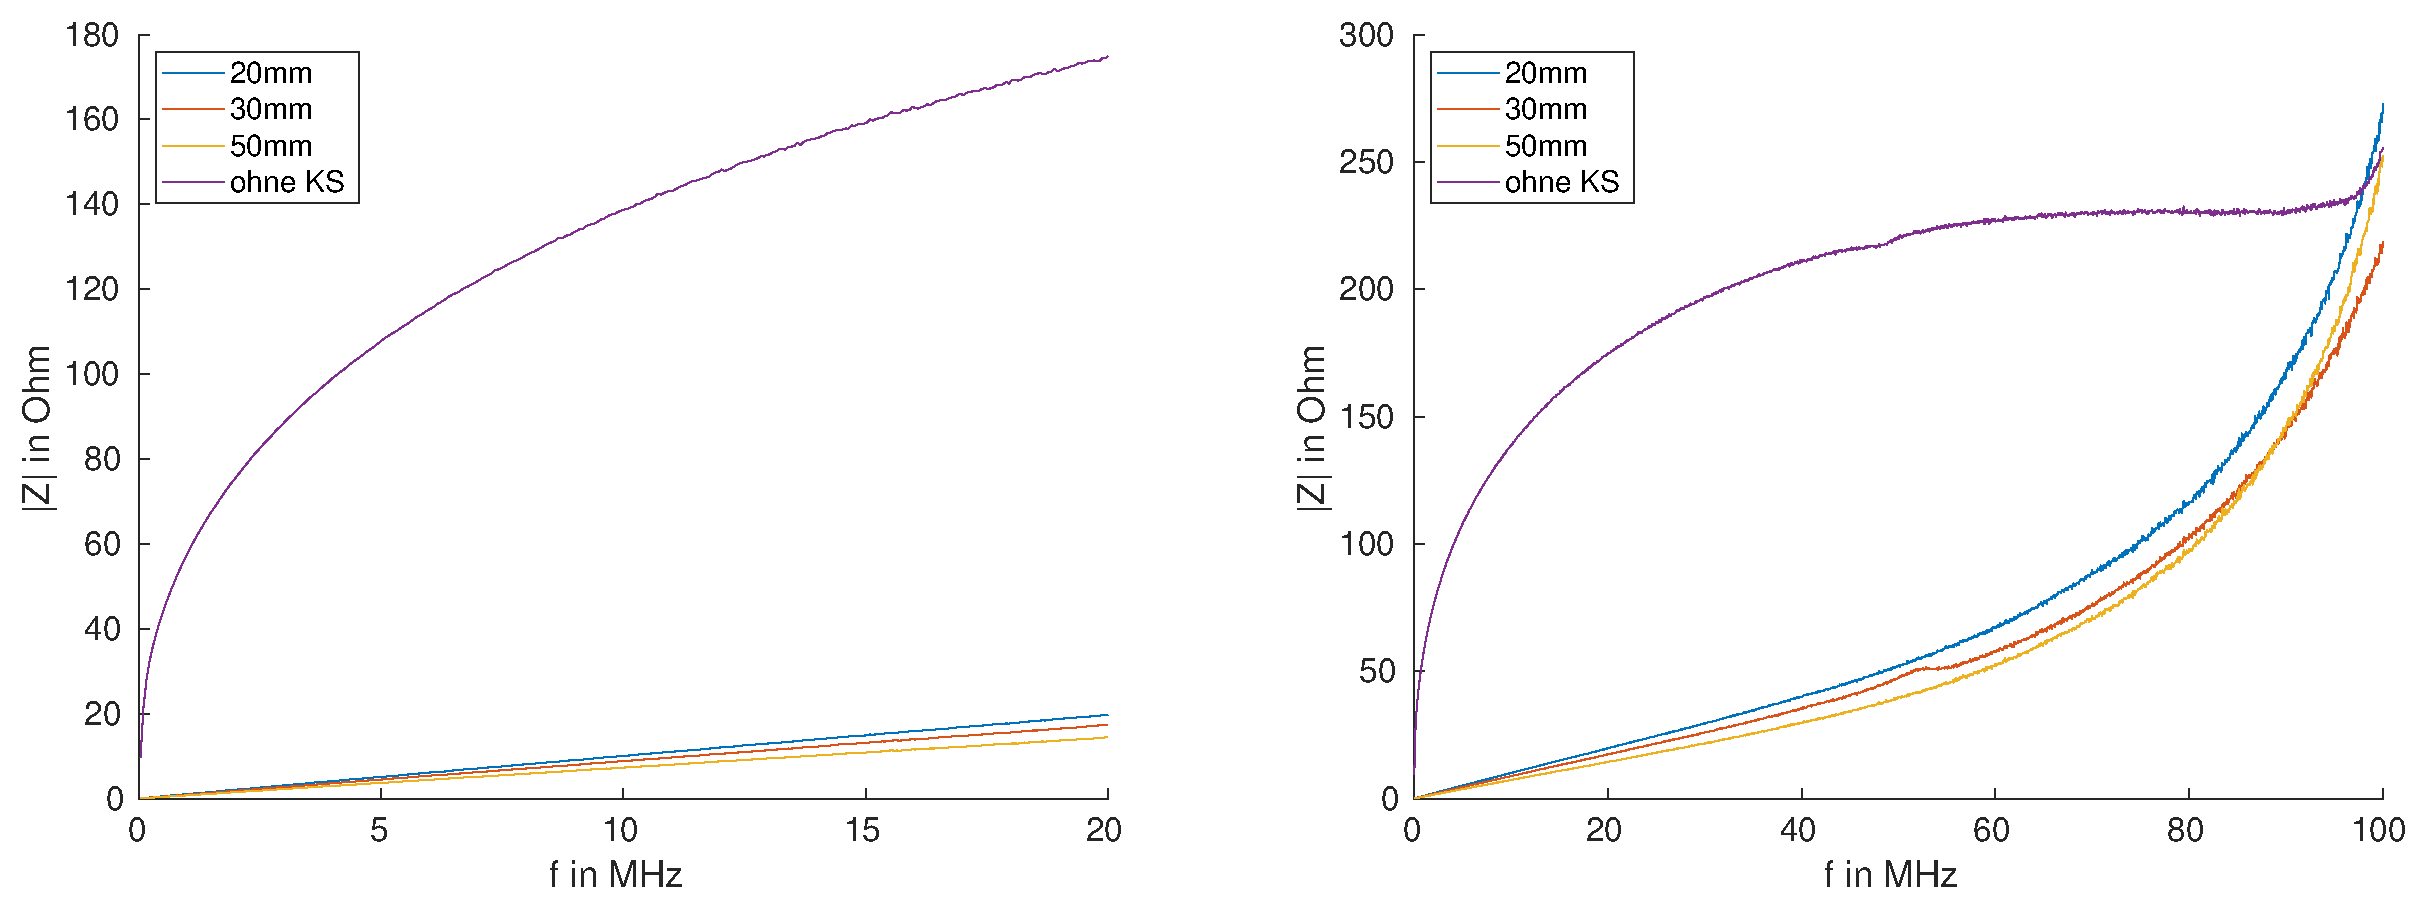
\includegraphics[width=\textwidth]{Z_RK_width_2KS}}
	\caption{Gegen\"uberstellung der Ringkernimpedanz f\"ur verschiedene Breiten der Kurzschl\"usse.}
	\label{fig:ringcorewidth}
\end{figure}

Auch hier wird wieder ein genaueres Augenmerk auf den relevanten Frequenzbereich unterhalb von $\SI{20}{\mega\hertz}$ gelegt. Dazu wird die Impedanz wieder bei den Frequenzen 5, 10 und $\SI{20}{\mega\hertz}$ dargestellt und die verschiedenen Breiten gegen\"ubergestellt. Dies ist in Abbildung~\ref{fig:ringcorewidth20} gezeigt.



\newpage



\begin{figure}[h]
	\centering
	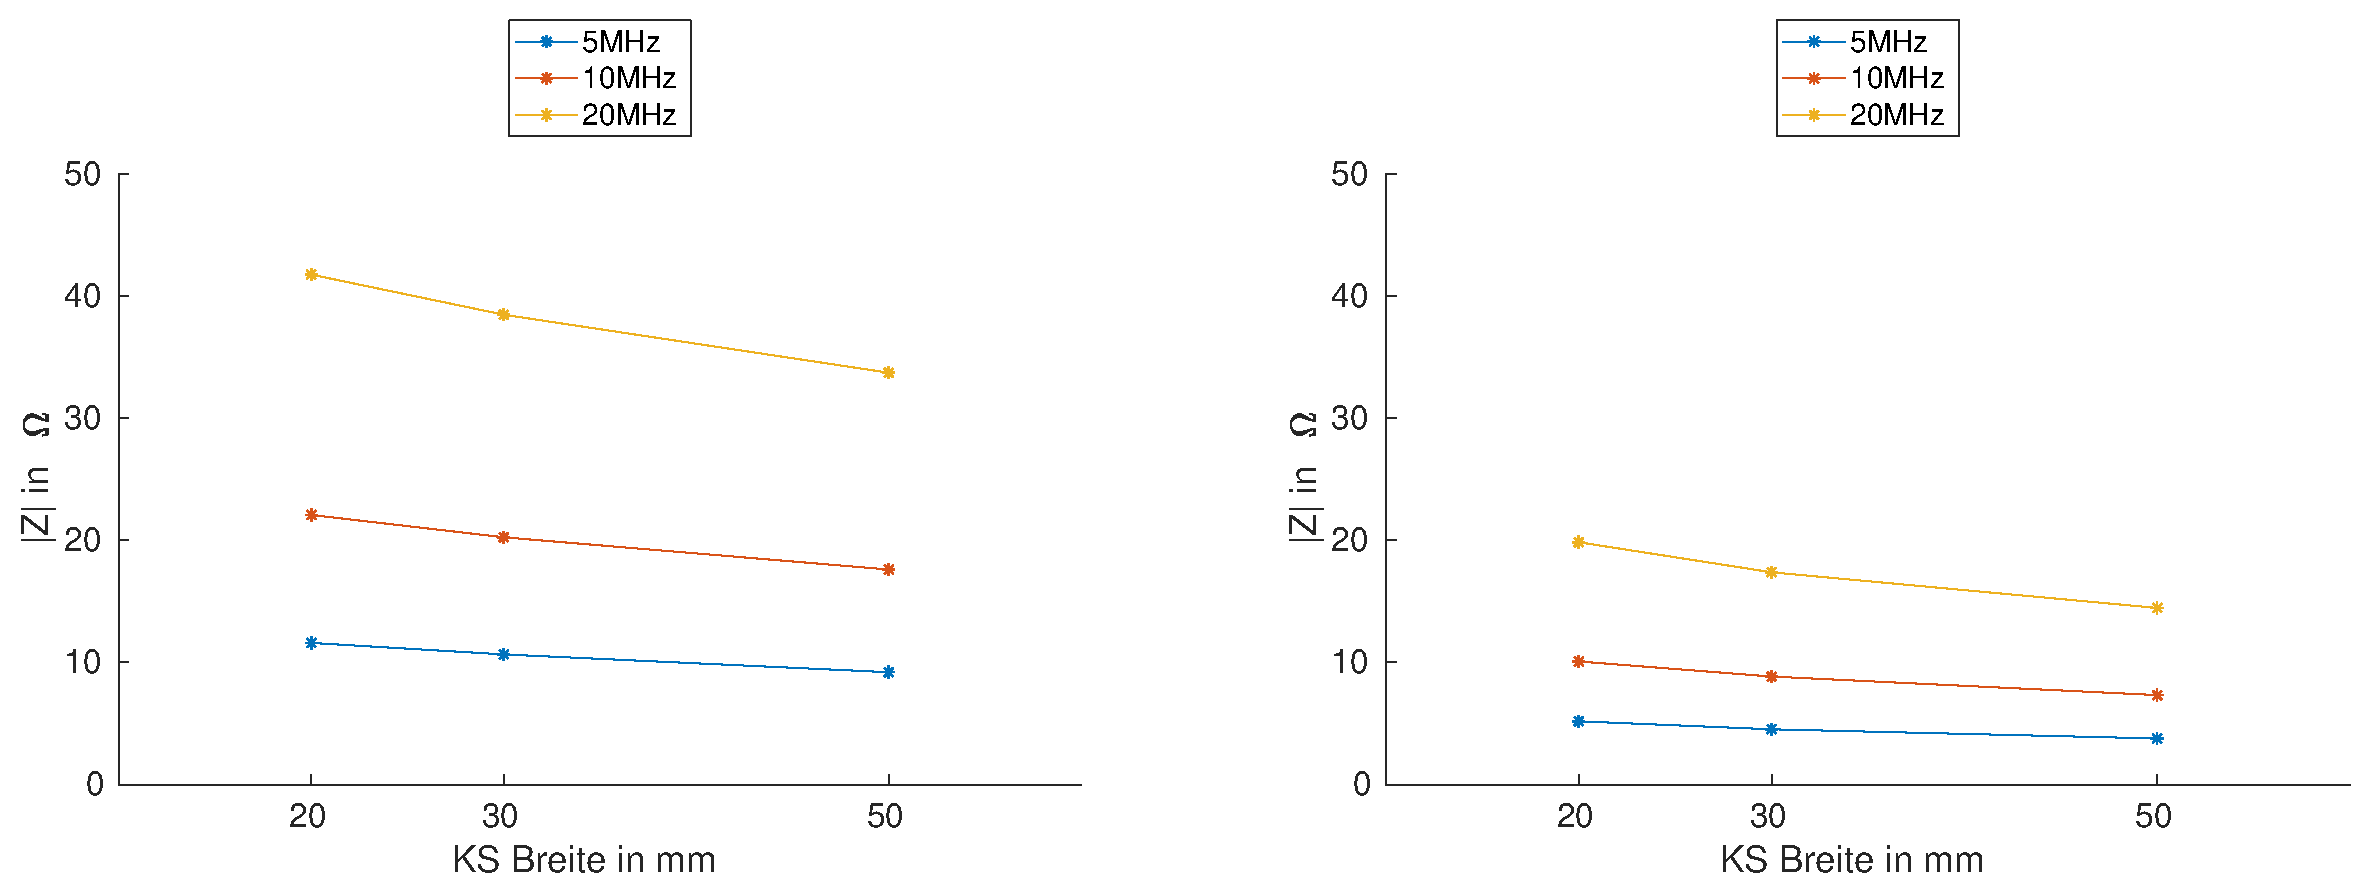
\includegraphics[width=\textwidth]{RK_Impedanz_width_frequenz}
	\caption{Gegen\"uberstellung der Ringkernimpedanz bei 5, 10 und $\SI{20}{\mega\hertz}$. Links: 1KS, rechts: 2KS.}
	\label{fig:ringcorewidth20}
\end{figure}

Das Ergebnis zeigt, dass ein breiterer Kurzschluss das Ergebnis der resultierenden Ringkernimpedanz weiter verringert. Diese Variation liefert im Extremfall, also dem Unterschied von $\SI{20}{\milli\meter}$ zu $\SI{50}{\milli\meter}$ bei einer Anzahl von zwei Kurzschl\"ussen und einer Frequenz von $\SI{20}{\mega\hertz}$, eine Verringerung der Ringkernimpedanz von rund $\SI{2,8}{\%}$. Dies zeigt, dass die Breite der Kurzschl\"usse eine geringere Auswirkung auf die resultierende Ringkernimpedanz hat, als die Anzahl der Kurzschl\"ussen. Besonders deutlich wird das im Vergleich zwischen einem Kurzschluss der Breite $\SI{50}{\milli\meter}$ mit zwei Kurzschl\"ussen der Breite $\SI{20}{\milli\meter}$ (siehe Anhang~\ref{anhang:Anordnung}). Trotz des geringeren Platzbedarfs, liefern die zwei schmalen Kurzschl\"usse eine deutlich geringere Impedanz.

\subsection{L\"ange der Kurzschl\"usse}
\"Ahnlich wie die Breite ist auch die L\"ange der Kurzschl\"usse problemlos zu varrieren. Hierbei ist allerdings darauf zu achten, dass die Kurzschlussb\"ugel mit Erh\"ohung der L\"ange auch n\"aher an den Rand der Testbox, beziehungsweise der Kavit\"at heran ragen. Die getesteten verschiedenen L\"angen sind in Abbildung~\ref{fig:ringcoreheightCST} gezeigt.

\begin{figure}[htb]
	\centering
	\subfloat[$\SI{160}{\milli\meter}$]{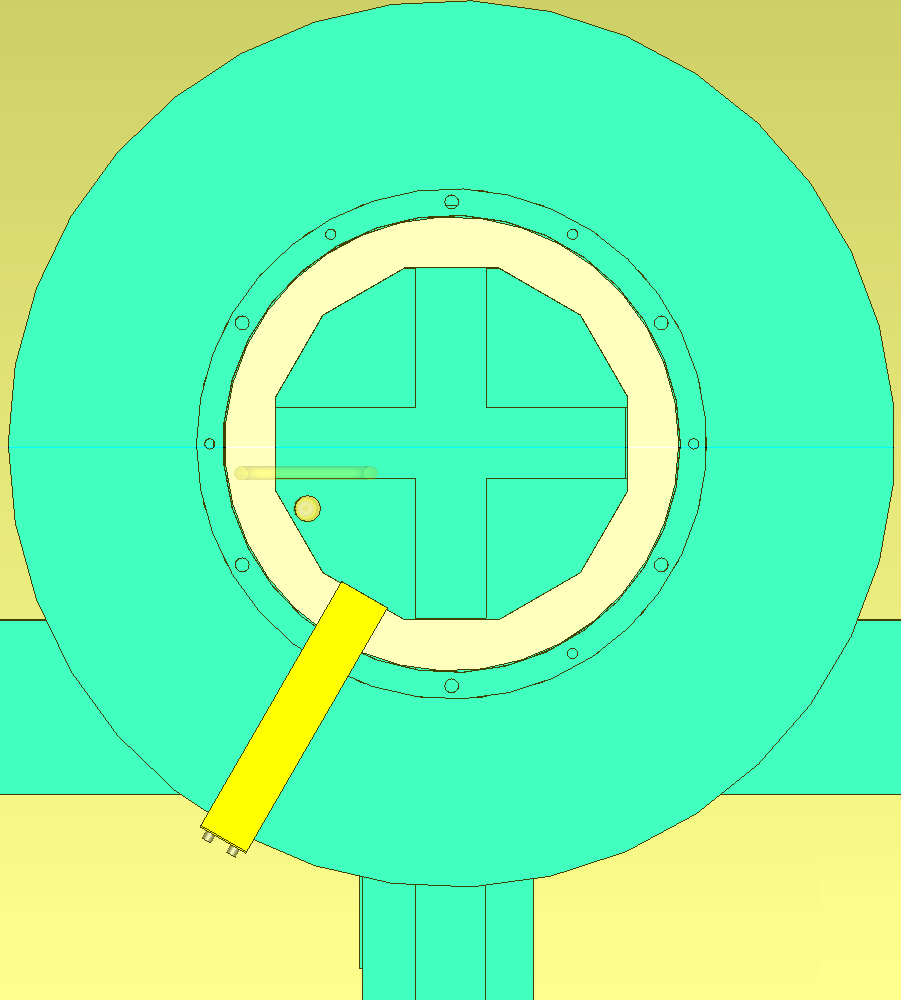
\includegraphics[height=0.3\textwidth]{1ksh160}}
	\hspace{0.05\textwidth}
	\subfloat[$\SI{200}{\milli\meter}$]{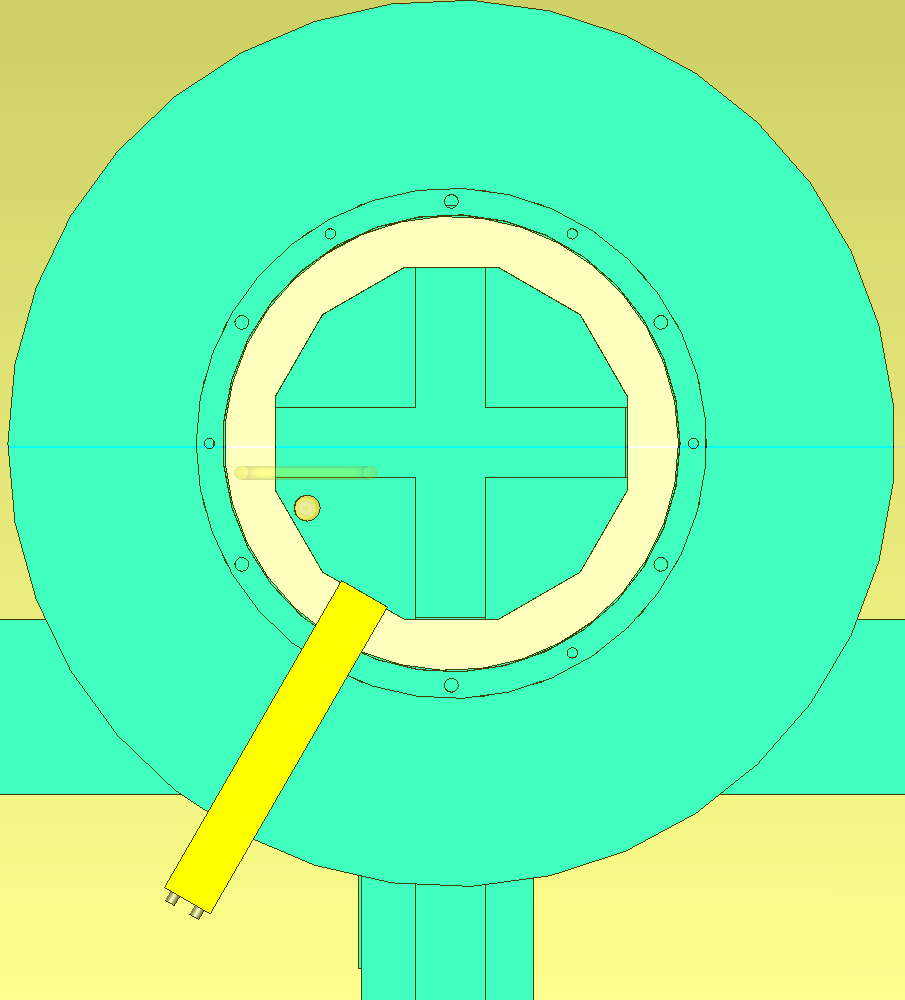
\includegraphics[height=0.3\textwidth]{1ksh200}}
	\hspace{0.05\textwidth}
	\subfloat[$\SI{250}{\milli\meter}$]{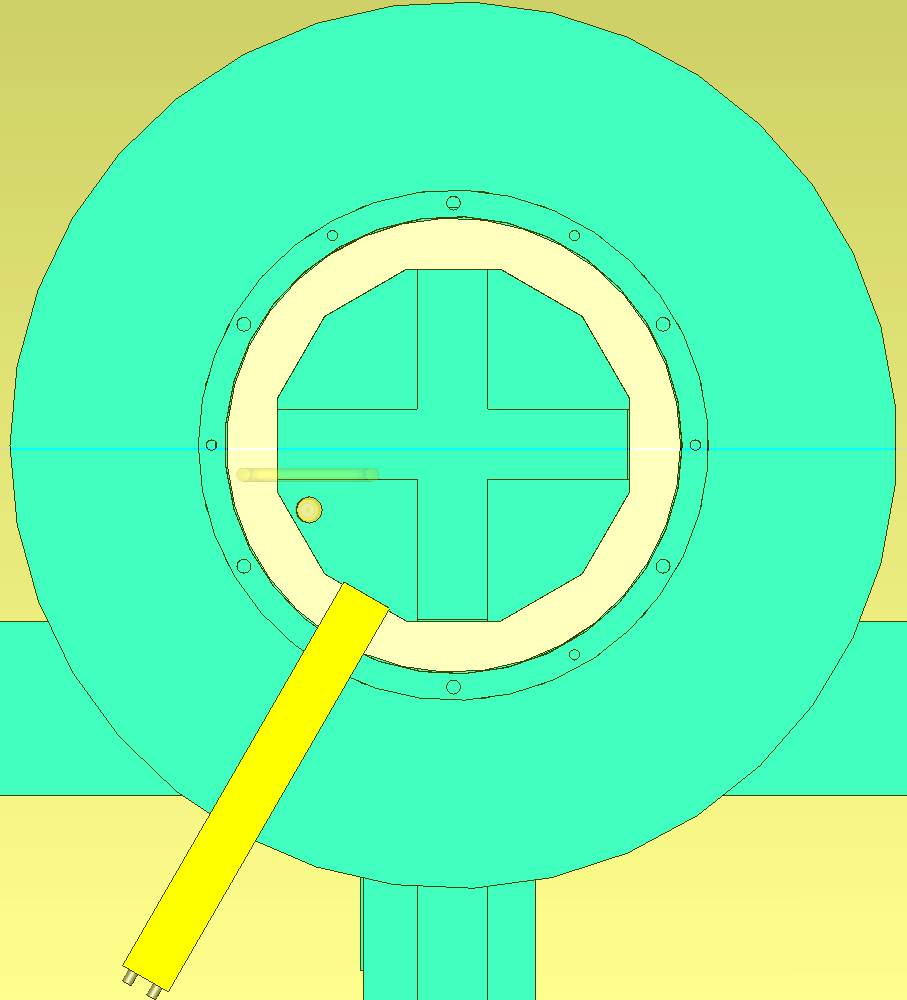
\includegraphics[height=0.3\textwidth]{1ksh250}}
	\caption{Jeweils ein montierter Kurzschluss mit verschiedenen L\"angen.}
	\label{fig:ringcoreheightCST}
\end{figure}

Die L\"ange der Kurzschl\"usse wird nach dem bekannten Vorgehen analysiert. Zun\"achst wird die Ringkernimpedanz \"uber der Frequenz nach Abbildung~\ref{fig:ringcoreheight} aufgetragen.

\begin{figure}[htb]
	\centering
	\subfloat[1 Kurzschluss]{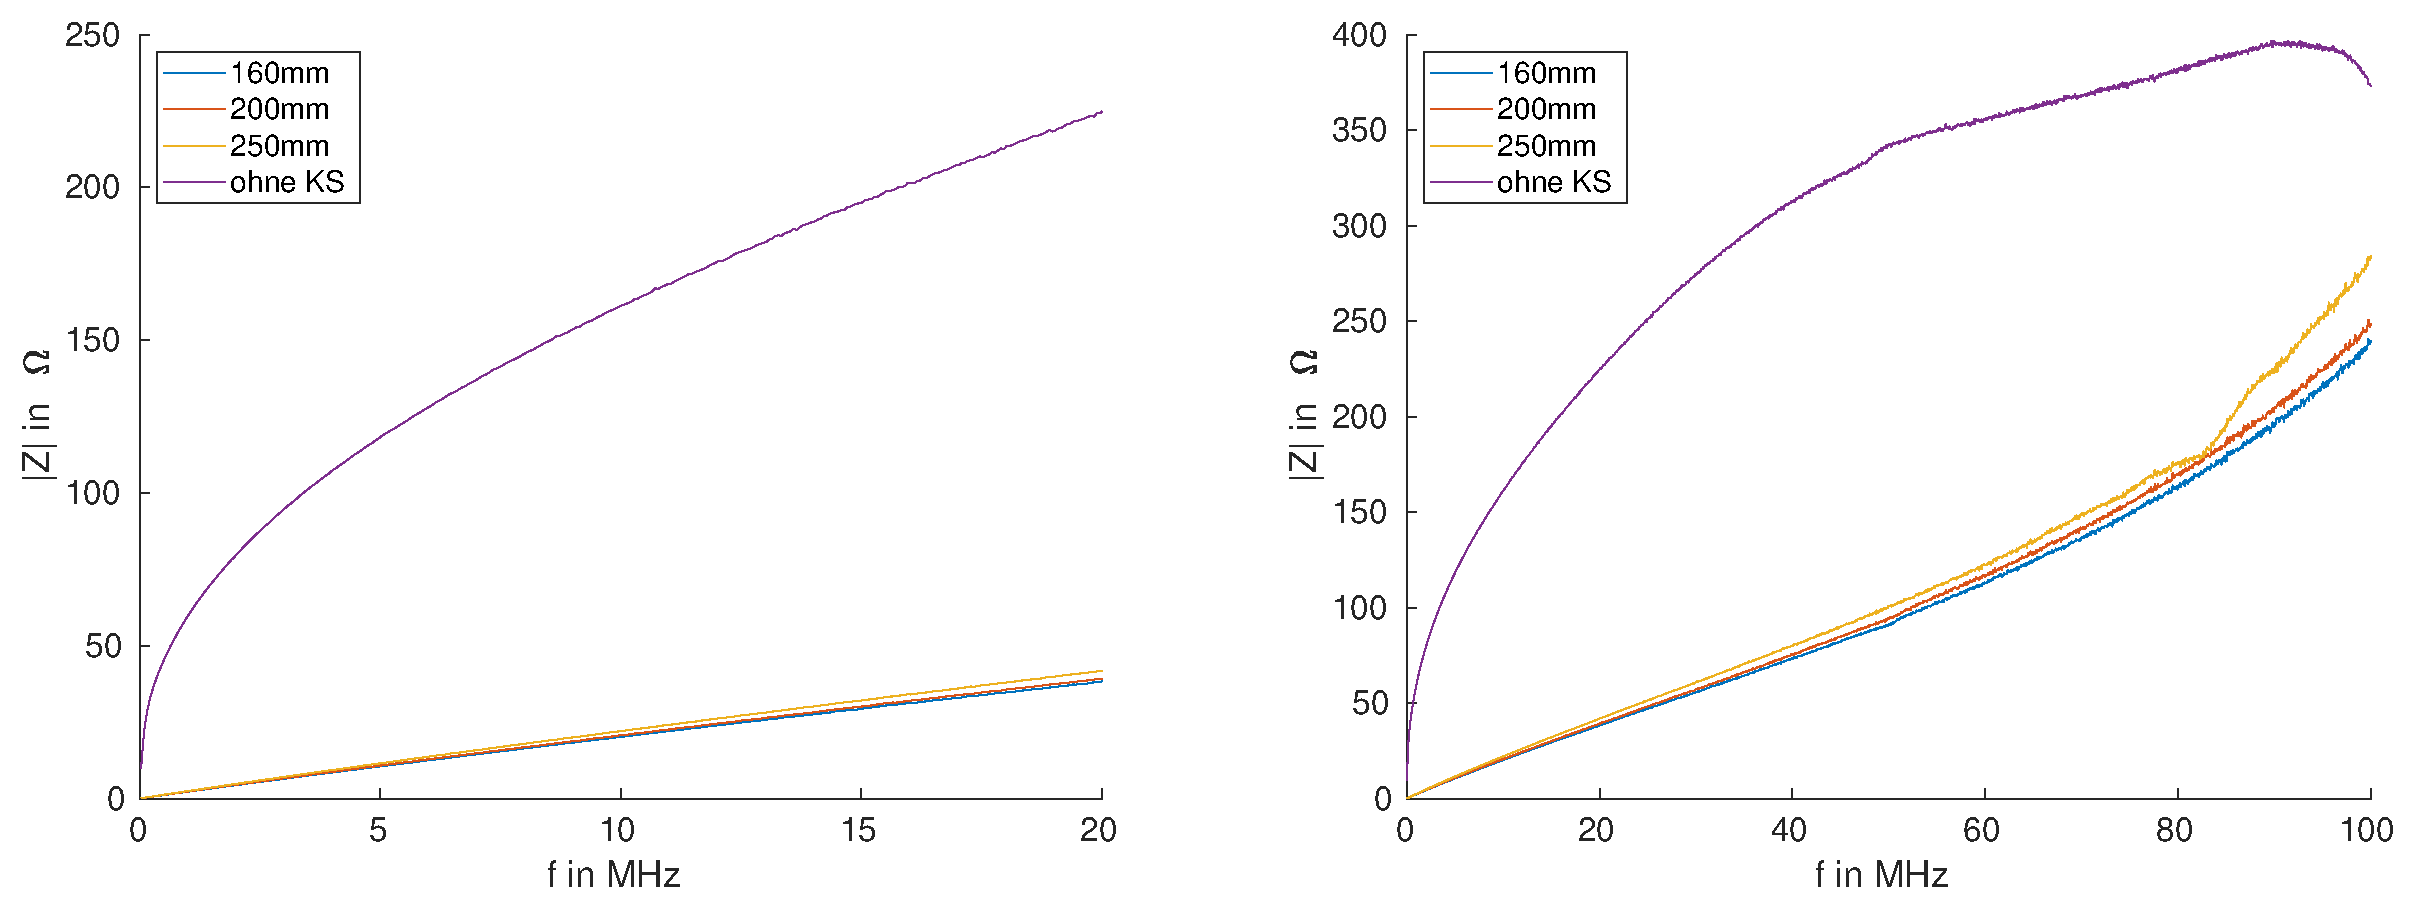
\includegraphics[width=\textwidth]{Z_RK_length_1KS}}
	\\
	\subfloat[2 Kurzschl\"usse]{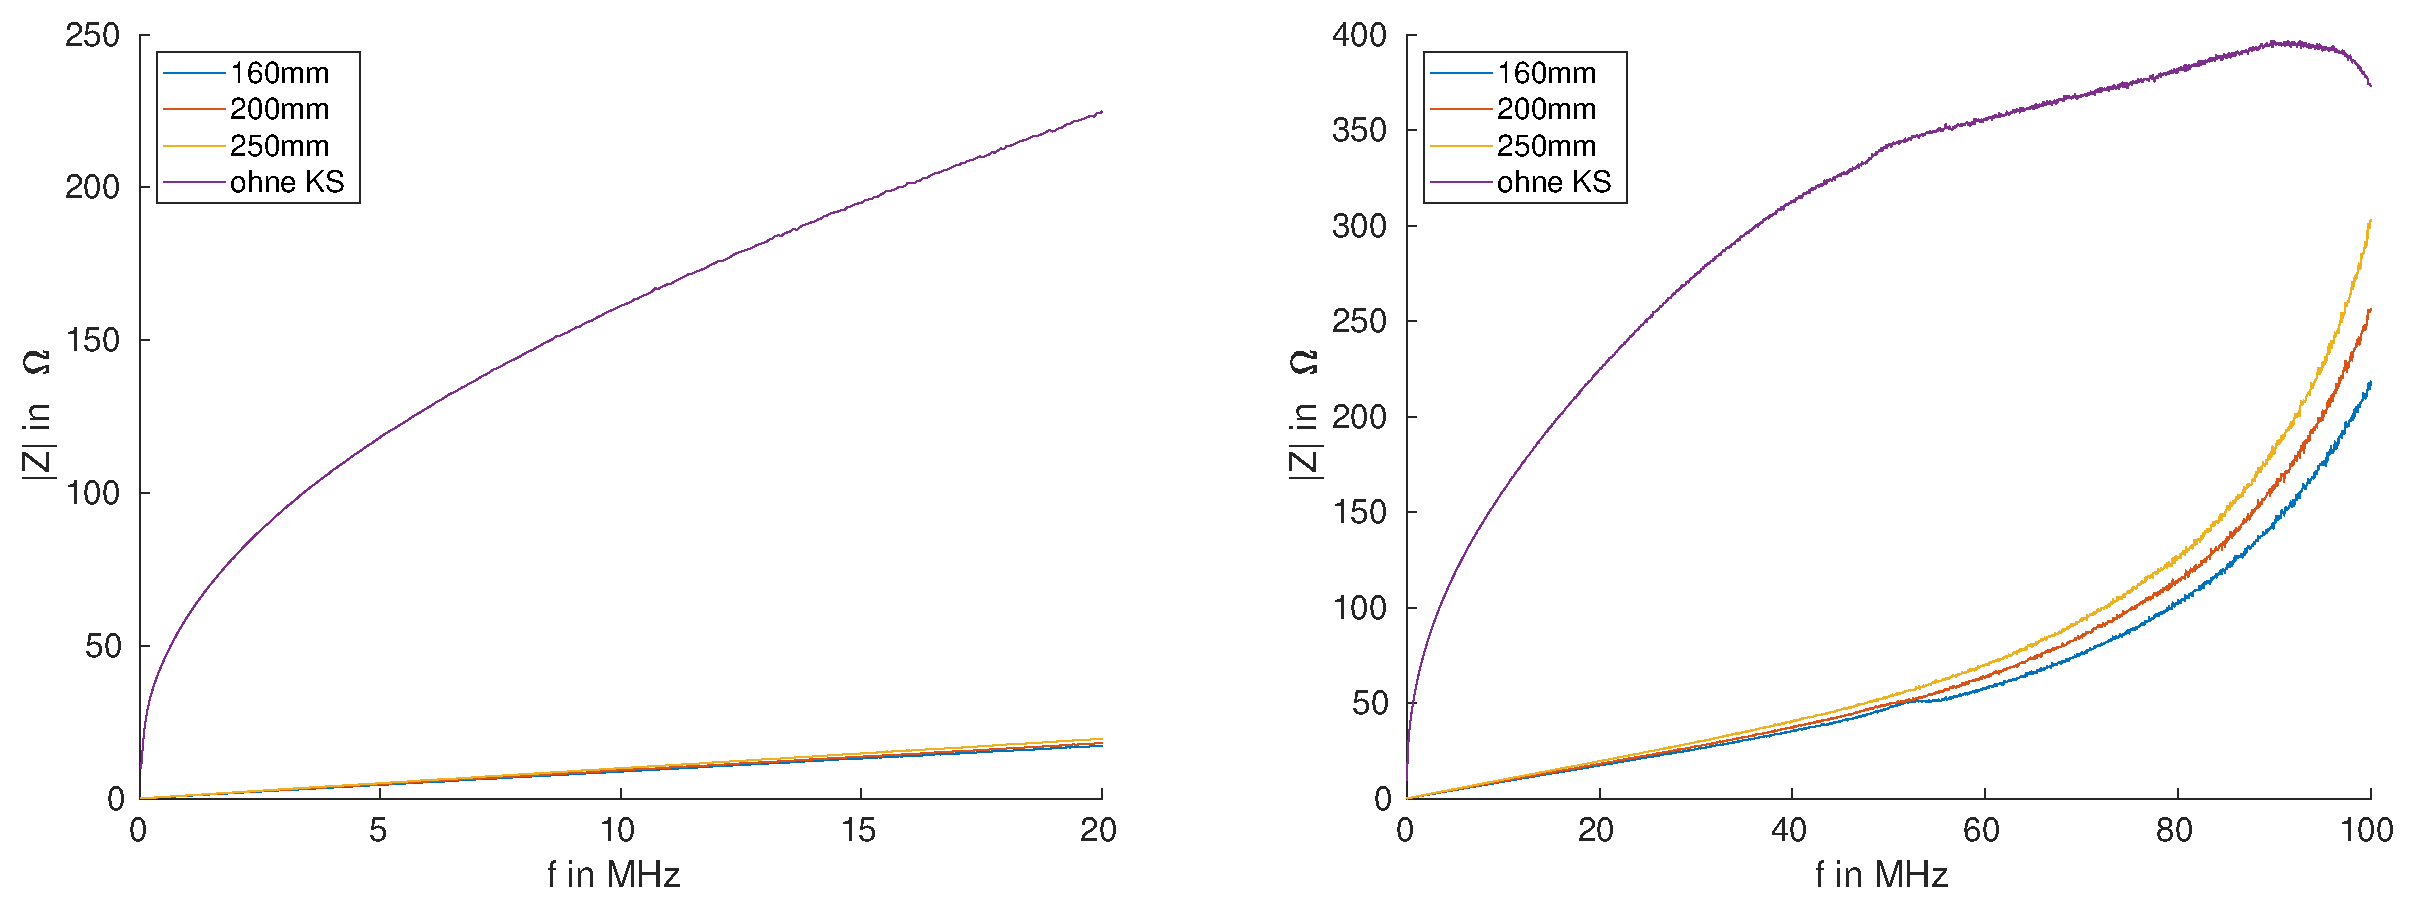
\includegraphics[width=\textwidth]{Z_RK_length_2KS}}
	\caption{Gegen\"uberstellung der Ringkernimpedanz f\"ur verschiedene L\"angen der Kurzschl\"usse.}
	\label{fig:ringcoreheight}
\end{figure}

Es f\"allt auf, dass der Effekt von l\"angeren Kurzschl\"ussen besonders im unteren Frequenzbereich noch deutlich geringer ausf\"allt, als es bei der Breitenvariation der Fall ist. Um das genauer Quantifizieren zu k\"onnen werden auch hier f\"ur Frequenzen von 5, 10 und $\SI{20}{\mega\hertz}$ die Ringkernimpedanz \"uber der L\"ange der Kurzschl\"usse aufgetragen. Das Ergebnis ist in Abbildung~\ref{fig:ringcoreheight20} zu sehen.




\newpage



\begin{figure}[htb]
	\centering
	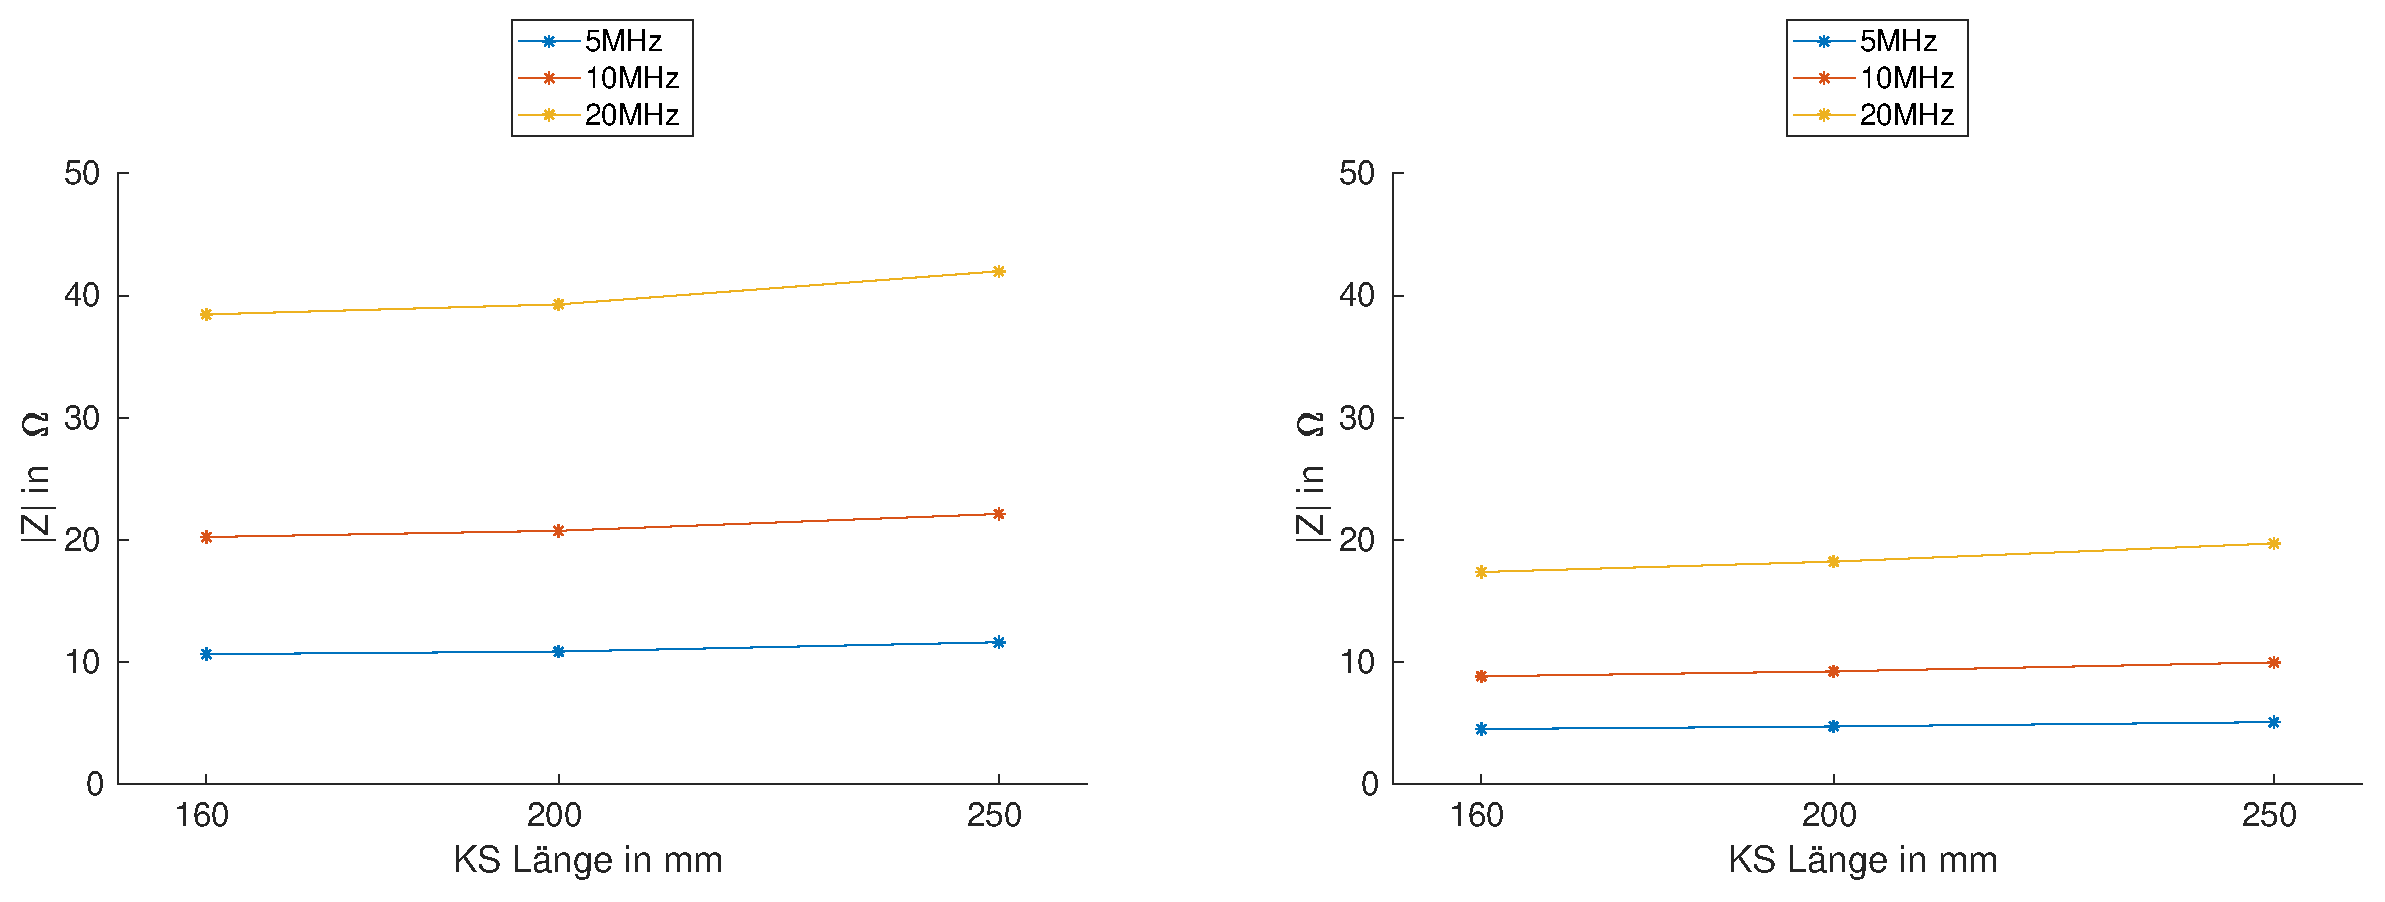
\includegraphics[width=\textwidth]{RK_Impedanz_length_frequenz}
	\caption{Gegen\"uberstellung der Ringkernimpedanz bei 5, 10 und $\SI{20}{\mega\hertz}$. Links: 1KS, rechts: 2KS.}
	\label{fig:ringcoreheight20}
\end{figure}

Der Extremfall ist hier die Variation bei $\SI{20}{\mega\hertz}$ und zwei Kurzschl\"ussen zwischen $\SI{160}{\milli\meter}$ und $\SI{250}{\milli\meter}$ L\"ange. Setzt man die Werte in Gleichung~\ref{eq:maxdiffpercent} ein, so erh\"alt man eine Abweichung von rund $\SI{1,3}{\%}$. 

\subsection{Dicke der Kurzschl\"usse}
Die Variation der Dicke ist in der Fertigung etwas aufwendiger. Zun\"achst m\"ussen die B\"ugel aus einem anderen Blech geschnitten werden. insbesondere das Biegen der B\"ugel gestaltet sich hierbei aber schwierig, da die zunehmende Dicke der Bleche das Biegen erschweren und h\"ohere Dicken anderes Werkzeug erforderten. Daher ist dieser Variationsparameter nur f\"ur zwei Dicken, n\"amlich $\SI{1}{\milli\meter}$ und $\SI{2}{\milli\meter}$ vorgesehen worden.
\par
Die Auftragung der Ringkernimpedanz \"uber der Frequenz liefert das in Abbildung~\ref{fig:ringcorethick} gezeigte Ergebnis.



\newpage




\begin{figure}[htb]
	\centering
	\subfloat[1 Kurzschluss]{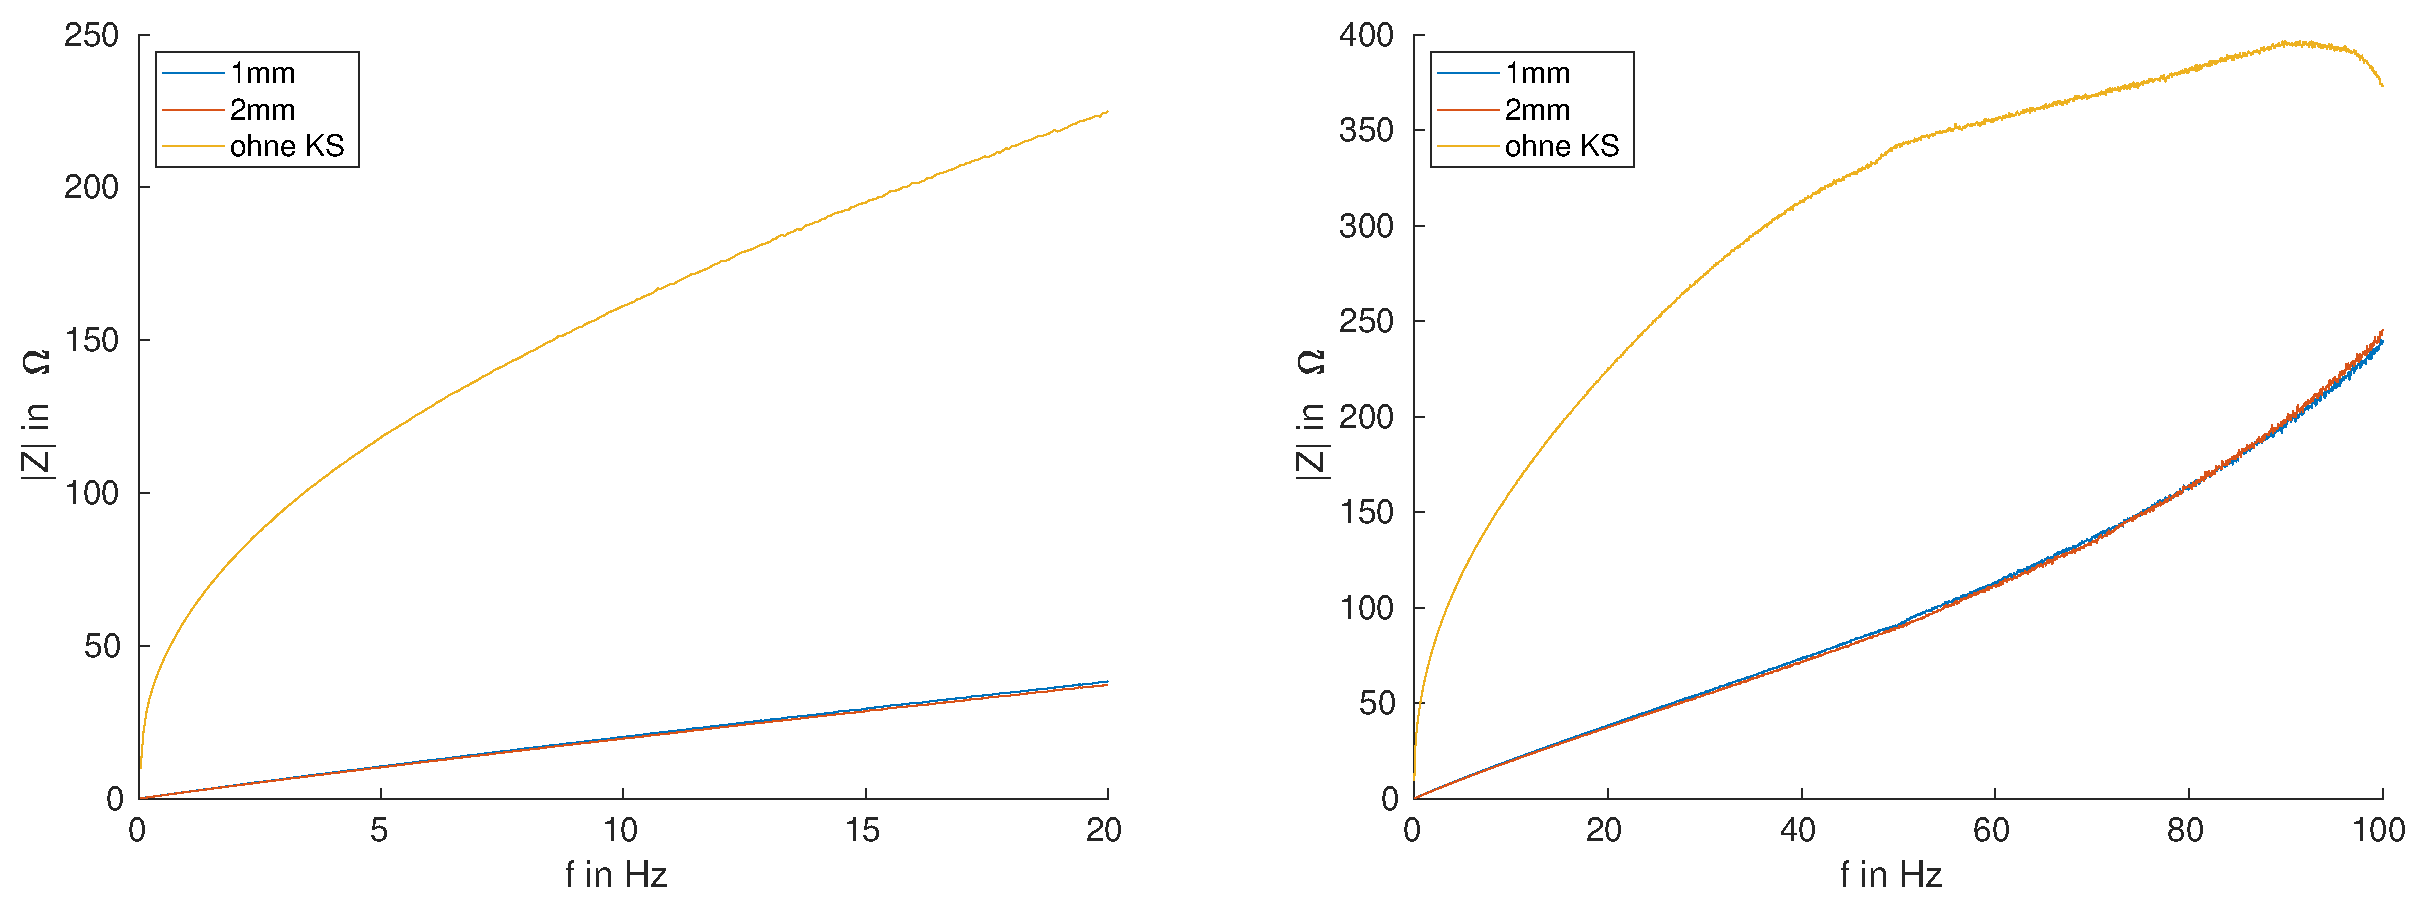
\includegraphics[width=\textwidth]{Z_RK_thick_1KS}}
	\\
	\subfloat[2 Kurzschl\"usse]{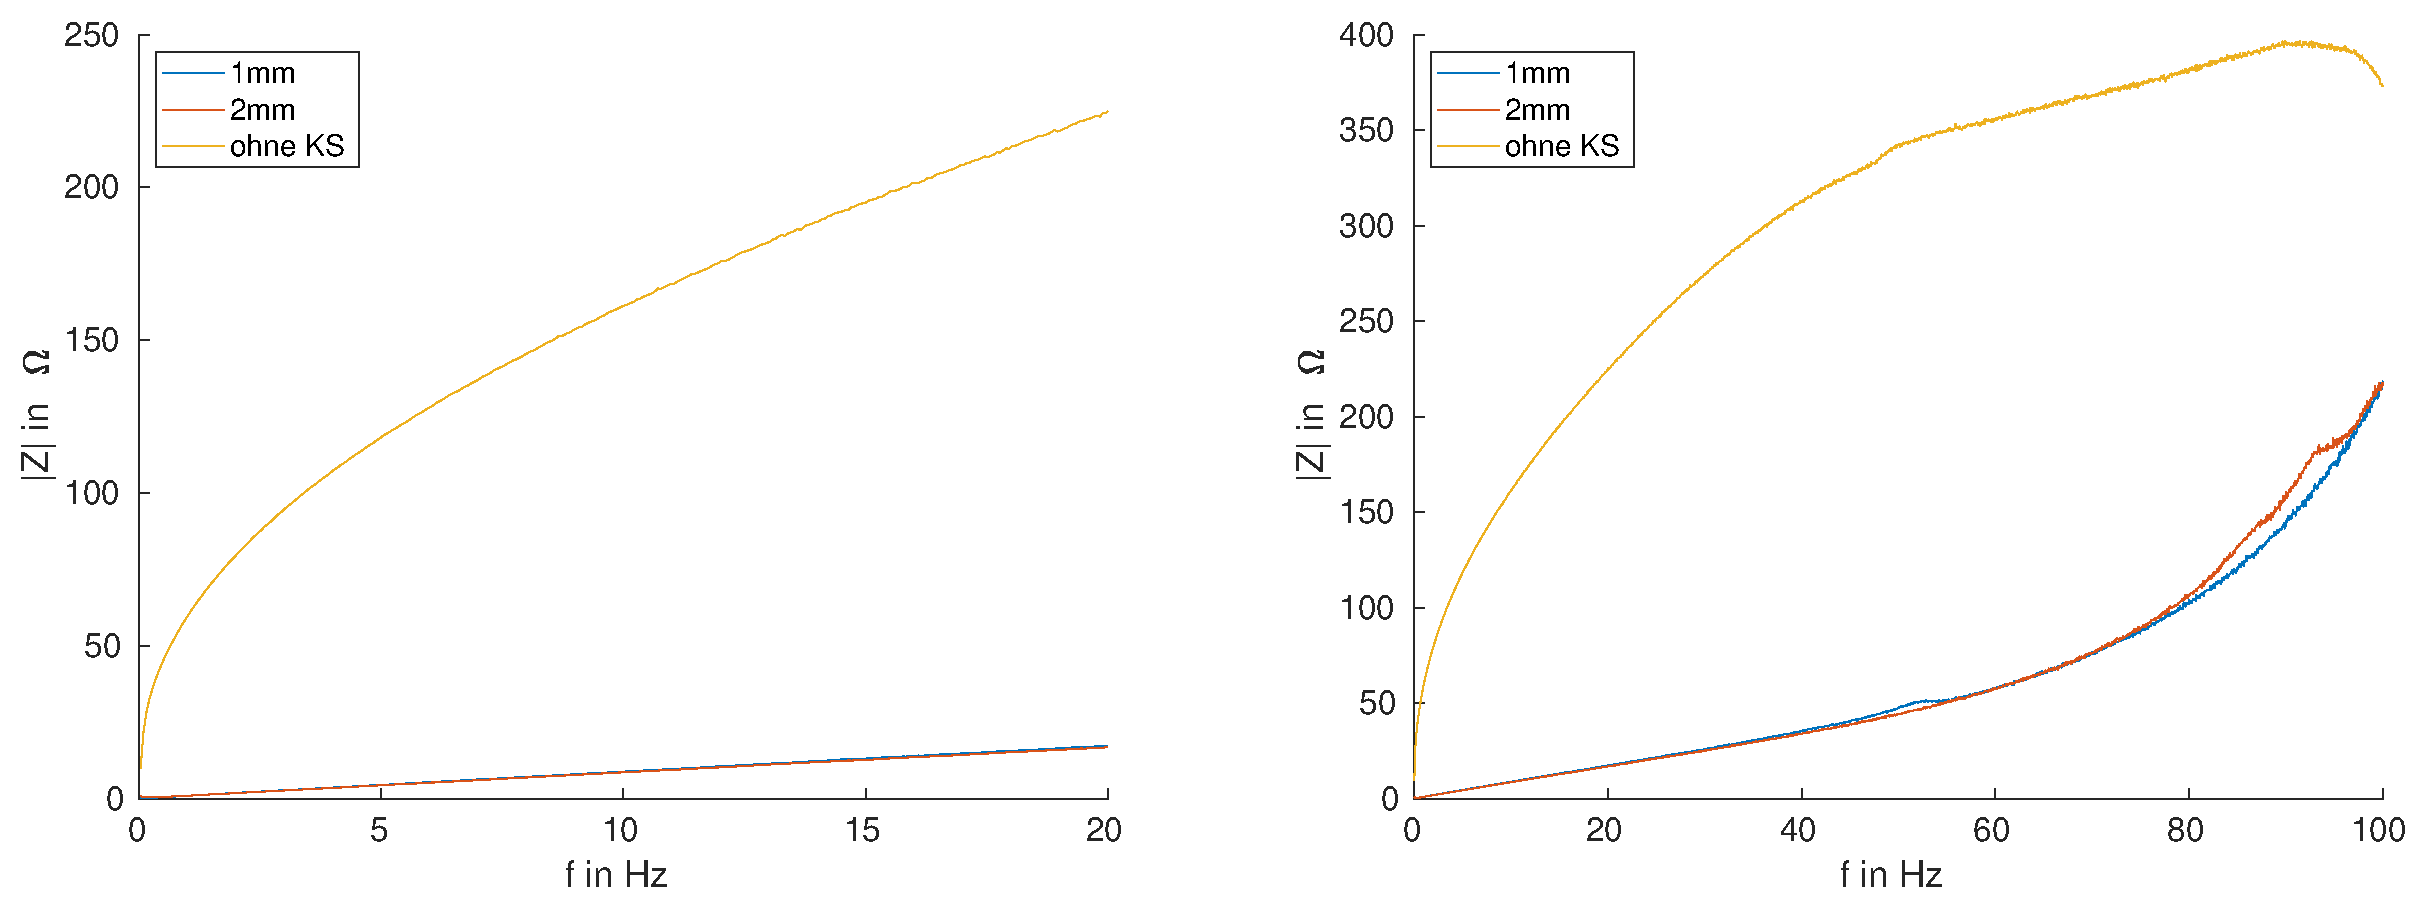
\includegraphics[width=\textwidth]{Z_RK_thick_2KS}} 
	\caption{Gegen\"uberstellung der Ringkernimpedanz f\"ur verschiedene Dicken der Kurzschl\"usse.}
	\label{fig:ringcorethick}
\end{figure}

Da nur zwei Stufen f\"ur die Dicke gemessen wurden, wird in diesem Fall auf eine Grafik f\"ur die einzelnen Frequenzpunkte verzichtet. Die Berechnung der Abweichung f\"ur den Vergleich von zwei Kurzschl\"ussen bei $\SI{20}{\mega\hertz}$ mit verschiedenen Dicken liefert nach Gleichung~\ref{eq:maxdiffpercent} einen prozentualen Wert von $\SI{0,286}{\%}$. 
Die Dicke des Blechs hat damit nahezu keinen Einfluss auf die Ringkernimpedanz.



\newpage
	\section{Einfluss im Leerlauf befindlicher Schienen auf die Ringkernimpedanz}
Es sollte nicht au\ss{}er acht gelassen werden, vorab montierte Kurzschlussschienen in der Testbox oder der Kavit\"at im laufenden Betrieb nicht einfach wieder entfernt werden k\"onnen. Es stellt sich die Frage, ob diese auch eine Auswirkung auf die Ringkernimpedanz haben, wenn sie nicht kurzgeschlossen sind. Im folgenden Abschnitt soll daher analysiert werden, ob auch Schienen, welche sich im Leerlauf befinden, einen Einfluss auf die Impedanz haben k\"onnen.
	\section{Feldbilder}
Um eine weitgehendere Analyse der Auswirkung von Kurzschl\"ussen zu f\"uhren, k\"onnen aus CST Feldbilder ausgelesen werden. Diese zeigen, in wie weit das magnetische Feld durch die Kurzschl\"usse aus dem inneren des MA-Ringkerns verdr\"angt wird. Dazu werden einige Kurzschlussanordnungen gegen\"uber gestellt. Zun\"achst wird der Einfluss eines einzigen Kurzschlusses mit der Breite $\SI{30}{\milli\meter}$, der Länge $\SI{160}{\milli\meter}$ sowie einer Blechdicke von $\SI{1}{\milli\meter}$ gegen\"uber dem reinen Ringkern ohne Kurzschl\"usse nach Abbildung~\ref{fig:0zu1ks} betrachtet.


\newpage



\begin{figure}[htb]
	\centering
	\subfloat[Ringkern ohne Kurzschl\"usse]{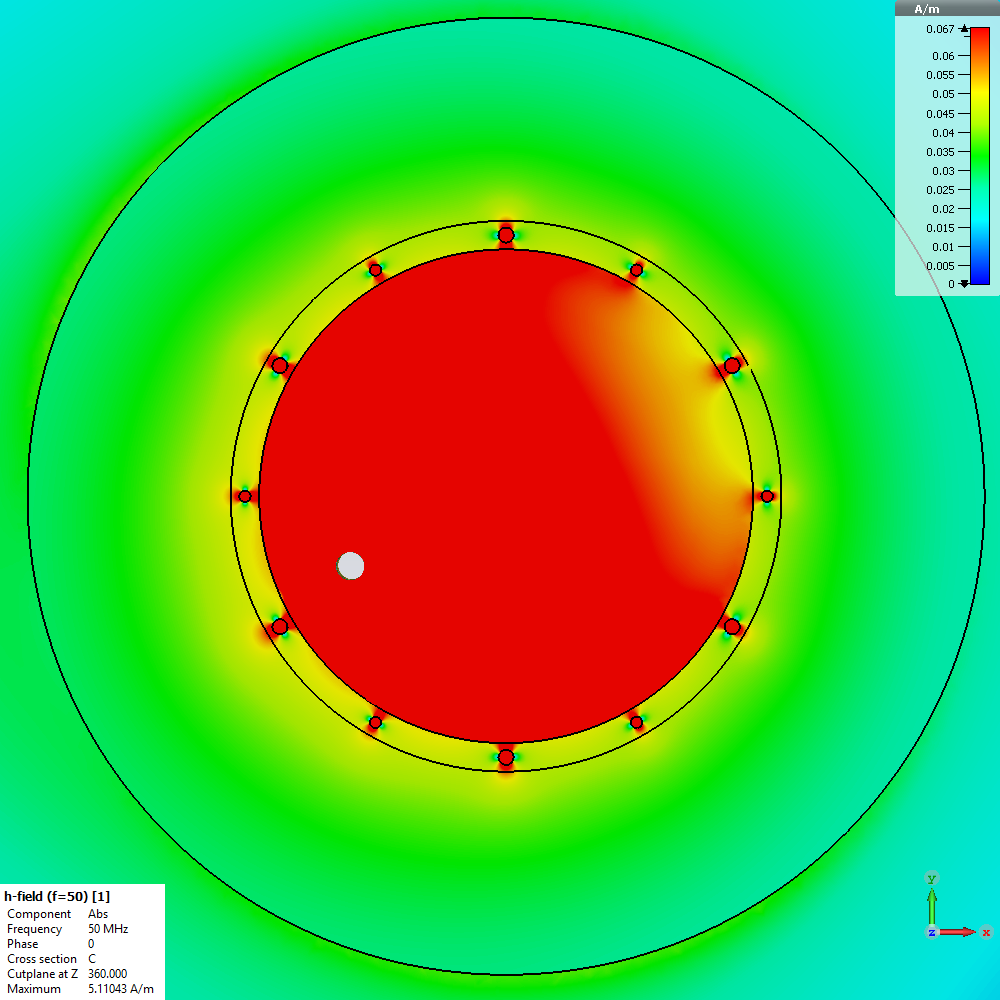
\includegraphics[height=0.42\textwidth]{Feldbilder/0KS}}
	\subfloat[Ringkern mit einem Kurzschluss der Breite $\SI{30}{\milli\meter}$ und der Länge $\SI{160}{\milli\meter}$.]{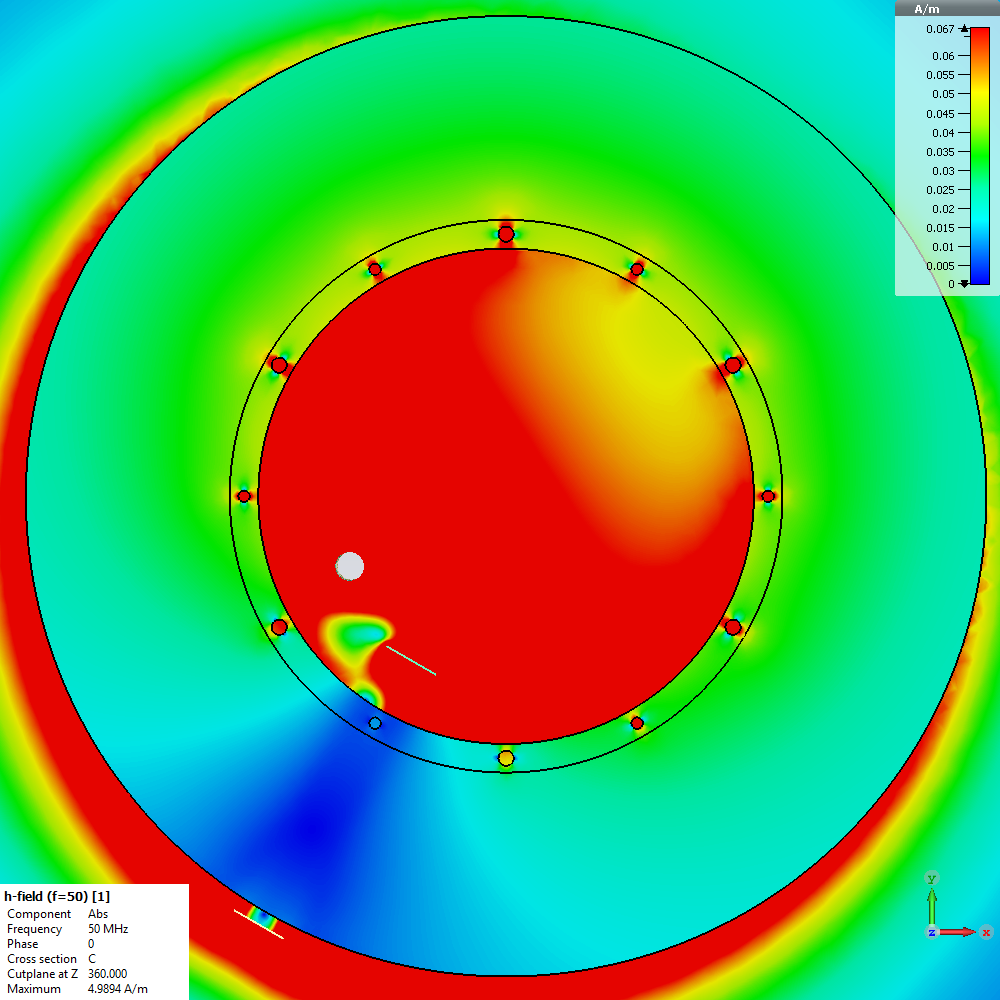
\includegraphics[height=0.42\textwidth]{Feldbilder/1KS}}
	\subfloat[Legende]{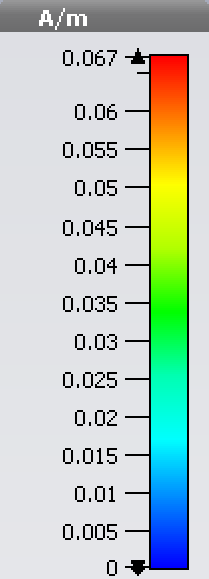
\includegraphics[height=0.42\textwidth]{Feldbilder/legend}}
	\caption{Gegen\"uberstellung der Feldverteilung des Magnetischen Feldes innerhalb des Ringkerns ohne Kurzschluss und mit einem Kurzschluss.}
	\label{fig:0zu1ks}
\end{figure}
\par
Bereits ein Kurzschluss verd\"angt schon einen gro\ss{}en Teil des magnetischen Feldes. Dieser Effekt ist in dem Bereich des Ringkerns, welcher von der Kurzschlusschiene \"uberdeckt ist, oder in der N\"ahe liegt deutlich st\"arker als in anderen Ringkernregionen. Dieser Effekt ist auch bei einer h\"oheren Anzahl an Kurzschl\"ussen sichtbar. Abbildung~\ref{fig:1zu8ks} zeigt den Vergleich von einem Kurzschluss zur maximalen Anzahl von acht Kurzschl\"ussen.
\begin{figure}[htb]
	\centering
	\subfloat[Ringkern mit einem Kurzschluss der Breite $\SI{30}{\milli\meter}$ und der Länge $\SI{160}{\milli\meter}$.]{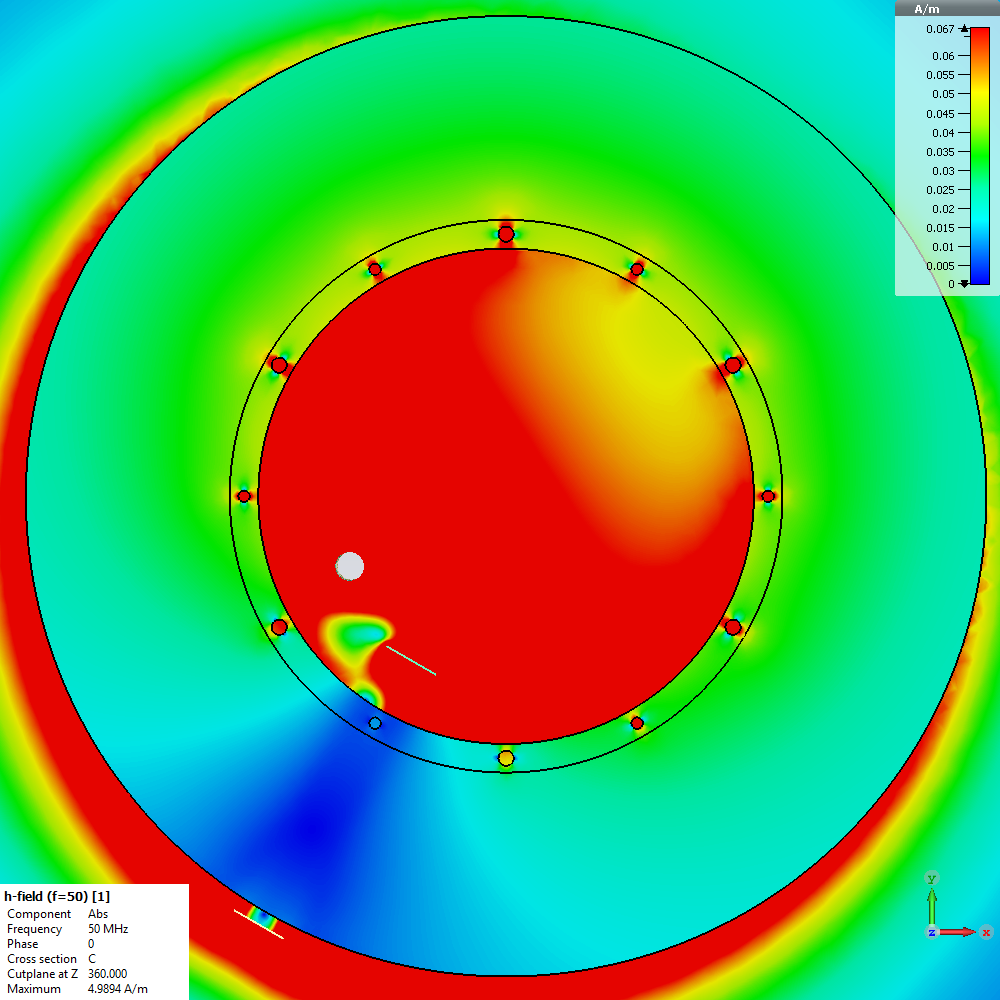
\includegraphics[height=0.42\textwidth]{Feldbilder/1KS}}
	\subfloat[Ringkern mit acht Kurzschl\"ussen der Breite $\SI{30}{\milli\meter}$ und der Länge $\SI{160}{\milli\meter}$.]{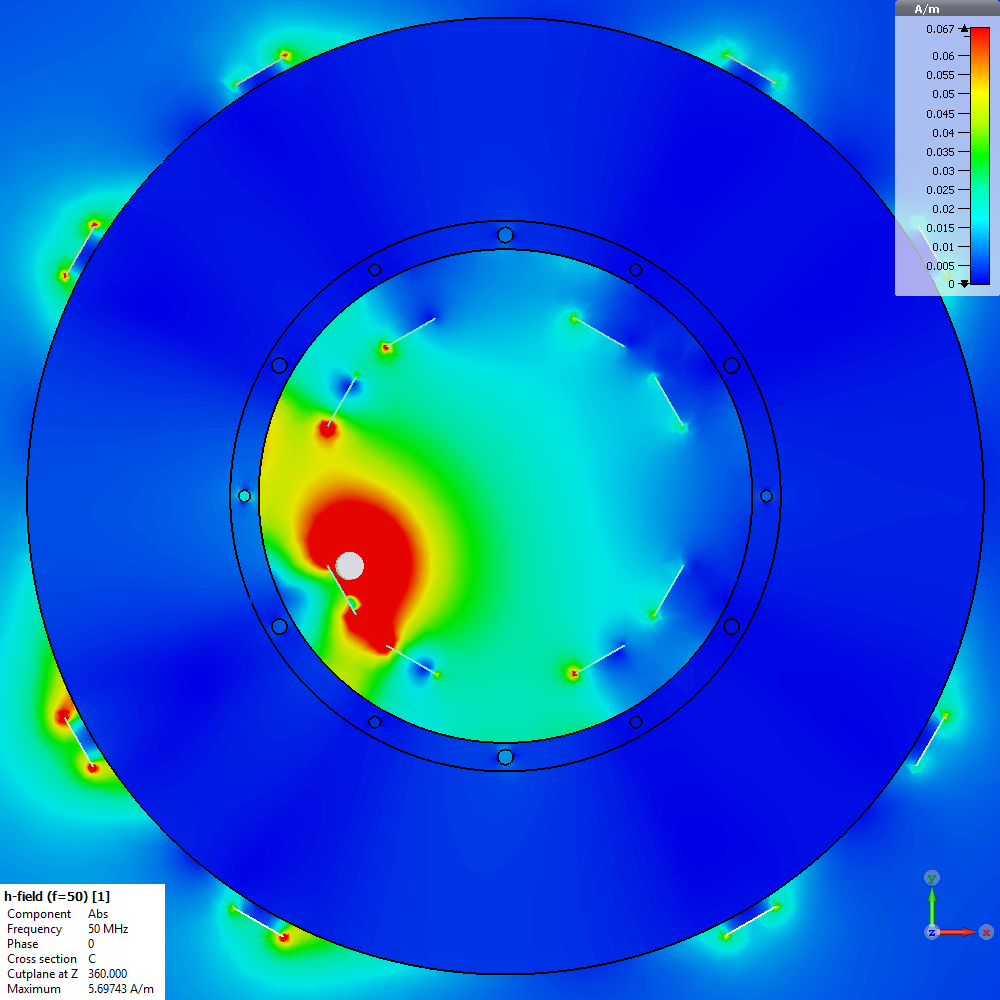
\includegraphics[height=0.42\textwidth]{Feldbilder/8KS}}
	\subfloat[Legende]{\includegraphics[height=0.42\textwidth]{Feldbilder/legend}}
	\caption{Gegen\"uberstellung der Feldverteilung des magnetischen Feldes innerhalb des Ringkerns mit einem Kurzschluss und mit acht Kurzschl\"ussen.}
	\label{fig:1zu8ks}
\end{figure}
\par
Die Beobachtung liefert auch eine Erkl\"arung, warum zwei schmale Kurzschl\"usse eine st\"arkere Verringerung der Ringkernimpedanz nach sich ziehen, als ein breiter Kurzschluss. Da das Feld besonders im Umkreis des Kurzschlusses geringer ist, f\"uhrt eine weitere Verteilung der Kurzschl\"usse zu geringeren Feldst\"arken im gesamten Ring. Dieser Effekt ist in Abbildung~\ref{fig:150zu220ks} zu sehen. 
\begin{figure}[htb]
	\centering
	\subfloat[Ringkern mit einem Kurzschluss der Breite $\SI{50}{\milli\meter}$ und der Länge $\SI{160}{\milli\meter}$.]{\includegraphics[height=0.42\textwidth]{Feldbilder/1KSb50}}
	\subfloat[Ringkern mit zwei Kurzschl\"ussen der Breite $\SI{20}{\milli\meter}$ und der Länge $\SI{160}{\milli\meter}$.]{\includegraphics[height=0.42\textwidth]{Feldbilder/2KSb20}}
	\subfloat[Legende]{\includegraphics[height=0.42\textwidth]{Feldbilder/legend}}
	\caption{Gegen\"uberstellung der Feldverteilung des magnetischen Feldes innerhalb des Ringkerns mit einem Kurzschluss der Breite $\SI{50}{\milli\meter}$ und mit zwei Kurzschl\"ussen der Breite $\SI{20}{\milli\meter}$.}
	\label{fig:150zu220ks}
\end{figure}
\par
Wird vorausgesetzt, dass die Ringkernimedanz direkt mit dem mittleren Feld zusammenh\"angt, so dient dies als eine plausible Erkl\"arung f\"ur bisher beobachtete Effekte. Die komplette Ansicht der Feldverteilung f\"ur alle Kurzschlussanordnungen ist in Anhang~\ref{sec:allfieldplots} gegeben.
	
\chapter{Fazit und Ergebnis}\label{chap:fazit}
	\section{Fazit}
was wurde gemacht:
\begin{itemize}
	\item Testbox vermessen
	\item Testbox modifiziert um reproduzierbar zu messen
	\item Messung durchgef\"uhrt, reproduzierbar
	\item Simulation angepasst, dass diese in geringer Abweichung f\"ur weitere Variationen genutzt werden kann
	\item Ergebnisse quantifiziert, evaluiert
\end{itemize}
was wurde beobachtet:
\begin{itemize}
    \item ein KS bringt schon eine Annullierung von ca. $80~\%$
    \item mit 7 KS fast kein Einfluss durch RK mehr
    \item Breite, Länge und Dicke haben vergleichbar geringen Einfluss
\end{itemize}
welche Schlüsse werden daraus gezogen:
\begin{itemize}
    \item je nach einbaumöglichkeit besser schmalere, kurze, nah um den RK und passende Anzahl wählen
\end{itemize}

\section{Ausblick}
\begin{itemize}
    \item verbesserung der Simulationsmodell mit besserer anpassung der materialparameter
    \item anpassung der parameter an die Umgebung der kavität
    
\end{itemize}

	
%% Appendix %%%%%%%%%%%%%%%%%%%%%%%%%%%%%%%%%%%%%%%%%%%%%%%%%%%%%%%%%%%%%%%%
\pagestyle{plain}
\appendix
\newcommand{\hiddensection}[1]{
    \stepcounter{section}
    \section*{\Alph{chapter}.\arabic{section}\hspace{0.8em}{#1}}
}
\chapter{Appendix: --}<<<
%    \input{../Inputfiles/Chapters/_.tex}


%%%%%%%%%%%%%%%%%%%%%%%%%%%%%%%%%%%%%%%%%%%%%%%%%%%%%%%%%%%%%%%%%%%%%%%%%%

\newpage
% {\Huge AB HIER WIP, NICHT IN DER ENDSTRUKTUR}
% 
% \newpage
    
% \chapter{Bearbeitung}
%     \section{Vorbereitung}
    \begin{enumerate}
        \item Zu untersuchende Parameter:
            \begin{enumerate}
                \item Anordnung des Kurzschlusses (in Relation zur Strahlführung, Abstand zum Ringkern, Anordnung um den Ringkern)
                \item Anzahl der Kurzschlüsse
                \item Form
                \item Abmessungen (Größe)
            \end{enumerate}
    \end{enumerate}
%     \section{Messung}
    \begin{enumerate}
        \item Messung der Impedanz mittels Network Analysers
        \item Messung verschiedener Aufbauten
            \begin{enumerate}
                \item leere Box (als Referenz)
                \item mit Ringkern
                \item verschiedene Arten und Anordnungen von Kurzschlüssen
            \end{enumerate}
    \end{enumerate}
%         \section{Motivation}
    Um die Einflüsse verschiedener Kurzschlussanordnungen und -ausführungen schon im Vorfeld abschätzen zu können und ein erstes Gefühl für den Einfluss der Kurzschlüsse zu bekommen, wurde die Testanordnung zunächst ausgiebig mit der Simulationssoftware CST simuliert.\\
    Die Simulationen dienten als Vorbereitung, um bei den Messungen präziser vorgehen zu können und gezielt Messungen durchzuführen. Zuletzt wurden die Simulationsergebnisse dann mit den Messergebnissen gegenübergestellt und verglichen, um deren Richtigkeit zu überprüfen.
    
    \section{Modellierung}
        \subsection{Bestehendes Testbox- und Ringkernmodell}
        Als Grundlage für die Simulation der Testbox und des Ringkerns dient das Simulationsmodell von Testbox inklusive Ringkern aus der Bachelorarbeit von Denys Bast \citep{bast2017ba}.\\
        Die Außenwände der Testbox sind geometrisch sehr genau den Abmessungen des realen Teststandes entsprechend modelliert, als Material wird hierfür reines Kupfer verwendet, wie es in der Datenbank von CST zu finden ist. Die leere Box ist in Abbildung~\ref{fig:BoxCST} dargestellt.
        
            \begin{figure}[htb]
                \centering
                \includegraphics[height=0.4\textwidth]{./Simulation/BoxWaende2.png}
                \caption{Modell der Testbox in CST}
                \label{fig:BoxCST}
            \end{figure}
        In Abbildung~\ref{fig:InnenleiterCST} ist die Signaleinkopplung der Testbox zu sehen.
        Diese ist als Hohlzylinder aus Kupfer modelliert und geometrisch genau am realen Vorbild orientiert. Die Stange ist an der hinteren Wand elektrisch mit der Box verbunden und an der Vorderseite durch einen elektrisch nicht leitfähigen Ring aus Polyethylen (PE, CST Datenbank) von der Box isoliert. Hierdurch wird erreicht, dass die Stange als Hin- und die Boxaußenwände als Rückleiter für Signale dienen. Der Übergang zwischen Testbox, PE und Stange ist planar ausgeführt, um einen Signalport für die Simulation darzustellen.
        
            \begin{figure}[htb]
                \centering
                \includegraphics[height=0.4\textwidth]{./Simulation/InnenleiterPE.png}
                \caption{Modell der Einkopplungsstange mit elektrischer Isolation}
                \label{fig:InnenleiterCST}
            \end{figure}
        
        Der Ringkern ist als einfacher Hohlzylinder mit den geometrischen Abmessungen seines realen Vorbild modelliert. Dem realen Aufbau entsprechend ist er zentral im Testboxmodell, allerdings freischwebend, ohne die hölzerne Halterung, modelliert.\\
        Ein grundlegender Aspekt der Arbeit von Denys Bast~\citep{bast2017ba} ist, die magnetische Permeabilität des Ringkernmaterials in der Simulation mit dem realen Material in Übereinstimmung zu bringen. Die dabei gewonnenen Daten wurden übernommen.
        
            \begin{figure}[htb]
                \centering
                \includegraphics[height=0.4\textwidth]{./Simulation/BoxRK.png}
                \caption{Gesamtdarstellung der Modellierung von Testbox und Ringkern nach Denys Bast~\citep{bast2017ba}}
                \label{fig:BoxRKCST}
            \end{figure}
        
        Abbildung~\ref{fig:BoxRKCST} bildet den modellierten Aufbau der Testbox mit Ringkern ab, wie er in \citep{bast2017ba} beschrieben wird.

        \subsection{Kurzschlüsse}
        Die für die Parameteranalyse dieser Arbeit benötigten Kurzschlüsse sind in CST in verschiedenen, komplexen Ausführungen modelliert.\\
        Die erste Version stellt ein einfacher, ellipsenförmiger Torus dar, wie er in Abbildung~\ref{fig:KSCST}\subref{subfig:V1} abgebildet ist. Als Material für die Simulation wird Kupfer aus der Datenbank von CST verwendet.\\
        Die in Kapitel~\ref{sec:testbox} beschriebenen Verbesserungen der Kurzschlüsse für eine erhöhte Reproduzierbarkeit der Messungen, sind so in CST modelliert. Abbildung~\ref{fig:KSCST}\subref{subfig:V2} zeigt die Umformung des einfachen Torus zu einem schienenförmigen Kurzschluss. Die finale Version, die letztlich für die Messungen benutzt wurde, ist in Abbildung~\ref{fig:KSCST}\subref{subfig:V3} zu sehen. Die einfache Kupferschiene ist geometrisch an die verwendeten Kurzschlüsse angepasst und um die Verbindungsschrauben erweitert.
        
            \begin{figure}[htb]
                \centering
                \subfloat[Version 1]{
                    \label{subfig:V1}
                    \includegraphics[height=0.3\textwidth]{./Simulation/KSV1Torus.png}}
                \hspace{0.01\textwidth}
                \subfloat[Version 2]{
                    \label{subfig:V2}
                    \includegraphics[height=0.3\textwidth]{./Simulation/KSV2Schiene.png}}
                \hspace{0.01\textwidth}
                \subfloat[Version 3]{
                    \label{subfig:V3}
                    \includegraphics[height=0.3\textwidth]{./Simulation/KSV3MitSchrauben.png}}
                \caption{Modellierung eines Kurzschluss \protect\subref{subfig:V1} als Torus, \protect\subref{subfig:V2} als Schiene und \protect\subref{subfig:V3} in gefertigter Ausführung.}
                \label{fig:KSCST}
            \end{figure}
        
        Um eine Parameteranalyse durchzuführen und die Simulationsergebnisse mit den Messungen gegenüberzustellen, ist die finale Version in den verschiedenen Ausführungen, wie sie aus Kapitel~\ref{sec:shorts} hervorgehen, nachgebildet.
        
        \subsection{Realitätsgetreue Anpassungen}
        Das bestehende Modell wurde im Laufe der Arbeit weiter ausarbeitet, um die Übereinstimmung der Simulationsergebnisse mit den Messungen zu erhöhen. Die nachfolgenden Komponenten wurden in das CST-Modell übernommen, da aufgrund ihrer di-/elektrischen Eigenschaften ein Einfluss auf die Simulation zu erwarten ist.\\
        \todo[inline,color=red!30]{$\uparrow$ Verweis auf Simulationsergebnisse, wenn Kapitel vorhanden. $\uparrow$}
        Wie auf den Bildern der Testbox in Kapitel~\ref{chap:messaufbau} hervorgeht, befindet sich oberhalb der Einkopplungsstange an der Anschlussseite ein metallischer Bügel. Er ist möglichst exakt in CST nachgebildet (siehe Abb.~\ref{fig:AnpassungCST}\subref{subfig:Buegel}).\\
        Am Ende der Einkopplungsstange an der Rückwand ist eine zylinderförmige, kupferne Halterung für die Stange montiert, sie ist nach Abbildung~\ref{fig:AnpassungCST}\subref{subfig:Block} modelliert.
        \par
        Zuletzt wurde für diese Arbeit auch die Holzkonstruktion in CST übernommen, die als Halterung für die Ringkerne in der Testbox dient (siehe Abb.~\ref{fig:AnpassungCST}\subref{subfig:HolzKonst}). Dabei wurden die Holzkreise mit einem dissipativen, durch Austesten und die Messung Anpassen bestimmten $\underline{\varepsilon}_r(\omega) = \varepsilon_r'(\omega)-i\varepsilon_r''(\omega)$ modelliert, da es sich hierbei nicht um die Standardholzmodellierung von CST handelt, wie sie für die Holzbalken verwendet wird, sondern ein geschichtetes Pressspanholz verwendet wird.
        
            \begin{figure}[htb]
                \centering
                \subfloat[Bügel]{
                    \label{subfig:Buegel}
                    \includegraphics[height=0.3\textwidth]{./Simulation/Buegel.png}}
                \hspace{0.01\textwidth}
                \subfloat[Zylinder]{
                    \label{subfig:Block}
                    \includegraphics[height=0.3\textwidth]{./Simulation/Block.png}}
                \hspace{0.01\textwidth}
                \subfloat[Holzkonstruktion]{
                    \label{subfig:HolzKonst}
                    \includegraphics[height=0.3\textwidth]{./Simulation/HolzKonstrukt.png}}
                \caption{Anpassung des Simulationsmodells an den realen Aufbau \protect\subref{subfig:Buegel} Bügel über Einkopplung, \protect\subref{subfig:Block} Kupferzylinder an der Rückwand und \protect\subref{subfig:HolzKonst} die hölzerne Halterung des Ringkerns.}
                \label{fig:AnpassungCST}
            \end{figure}
        
            \subsubsection{Ringkern}
            \label{sec:ringkern}
            Die echten Ringkerne, wie sie bei der GSI benutzt werden, bestehen nicht nur aus dem MA-Material, sondern besitzen einen Innenkreis aus Eisen, der zur Montage dient. Da das Eisen andere magnetische Eigenschaften als das MA-Material besitzt, wurde dies in das Modell übernommen. Die neue Modellierung des Ringkerns mit innerem Eisenring ist in Abbildung~\ref{fig:RKFeRingCST} dargestellt.
                
                \begin{figure}[htb]
                    \centering
                    \includegraphics[height=0.4\textwidth]{./Simulation/RKFeRing.png}
                    \caption{Ringkernmodell mit innerem Eisenring}
                    \label{fig:RKFeRingCST}
                \end{figure}
            
            \par
            Des Weiteren wurde für eine bessere Übereinstimmung von Simulation und Messung die magnetische Permeabilität des Ringkernmaterials den Messungen entsprechend aktualisiert. Die Anpassung der Materialparameter basiert auf der Arbeit von Denys Bast~\citep{bast2017ba} und den theoretischen Grundlagen nach ~\citep{Klingbeil2008}.\\
            Die Testbox und der Ringkern können in ein Ersatzschaltbild überführt und damit der Impedanzverlauf analysiert werden. Das Ersatzschaltbild ist in Abbildung~\ref{fig:BoxRKCircuit} dargestellt, dabei wurde die Vorlage aus \citep{bast2017ba} um einen Widerstand ergänzt, der die Verluste der Anordnung nachbildet und für eine Dämpfung der Impedanzamplitude in Resonanz verantwortlich ist. Damit soll das hochfrequente Verhalten der Ersatzschaltung und der Messung besser in Übereinstimmung gebracht werden.\\
            Die Werte für die elektrischen Komponenten der Ersatzschaltung betragen:
                \begin{align}
                    R_{box} &= 16,46~k\Omega \nonumber\\
                    C_{box} &= 6,55~pF \nonumber\\
                    L_{box} &= 528,55~nH \nonumber
                \end{align}
            Die Impedanz dieser Anordnung bestimmt sich nach
                \begin{equation}\label{eq:Zges}
                    \underline{Z}_{ges} = \frac{R_{box}\cdot(\underline{Z}_{rk}+j\omega L_{box})}{R_{box}+(\underline{Z}_{rk}+j\omega L_{box})\cdot(1+j\omega R_{box}C_{box})}.
                \end{equation}
            Daraus lässt sich nun die Impedanz des Ringkerns $Z_{rk}$ bestimmen
                \begin{equation}\label{eq:Zrk}
                \underline{Z}_{rk} = \frac{\underline{Z}_{ges}\cdot(R_{box}+j\omega L_{box}-\omega^2\cdot R_{box}L_{box}C_{box}) - j\omega R_{box}L_{box}}{R_{box}-\underline{Z}_{ges}\cdot(1+j\omega R_{box}C_{box})}.
                \end{equation}
            Wird für $\underline{Z}_{ges}$ die Impedanz aus der Messung eingesetzt, kann die Ringkernimpedanz dieser Messung bestimmt werden.\\
            Nach~\citep{Klingbeil2008} kann diese als Reihenschaltung eines Widerstands $R_{rk}$ und einer Induktivität $L_{rk}$ als $\underline{Z}_{rk} = R_{rk}+j\omega L_{rk}$ betrachtet werden. Für das dissipative $\underline{\mu}_r = \mu' -j\mu''$  des Ringkerns wird in \citep{bast2017ba} angeführt, wie sich mittels der Ersatzschaltung $\mu'$ und $\mu''$ berechnen lassen:
                \begin{equation}
                    \mu' = \frac{L_{rk}\cdot 2\pi}{d\cdot ln\frac{r_a}{r_i}}
                \end{equation} 
                \begin{equation}
                \mu'' = \frac{R_{rk}\cdot\mu'}{\omega\cdot L_{rk}} .
                \end{equation}
            
                \begin{figure}[htb]
                    \centering
                    \begin{tikzpicture}
                    \node[above] at (-0.25,1.6) {$Z_{ges}$};
                    \draw (-0.5,1.4) -- (0.1,1.4);
                    \draw (-0.5,1.6) -- (0.1,1.6);
                    \path[fill=black, draw=black]
                        (0.1,1.3)  -- (0.1,1.7)  -- (0.5,1.5) --  (0.1,1.3);
                    \begin{circuitikz}
                    \draw
                    (2,0) to [resistor =$R_{box}$] (2,3)
                    (5,0) to [C, l=$C_{box}$] (5,3)
                    (5,3) to [L, l=$L_{box}$] (9,3)
                    (9,3) to [short, *-] (10,3)
                    (9,0) to [short, *-] (10,0)
                    (10,3) to [resistor =$Z_{rk}$] (10,0)
                    (0,3) to [short, *-] (5,3)
                    (0,0) to [short, *-] (5,0)
                    (8,3) to [short, -*] (9,3)
                    (5,0) to [short, -*] (9,0);
                    % 		(0,0) to [short, *- , i_=$I_5$] (1.5,-2);
                    \end{circuitikz}
                    \end{tikzpicture}
                    \caption{RLC-Ersatzschaltbild f\"ur die Testbox Modellierung mit Eingebrachtem Ringkern als Last.}
                    \label{fig:BoxRKCircuit}
                \end{figure}
                
            Ausgehend vom angepassten, dissipativen $\underline{\mu}_r$ kann nun die Simulation aktualisiert werden. Dazu werden die bestimmten Werte für $\mu'$ und $\mu''$ als Materialparameter in CST hinterlegt.
           
        \subsection{Erweiterung des Modells}
        Wie bereits in Kapitel~\ref{chap:messaufbau} erläutert, wurde die Testbox für die einfachere Montage der Kurzschlüsse und die erhöhte Reproduzierbarkeit der Messungen modifiziert und um ein kreuzförmiges Gestell aus Holz, sowie einen nichtleitenden Ring mit einem Polygonzug als Innenkreis erweitert (Geometrie und Beschreibung siehe Kapitel~\ref{chap:messaufbau}). Diese Modifikationen sind mit CST geometrisch genau nachgebildet (siehe Abb.~\ref{fig:KreuzPolygonCST}). Für das Holzkreuz wurden die selben Materialparameter verwendet, die für die Holzkreise hinterlegt sind, da es sich auch hierbei das Pressspanholz handelt.
        
            \begin{figure}[htb]
                \centering
                \includegraphics[height=0.4\textwidth]{./Simulation/KreuzPolygon.png}
                \caption{Erweiterung der Testbox um die Holzkreuzhalterung und den Polygonzug zur Befestigung der Kurzschlüsse}
                \label{fig:KreuzPolygonCST}
            \end{figure}
        
    \section{Durchführung}
    
    \todo[inline,color=red!30]{Hier weiter ausarbeiten!}
    
    \sout{Dieser Text soll nicht sein.}\textcolor{red}{Dieser Schon.}


% 
% \chapter{Plots}
% 	\section{Einfluss der Anzahl der Kurzschl\"usse}
F\"ur diese Analyse wurden Kurzschl\"usse mittels Torusringen um den Ringkern erzeugt. Dabei wurde sowohl die Anzahl, als auch die Position variiert. Abbildung~\ref{fig:AnzahlKs} zeigt die Einfl\"usse.
\begin{figure}[h]
	\centering
	\begin{tikzpicture}
		\begin{axis}[ymode = log, width=0.85\textwidth, height = 0.5\textwidth, xmin = 0.1, xmax = 100, xlabel=Frequenz in MHz, ylabel=Realteil der Impedanz der Kavit\"at in Ohm, xticklabel style={/pgf/number format/fixed,/pgf/number format/precision=5}, every axis plot/.append style={thick},every axis legend/.append style={at={(0.02,0.97)},anchor=north west}, grid=both, cycle list name=color list]
			\addplot table[x index=0,y index=1,mark=none] {../Inputfiles/plotData/Box.txt};
			\addplot table[x index=0,y index=1,mark=none] {../Inputfiles/plotData/Rk.txt};
			\addplot table[x index=0,y index=1,mark=none] {../Inputfiles/plotData/Rk1Ks0.txt};
			\addplot table[x index=0,y index=1,mark=none] {../Inputfiles/plotData/Rk4Ks90.txt};
			\addplot table[x index=0,y index=1,mark=none] {../Inputfiles/plotData/Rk24Ks15.txt};
			\legend{leere Box, Box mit Ringkern, 1 Kurzschluss, 4 Kurzschl\"usse (90 Grad versetzt),  24 Kurzschl\"usse}
		\end{axis}
	\end{tikzpicture}
	\caption{Verhaltend der Box ohne Ringkern im Vergleich zur Box mit Ringkern, sowie mit mehreren Kurzschl\"ussen}
	\label{fig:AnzahlKs}
\end{figure}

\newpage

\section{Einfluss der Positionierung der Kurzschl\"usse}
F\"ur diese Analyse werden 4 K\"urzschl\"usse einmal um 30 Grad versetzt um den Ringkern platziert, und einmal um 90 Grad versetzt.
\begin{figure}[h]
	\centering
	\begin{tikzpicture}
		\begin{axis}[ymode=log, width=0.85\textwidth, height = 0.5\textwidth, xmin = 0.1, xmax = 100, xlabel=Frequenz in MHz, ylabel=Realteil der Impedanz der Kavit\"at in Ohm, xticklabel style={/pgf/number format/fixed,/pgf/number format/precision=5}, every axis plot/.append style={thick},every axis legend/.append style={at={(0.02,0.97)},anchor=north west}, grid=both, cycle list name=color list]
			\addplot table[x index=0,y index=1,mark=none] {../Inputfiles/plotData/Box.txt};
			\addplot table[x index=0,y index=1,mark=none] {../Inputfiles/plotData/Rk.txt};
			\addplot table[x index=0,y index=1,mark=none] {../Inputfiles/plotData/Rk4Ks30.txt};
			\addplot table[x index=0,y index=1,mark=none] {../Inputfiles/plotData/Rk4Ks90.txt};
			\legend{leere Box, Box mit Ringkern, 4 Kurzschl\"usse (30 Grad versetzt), 4 Kurzschl\"usse (90 Grad versetzt)}
		\end{axis}
	\end{tikzpicture}
	\caption{Verhaltend der Box ohne Ringkern im Vergleich zur Box mit Ringkern, sowie mit mehreren Kurzschl\"ussen}
	\label{fig:PosKs}
\end{figure}

\newpage

\section{Einfluss der Form der Kurzschl\"usse}
F\"ur diese Analyse wird die Form der Kurzschl\"usse analysiert. Dazu wird wieder der einzelne Torus herangezogen und verglichen mit Verschieden breiten und weiten Kupferschienen. \\
\begin{figure}[h]
	\centering
	\begin{tikzpicture}
		\begin{axis}[ymode=log, width=0.85\textwidth, height = 0.5\textwidth, xmin = 0.1, xmax = 100, xlabel=Frequenz in MHz, ylabel=Realteil der Impedanz der Kavit\"at in Ohm, xticklabel style={/pgf/number format/fixed,/pgf/number format/precision=5}, every axis plot/.append style={thick},every axis legend/.append style={at={(0.02,0.97)},anchor=north west}, grid=both, cycle list name=color list]
			\addplot table[x index=0,y index=1,mark=none] {../Inputfiles/plotData/Box.txt};
			\addplot table[x index=0,y index=1,mark=none] {../Inputfiles/plotData/Rk.txt};
			\addplot table[x index=0,y index=1,mark=none] {../Inputfiles/plotData/Rk1Ks0.txt};
			\addplot table[x index=0,y index=1,mark=none] {../Inputfiles/plotData/Kupferschiene.txt};
			\addplot table[x index=0,y index=1,mark=none] {../Inputfiles/plotData/KupferschieneSchmal.txt};
			\legend{leere Box, Box mit Ringkern, 1 Kurzschluss(Torus), 1 Kupferschiene, 1 Kupferschiene (schmal)}
		\end{axis}
	\end{tikzpicture}
	\caption{Verhaltend der Box ohne Ringkern im Vergleich zur Box mit Ringkern, sowie mit mehreren Kurzschl\"ussen}
	\label{fig:FormKs}
\end{figure}

\newpage

Des Weiteren wird der Vergleich mit mehreren Kurzschl\"ussen gezogen. Hierbei werden 4 Toruskurzschl\"usse 4 Kupferschienenkurzschl\"ussen gegen\"uber gestellt.
\begin{figure}[h]
	\centering
	\begin{tikzpicture}
		\begin{axis}[ymode=log, width=0.85\textwidth, height = 0.5\textwidth, xmin = 0.1, xmax = 100, xlabel=Frequenz in MHz, ylabel=Realteil der Impedanz der Kavit\"at in Ohm, xticklabel style={/pgf/number format/fixed,/pgf/number format/precision=5}, every axis plot/.append style={thick},every axis legend/.append style={at={(0.02,0.97)},anchor=north west}, grid=both, cycle list name=color list]
			\addplot table[x index=0,y index=1,mark=none] {../Inputfiles/plotData/Box.txt};
			\addplot table[x index=0,y index=1,mark=none] {../Inputfiles/plotData/Rk.txt};
			\addplot table[x index=0,y index=1,mark=none] {../Inputfiles/plotData/Rk4Ks90.txt};
			\addplot table[x index=0,y index=1,mark=none] {../Inputfiles/plotData/Kupferschiene4x.txt};
			\legend{leere Box, Box mit Ringkern, 4 Kurzschl\"usse(Torus), 4 Kupferschienen}
		\end{axis}
	\end{tikzpicture}
	\caption{Verhaltend der Box ohne Ringkern im Vergleich zur Box mit Ringkern, sowie mit mehreren Kurzschl\"ussen}
	\label{fig:Form4Ks}
\end{figure}

\newpage

\section{Einfluss des Abstands der Kurzschl\"usse vom Ringkern}
\begin{figure}[h]
	\centering
	\begin{tikzpicture}
		\begin{axis}[ymode=log, width=0.85\textwidth, height = 0.5\textwidth, xmin = 0.1, xmax = 100, xlabel=Frequenz in MHz, ylabel=Realteil der Impedanz der Kavit\"at in Ohm, xticklabel style={/pgf/number format/fixed,/pgf/number format/precision=5}, every axis plot/.append style={thick},every axis legend/.append style={at={(0.32,0.4)},anchor=north west}, grid=both, cycle list name=color list]
			\addplot table[x index=0,y index=1,mark=none] {../Inputfiles/plotData/Box.txt};
			\addplot table[x index=0,y index=1,mark=none] {../Inputfiles/plotData/Rk.txt};
			\addplot table[x index=0,y index=1,mark=none] {../Inputfiles/plotData/Kupferschiene.txt};
			\addplot table[x index=0,y index=1,mark=none] {../Inputfiles/plotData/KupferschieneAbstandsvariation.txt};
			\addplot table[x index=0,y index=1,mark=none] {../Inputfiles/plotData/KupferschieneEngRK.txt};
			\legend{leere Box, Box mit Ringkern, 1 Kupferschiene, 1 Kupferschiene (weiter Abstand von Ringkern, 1 Kupferschiene (eng am Ringkern)}
		\end{axis}
	\end{tikzpicture}
	\caption{Verhaltend der Box ohne Ringkern im Vergleich zur Box mit Ringkern, sowie mit mehreren Kurzschl\"ussen}
	\label{fig:FormKs}
\end{figure}

\newpage

\section{Einfluss im Falle einer passiven Schiene}
Bei einer Schiene:
\begin{figure}[h]
	\centering
	\begin{tikzpicture}
		\begin{axis}[ymode=log, width=0.85\textwidth, height = 0.5\textwidth, xmin = 0.1, xmax = 100, xlabel=Frequenz in MHz, ylabel=Realteil der Impedanz der Kavit\"at in Ohm, xticklabel style={/pgf/number format/fixed,/pgf/number format/precision=5}, every axis plot/.append style={thick},every axis legend/.append style={at={(0.02,0.97)},anchor=north west}, grid=both, cycle list name=color list]
			\addplot table[x index=0,y index=1,mark=none] {../Inputfiles/plotData/Rk.txt};
			\addplot table[x index=0,y index=1,mark=none] {../Inputfiles/plotData/KupferschieneOffen.txt};
			\legend{Box mit Ringkern, Box mit einer Offenen Kupferschiene}
		\end{axis}
	\end{tikzpicture}
	\caption{Verhaltend der Box mit Ringkern im Vergleich zur Box mit einer offenen Kupferschiene}
	\label{fig:passiv}
\end{figure}

\newpage

Bei mehreren Schienen:
\begin{figure}[h]
	\centering
	\begin{tikzpicture}
		\begin{axis}[ymode=log, width=0.85\textwidth, height = 0.5\textwidth, xmin = 0.1, xmax = 100, xlabel=Frequenz in MHz, ylabel=Realteil der Impedanz der Kavit\"at in Ohm, xticklabel style={/pgf/number format/fixed,/pgf/number format/precision=5}, every axis plot/.append style={thick},every axis legend/.append style={at={(0.02,0.97)},anchor=north west}, grid=both, cycle list name=color list]
			\addplot table[x index=0,y index=1,mark=none] {../Inputfiles/plotData/Rk.txt};
			\addplot table[x index=0,y index=1,mark=none] {../Inputfiles/plotData/KupferschieneOffen4x.txt};
			\legend{Box mit Ringkern, Box mit vier offenen Kupferschienen}
		\end{axis}
	\end{tikzpicture}
	\caption{Verhaltend der Box mit Ringkern im Vergleich zur Box mit einer offenen Kupferschiene}
	\label{fig:passiv}
\end{figure}
% 	
% \chapter{Konstruktion}
% 	\section{Konstruktion der Ringkernhalterung}
Um die Simulationen als Messung zu validieren ist eine Modifikation der Testbox vonn\"oten. In der Aktuellen Anordnung ist eine Anbringung von Kurzschl\"ussen nur schwer m\"oglich. Um dies zu erleichtern wurde die Neue Konstruktion angef\"uhrt.
\begin{figure}[h]
	\centering
	\includegraphics[width=0.75\textwidth]{halterung}
\end{figure}

% 	
	
%%%%%%%%%%%%%%%%%%%%%%%%%%%%%%%%%%%%%%%%%%%%%%%%%%%%%%%%%%%%%%%%%%%%%%%%%%%%%%
	
	
\cleardoublepage

%% Literatur %%%%%%%%%%%%%%%%%%%%%%%%%%%%%%%%%%%%%%%%%%%%%%%%%%%%%%%%%%%%%%%
%\printbibliography
\bibliographystyle{natdin}
\bibliography{references.bib}
\cleardoublepage

\end{document}